%%Initial Setup
%%  A simple AAU report template.
%  2014-09-13 v. 1.1.0
%  Copyright 2010-2014 by Jesper Kjær Nielsen <jkn@es.aau.dk>
%
%  This is free software: you can redistribute it and/or modify
%  it under the terms of the GNU General Public License as published by
%  the Free Software Foundation, either version 3 of the License, or
%  (at your option) any later version.
%
%  This is distributed in the hope that it will be useful,
%  but WITHOUT ANY WARRANTY; without even the implied warranty of
%  MERCHANTABILITY or FITNESS FOR A PARTICULAR PURPOSE.  See the
%  GNU General Public License for more details.
%
%  You can find the GNU General Public License at <http://www.gnu.org/licenses/>.
%
% \documentclass[12pt,twoside,a4paper,openright]{report}
\documentclass[12pt,twoside,a4paper,openany]{report}
%%%%%%%%%%%%%%%%%%%%%%%%%%%%%%%%%%%%%%%%%%%%%%%%
% Language, Encoding and Fonts
% http://en.wikibooks.org/wiki/LaTeX/Internationalization
%%%%%%%%%%%%%%%%%%%%%%%%%%%%%%%%%%%%%%%%%%%%%%%%
% Select encoding of your inputs. Depends on
% your operating system and its default input
% encoding. Typically, you should use
%   Linux  : utf8 (most modern Linux distributions)
%            latin1 
%   Windows: ansinew
%            latin1 (works in most cases)
%   Mac    : applemac
% Notice that you can manually change the input
% encoding of your files by selecting "save as"
% an select the desired input encoding. 
\usepackage[utf8]{inputenc}
% Make latex understand and use the typographic
% rules of the language used in the document.
\usepackage[danish,english]{babel}

%% ssary things
%\usepackage[acronym]{glossaries}
%\makeglossaries




% Use the palatino font
\usepackage[sc]{mathpazo}
\linespread{1.05}         % Palatino needs more leading (space between lines)
% Choose the font encoding
\usepackage[T1]{fontenc}
%%%%%%%%%%%%%%%%%%%%%%%%%%%%%%%%%%%%%%%%%%%%%%%%
% Graphics and Tables
% http://en.wikibooks.org/wiki/LaTeX/Importing_Graphics
% http://en.wikibooks.org/wiki/LaTeX/Tables
% http://en.wikibooks.org/wiki/LaTeX/Colors
%%%%%%%%%%%%%%%%%%%%%%%%%%%%%%%%%%%%%%%%%%%%%%%%
% load a colour package
%%TEMP REMOVED!!!!!!!%%%%%\usepackage{xcolor}
\usepackage[pdftex,dvipsnames]{xcolor}
\definecolor{aaublue}{RGB}{33,26,82}% dark blue
% The standard graphics inclusion package
\usepackage{graphicx}
\graphicspath{{Pictures/}}
% Set up how figure and table captions are displayed
\usepackage{caption}
\captionsetup{%
  font=footnotesize,% set font size to footnotesize
  labelfont=bf % bold label (e.g., Figure 3.2) font
}
\usepackage{subcaption}
% Make the standard latex tables look so much better
\usepackage{array,booktabs}
% Enable the use of frames around, e.g., theorems
% The framed package is used in the example environment
\usepackage{framed}

%%%%%%%%%%%%%%%%%%%%%%%%%%%%%%%%%%%%%%%%%%%%%%%%
% Mathematics
% http://en.wikibooks.org/wiki/LaTeX/Mathematics
%%%%%%%%%%%%%%%%%%%%%%%%%%%%%%%%%%%%%%%%%%%%%%%%
% Defines new environments such as equation,
% align and split 
\usepackage{amsmath}
% Adds new math symbols
\usepackage{amssymb}
% Use theorems in your document
% The ntheorem package is also used for the example environment
% When using thmmarks, amsmath must be an option as well. Otherwise \eqref doesn't work anymore.
\usepackage[framed,amsmath,thmmarks]{ntheorem}

%%%%%%%%%%%%%%%%%%%%%%%%%%%%%%%%%%%%%%%%%%%%%%%%
% Page Layout
% http://en.wikibooks.org/wiki/LaTeX/Page_Layout
%%%%%%%%%%%%%%%%%%%%%%%%%%%%%%%%%%%%%%%%%%%%%%%%
% Change margins, papersize, etc of the document
\usepackage[
	left=15mm,
	right=15mm,
	top=2cm,
	bottom=3cm
	%left=15mm,
	%right=15mm,
	%top=3cm,
	%bottom=3cm
	]{geometry} 
% Modify how \chapter, \section, etc. look
% The titlesec package is very configureable
\usepackage{titlesec}
%\titleformat{\chapter}[display]{\normalfont\huge\bfseries\color{aaublue}}{\chaptertitlename\ \thechapter}{20pt}{\Huge}
\titleformat*{\section}{\normalfont\Large\bfseries\color{aaublue}}
\titleformat*{\subsection}{\normalfont\large\bfseries\color{aaublue}}
\titleformat*{\subsubsection}{\normalfont\normalsize\bfseries\color{aaublue}}
%\titleformat*{\paragraph}{\normalfont\normalsize\bfseries\color{aaublue}}
%\titleformat*{\subparagraph}{\normalfont\normalsize\bfseries\color{aaublue}}

% Clear empty pages between chapters
\let\origdoublepage\cleardoublepage
\newcommand{\clearemptydoublepage}{%
  \clearpage
  {\pagestyle{empty}\origdoublepage}%
}
\let\cleardoublepage\clearemptydoublepage
% Tools to flip page content (tables, pictures, etc.)
\usepackage{adjustbox}
\usepackage{rotating}
% Adjustable table width/height structure
\usepackage{tabularx}
\usepackage[vlines]{tabularht}
% Change the headers and footers
\usepackage{fancyhdr}
\pagestyle{fancy}
\usepackage[Sonny]{fncychap}
\fancyhf{} %delete everything
\renewcommand{\headrulewidth}{0pt} %remove the horizontal line in the header
\fancyhead[RE]{\color{aaublue}\small\nouppercase\leftmark} %even page - chapter title
\fancyhead[LO]{\color{aaublue}\small\nouppercase\rightmark} %uneven page - section title
\fancyhead[LE,RO]{\thepage} %page number on all pages
\setlength{\headheight}{14.5pt} 
% Do not stretch the content of a page. Instead,
% insert white space at the bottom of the page
\raggedbottom
% Enable arithmetics with length. Useful when
% typesetting the layout.
\usepackage{calc}

%%%%%%%%%%%%%%%%%%%%%%%%%%%%%%%%%%%%%%%%%%%%%%%%
% Bibliography
% http://en.wikibooks.org/wiki/LaTeX/Bibliography_Management
%%%%%%%%%%%%%%%%%%%%%%%%%%%%%%%%%%%%%%%%%%%%%%%%
% Add the \citep{key} command which display a
% reference as [author, year]
\usepackage[numbers]{natbib}
% Appearance of the bibliography
\bibliographystyle{plainnat}

%%%%%%%%%%%%%%%%%%%%%%%%%%%%%%%%%%%%%%%%%%%%%%%%
% Misc
%%%%%%%%%%%%%%%%%%%%%%%%%%%%%%%%%%%%%%%%%%%%%%%%
% Include full pdf pages
\usepackage{pdfpages}
% Add bibliography and index to the table of
% contents
\usepackage[nottoc]{tocbibind}
% Add the command \pageref{LastPage} which refers to the
% page number of the last page
\usepackage{lastpage}
% Add todo notes in the margin of the document
\usepackage[
%  disable, %turn off todonotes
colorinlistoftodos, %enable a coloured square in the list of todos
textwidth=\marginparwidth, %set the width of the todonotes
%textsize=scriptsize, %size of the text in the todonotes
]{todonotes}

%%%%%%%%%%%%%%%%%%%%%%%%%%%%%%%%%%%%%%%%%%%%%%%%
% Hyperlinks
% http://en.wikibooks.org/wiki/LaTeX/Hyperlinks
%%%%%%%%%%%%%%%%%%%%%%%%%%%%%%%%%%%%%%%%%%%%%%%%
% Enable hyperlinks and insert info into the pdf
% file. Hypperref should be loaded as one of the 
% last packages
\usepackage{hyperref}
\hypersetup{%
	%pdfpagelabels=true,%
	plainpages=false,%
	pdfauthor={Felix Gravila, Valer Orlovsky, Miroslav Pakanec},%
	pdftitle={The AROS Programming Language},%
	pdfsubject={The AROS Programming Language},%
	pdfkeywords={AAU Project 8 semester AROS programming language languages compilers },%
	bookmarksnumbered=true,%
	colorlinks,%
	citecolor=aaublue,%
	filecolor=aaublue,%
	linkcolor=aaublue,% you should probably change this to black before printing
	urlcolor=aaublue,%
	pdfstartview=FitH%
}
\newenvironment{itquote}
  {\begin{quote}\itshape}
  {\end{quote}\ignorespacesafterend}
\usepackage{listings}
\usepackage{float}
\usepackage{wrapfig}
%\usepackage{subfig}
\usepackage{url}

%%\usepackage{minted}
%\definecolor{graa}{rgb}{0.9, 0.9, 0.9}
%\usepackage{tcolorbox}
%\tcbuselibrary{minted,skins}
%\newtcblisting{mintedboks}[1]{
%	listing engine=minted,
%	colback=graa,
%	colframe=black!70,
%	listing only,
%	minted style=colorful,
%	minted language=#1,
%	minted options={
%	    linenos=true,
%	    tabsize=4,
%        texcl=true,
%		fontsize=\footnotesize,
%		numbersep=3mm,
%		breaklines=true,
%		fontfamily=tt
%	},
%	top=-0.5mm,
%	bottom=-0.5mm,
%	left=5mm,
%	enhanced,
%	overlay={\begin{tcbclipinterior}\fill[black!25] (frame.south west)
%	  		rectangle ([xshift=5mm]frame.north west);\end{tcbclipinterior}}
%}

\expandafter\def\expandafter\UrlBreaks\expandafter{\UrlBreaks%  save the current one
  \do\a\do\b\do\c\do\d\do\e\do\f\do\g\do\h\do\i\do\j%
  \do\k\do\l\do\m\do\n\do\o\do\p\do\q\do\r\do\s\do\t%
  \do\u\do\v\do\w\do\x\do\y\do\z\do\A\do\B\do\C\do\D%
  \do\E\do\F\do\G\do\H\do\I\do\J\do\K\do\L\do\M\do\N%
  \do\O\do\P\do\Q\do\R\do\S\do\T\do\U\do\V\do\W\do\X%
  \do\Y\do\Z}

%No indent  
% \newlength\tindent
% \setlength{\tindent}{\parindent}
% \setlength{\parindent}{0pt}
% \renewcommand{\indent}{\hspace*{\tindent}}

%\usepackage{etoolbox}
%\makeatletter
%\patchcmd{\FV@SaveLineBox}{%
%	\strut#1\strut
%}{%
%\hyphenchar\font=%
%% Invisible hyphen:
%\if\expandafter\@car\f@encoding\relax\@nil O 255 \else 23 \fi
%% Visible hyphen:
%% `\- %
%\strut
%\nobreak % prevent line break by next \hspace
%\hspace{0pt}% allow hyphenation of first word
%#1%
%\nobreak % without the following \strut would prevent hyphenation of previous word
%\strut
%}{}{%
%\errmessage{\noexpand\FV@SaveLineBox could not be patched}%
%}
\makeatother
\usepackage[linesnumbered]{algorithm2e}
%\usepackage{msctexen}
\usepackage{color}

\usepackage[footnote,draft,silent,nomargin]{fixme}
\fxsetup{theme=color}
%\definecolor{fxtarget}{rgb}{255,0.0000,0.0000}

%Use cleverref
\usepackage[english]{cleveref}

%include eps file extensions
\usepackage{epstopdf}
\epstopdfsetup{outdir=./epsfigs/}

% Forskellige muligheder for todo's
\newcommand{\unsure}[1]{\todo[linecolor=red,backgroundcolor=red!25,bordercolor=red,inline]{LÆS! #1}\mbox{}}
\newcommand{\change}[2][1=]{\todo[linecolor=yellow,backgroundcolor=yellow!25,bordercolor=yellow,#1]{#2}}
\newcommand{\info}[1]{\todo[linecolor=blue,backgroundcolor=blue!25,bordercolor=blue,inline]{#1}}
\newcommand{\missingref}[1]{\todo[linecolor=Magenta,backgroundcolor=Magenta!25,bordercolor=Magenta]{\textbf{Mangler ref!} #1}}
\newcommand{\missingcite}[1]{\todo[linecolor=Magenta,backgroundcolor=Magenta!25,bordercolor=Magenta]{\textbf{Mangler kilde!} #1}}
\newcommand{\missingdesc}[1]{\todo[linecolor=Magenta,backgroundcolor=Magenta!25,bordercolor=Magenta]{\textbf{Mangler beskrivelse!} #1}}

% Sætter hvor mange tal der skal gives ud og hvor mange der skal vises i indholdsfortegnelse
\setcounter{tocdepth}{2}
\setcounter{secnumdepth}{2}

%
\setlength{\emergencystretch}{3em}
\renewcommand{\bibfont}{\footnotesize}

\newcommand{\specialcell}[2][c]{%
  \begin{tabular}[#1]{@{}L@{}}#2\end{tabular}}
\newcommand{\specialcellTen}[2][c]{%
  \begin{tabular}[#1]{@{}L{10cm}@{}}#2\end{tabular}}
  
\usepackage{array}
\newcolumntype{L}[1]{>{\raggedright\let\newline\\\arraybackslash\hspace{0pt}}m{#1}}
\newcolumntype{C}[1]{>{\centering\let\newline\\\arraybackslash\hspace{0pt}}m{#1}}
\newcolumntype{R}[1]{>{\raggedleft\let\newline\\\arraybackslash\hspace{0pt}}m{#1}}
%\usepackage{tabularx}
\usepackage{ltablex}

%\usepackage[acronym,shortcuts,acronymlists={hidden},nonumberlist]{glossaries} % If no numbers are wanted nonumberlist
%
%\newglossary[algh]{hidden}{acrh}{acnh}{Hidden Acronyms}
%%\makeglossaries
%\makenoidxglossaries


%make examplesss!!!
\newtheorem{example}{Example}

\usepackage{syntax}

\usepackage{amsmath}

\usepackage{lstautogobble}
\usepackage{mathtools}

\lstdefinelanguage{aros}
{
  % list of keywords
  morekeywords={
    int,
    vec,
    bool,
    crop,
    grid,
    head,
    tail,
    vecx,
    vecy,
    otherwise,
    if,
    else,
    cond,
    route,
  },
  sensitive=true, % keywords are not case-sensitive
  morecomment=[l]{//}, % l is for line comment
  morecomment=[s]{/*}{*/}, % s is for start and end delimiter
  morestring=[b]" % defines that strings are enclosed in double quotes
}
% Define Colors
\usepackage{color}
\definecolor{eclipseBlue}{RGB}{42,0.0,255}
\definecolor{eclipseorange}{RGB}{63,127,95}
\definecolor{eclipsePurple}{RGB}{127,0,85}
 
 \usepackage{pxfonts}
% Set Language
\lstset{
  language={aros},
  basicstyle=\small\ttfamily, % Global Code Style
  captionpos=b, % Position of the Caption (t for top, b for bottom)
  extendedchars=true, % Allows 256 instead of 128 ASCII characters
      tabsize=2, % number of spaces indented when discovering a tab 
  columns=fixed, % make all characters equal width
  keepspaces=true, % does not ignore spaces to fit width, convert tabs to spaces
  showstringspaces=false, % lets spaces in strings appear as real spaces
  breaklines=true, % wrap lines if they don't fit
  frame=trbl, % draw a frame at the top, right, left and bottom of the listing
  numbers=left, % show line numbers at the left
  numberstyle=\small\ttfamily, % style of the line numbers
  commentstyle=\color{eclipseorange}, % style of comments
  keywordstyle=\color{eclipseBlue}\bfseries, % style of keywords
  autogobble
}
\usepackage{color, soul} 
\usepackage{amsmath}
\usepackage{booktabs}
\usepackage{lipsum}
\usepackage{minted}
\usepackage{upquote}
\renewcommand\theFancyVerbLine{\small\arabic{FancyVerbLine}}
\newcommand{\dollar}{\text{\textbackslash\$}}

% Make listing and lstlisting share counters
% \AtBeginDocument{%
%   \let\c@listing\c@lstlisting
%   \let\thelisting\thelstlisting
%   \let\ftype@listing\ftype@lstlisting % give the floats the same precedence
% }



\definecolor{gray_ulisses}{gray}{0.55}
\definecolor{castanho_ulisses}{rgb}{0.71,0.33,0.14}
\definecolor{preto_ulisses}{rgb}{0.41,0.20,0.04}
\definecolor{green_ulises}{rgb}{0.2,0.75,0}
\lstdefinelanguage{none}{
    basicstyle=\ttfamily\small
}
\lstdefinelanguage{haskell} {
    upquote=true,
	basicstyle=\ttfamily\small,
	sensitive=true,
	morecomment=[l][\it\color{gray_ulisses}\ttfamily\small]{--},
	morecomment=[s][\it\color{gray_ulisses}\ttfamily\small]{\{-}{-\}},
	morestring=[b]",
	stringstyle=\color{red},
	showstringspaces=false,
	numberstyle=\small,
	numberblanklines=true,
	showspaces=false,
	breaklines=true,
	showtabs=false,
	emph=
	{[1]
		FilePath,IOError,abs,acos,acosh,all,and,any,appendFile,approxRational,asTypeOf,asin,
		asinh,atan,atan2,atanh,basicIORun,break,catch,ceiling,chr,compare,concat,concatMap,
		const,cos,cosh,curry,cycle,decodeFloat,denominator,digitToInt,div,divMod,drop,
		dropWhile,either,elem,encodeFloat,enumFrom,enumFromThen,enumFromThenTo,enumFromTo,
		error,even,exp,exponent,fail,filter,flip,floatDigits,floatRadix,floatRange,floor,
		fmap,foldl,foldl1,foldr,foldr1,fromDouble,fromEnum,fromInt,fromInteger,fromIntegral,
		fromRational,fst,gcd,getChar,getContents,getLine,head,inRange,index,init,intToDigit,
		interact,ioError,isAlpha,isAlphaNum,isAscii,isControl,isDenormalized,isDigit,isHexDigit,
		isIEEE,isInfinite,isLower,isNaN,isNegativeZero,isOctDigit,isPrint,isSpace,isUpper,iterate,
		last,lcm,length,lex,lexDigits,lexLitChar,lines,log,logBase,lookup,map,mapM,mapM_,max,
		maxBound,maximum,maybe,min,minBound,minimum,mod,negate,not,notElem,null,numerator,odd,
		or,ord,otherwise,pi,pred,primExitWith,print,product,properFraction,putChar,putStr,putStrLn,quot,
		quotRem,range,rangeSize,read,readDec,readFile,readFloat,readHex,readIO,readInt,readList,readLitChar,
		readLn,readOct,readParen,readSigned,reads,readsPrec,realToFrac,recip,rem,repeat,replicate,return,
		reverse,round,scaleFloat,scanl,scanl1,scanr,scanr1,seq,sequence,sequence_,show,showChar,showInt,
		showList,showLitChar,showParen,showSigned,showString,shows,showsPrec,significand,signum,sin,
		sinh,snd,span,splitAt,sqrt,subtract,succ,sum,tail,take,takeWhile,tan,tanh,threadToIOResult,toEnum,
		toInt,toInteger,toLower,toRational,toUpper,truncate,uncurry,undefined,unlines,until,unwords,unzip,
		unzip3,userError,words,writeFile,zip,zip3,zipWith,zipWith3,listArray,doParse,
		tokentype, token, monad, error, lexer, right, left, nonassoc, 
	},
	emphstyle={[1]\color{blue}},
	emph=
	{[2]
		Bool,Char,Double,Either,Float,IO,Integer,Int,Maybe,Ordering,Rational,Ratio,ReadS,ShowS,String,
		Word8,InPacket
	},
	emphstyle={[2]\color{castanho_ulisses}},
	emph=
	{[3]
		case,class,data,deriving,do,else,if,import,in,infixl,infixr,instance,let,
		module,of,primitive,then,type,where,
		\$\$, \$1, \$2, \$3, \$4, \$5, \$6, \$7, \$8, \$9, \$10
	},
	emphstyle={[3]\color{preto_ulisses}\textbf},
	emph=
	{[4]
		quot,rem,div,mod,elem,notElem,seq
	},
	emphstyle={[4]\color{castanho_ulisses}\textbf},
	emph=
	{[5]
		EQ,False,GT,Just,LT,Left,Nothing,Right,True,Show,Eq,Ord,Num
	},
	emphstyle={[5]\color{preto_ulisses}\textbf}
}
\lstdefinelanguage{alex}{
	basicstyle=\ttfamily\small,
	sensitive=true,
	morecomment=[l][\it\color{gray_ulisses}\ttfamily\small]{--},
	morecomment=[s][\it\color{gray_ulisses}\ttfamily\small]{\{-}{-\}},
	morestring=[b]",
	stringstyle=\color{red},
	showstringspaces=false,
	numberstyle=\small,
	numberblanklines=true,
	showspaces=false,
	breaklines=true,
	showtabs=false,
}
\lstdefinelanguage{happy}{
	basicstyle=\ttfamily\small,
	sensitive=true,
	morecomment=[l][\it\color{gray_ulisses}\ttfamily\small]{--},
	morecomment=[s][\it\color{gray_ulisses}\ttfamily\small]{\{-}{-\}},
	morestring=[b]",
	morestring=[b]',
	stringstyle=\color{red},
	showstringspaces=false,
	numberstyle=\small,
	numberblanklines=true,
	showspaces=false,
	breaklines=true,
	showtabs=false,
	emph=
	{[1]
		tokentype, token, monad, error, lexer, right, left, nonassoc, 
	},
	emphstyle={[1]\color{blue}},
	emph=
	{[2]
		case,class,data,deriving,do,else,if,import,in,infixl,infixr,instance,let,
		module,of,primitive,then,type,where,
		\$\$, \$1, \$2, \$3, \$4, \$5, \$6
	},
	emphstyle={[2]\color{preto_ulisses}\textbf},
}
%% see, e.g., http://en.wikibooks.org/wiki/LaTeX/Formatting#Hyphenation
% for more information on word hyphenation
\hyphenation{ex-am-ple hy-phen-a-tion short}
\hyphenation{long la-tex}

%%  A simple AAU report template.
%  2015-05-08 v. 1.2.0
%  Copyright 2010-2015 by Jesper Kjær Nielsen <jkn@es.aau.dk>
%
%  This is free software: you can redistribute it and/or modify
%  it under the terms of the GNU General Public License as published by
%  the Free Software Foundation, either version 3 of the License, or
%  (at your option) any later version.
%
%  This is distributed in the hope that it will be useful,
%  but WITHOUT ANY WARRANTY; without even the implied warranty of
%  MERCHANTABILITY or FITNESS FOR A PARTICULAR PURPOSE.  See the
%  GNU General Public License for more details.
%
%  You can find the GNU General Public License at <http://www.gnu.org/licenses/>.
%
%
%
% see, e.g., http://en.wikibooks.org/wiki/LaTeX/Customizing_LaTeX#New_commands
% for more information on how to create macros

%%%%%%%%%%%%%%%%%%%%%%%%%%%%%%%%%%%%%%%%%%%%%%%%
% Macros for the titlepage
%%%%%%%%%%%%%%%%%%%%%%%%%%%%%%%%%%%%%%%%%%%%%%%%
%Creates the aau titlepage
\newcommand{\aautitlepage}[3]{%
	{
		%set up various length
		\ifx\titlepageleftcolumnwidth\undefined
		\newlength{\titlepageleftcolumnwidth}
		\newlength{\titlepagerightcolumnwidth}
		\fi
		\setlength{\titlepageleftcolumnwidth}{0.5\textwidth-\tabcolsep}
		\setlength{\titlepagerightcolumnwidth}{\textwidth-2\tabcolsep-\titlepageleftcolumnwidth}
		%create title page
		\thispagestyle{empty}
		\noindent%
		\begin{tabular}{@{}ll@{}}
			\parbox{\titlepageleftcolumnwidth}{
				\iflanguage{danish}{%
					\includegraphics[width=0.75\titlepageleftcolumnwidth]{Pictures/aau_logo_da}
				}{%
				
\includegraphics[width=0.75\titlepageleftcolumnwidth]{Pictures/aau-logo-en}
			}
		} &
		\parbox{\titlepagerightcolumnwidth}{\raggedleft\sf\small
			#2
		}\bigskip\\
		#1 &
		\parbox[t]{\titlepagerightcolumnwidth}{%
			\textbf{Abstract:}\bigskip\par
			\fbox{\parbox{\titlepagerightcolumnwidth-2\fboxsep-2\fboxrule}{%
					#3
				}}
			}\\
		\end{tabular}
		\vfill
		\iflanguage{danish}{%
			\noindent{\footnotesize\emph{Rapportens indhold er frit tilgængeligt, men offentliggørelse (med kildeangivelse) må kun ske efter aftale med forfatterne.}}
		}{%
		\noindent{\footnotesize\emph{The content of this report is freely available, but publication (with reference) may only be pursued due to agreement with the authors.}}
	}
	\clearpage
}
}

%Create english project info
\newcommand{\englishprojectinfo}[7]{%
	\parbox[t]{\titlepageleftcolumnwidth}{
		\textbf{Title:}\\ #1\bigskip\par
		\textbf{Theme:}\\ #2\bigskip\par
		\textbf{Project Period:}\\ #3\bigskip\par
		\textbf{Project Group:}\\ #4\bigskip\par
		\textbf{Participant(s):}\\ #5\bigskip\par
		\textbf{Supervisor(s):}\\ #6\bigskip\par
		\textbf{Page Numbers:} \pageref{LastPage}\bigskip\par
		\textbf{Date of Completion:}\\ #7
	}
}

%Create danish project info
\newcommand{\danishprojectinfo}[8]{%
	\parbox[t]{\titlepageleftcolumnwidth}{
		\textbf{Titel:}\\ #1\bigskip\par
		\textbf{Tema:}\\ #2\bigskip\par
		\textbf{Projektperiode:}\\ #3\bigskip\par
		\textbf{Projektgruppe:}\\ #4\bigskip\par
		\textbf{Deltager(e):}\\ #5\bigskip\par
		\textbf{Vejleder(e):}\\ #6\bigskip\par
		\textbf{Oplagstal:} #7\bigskip\par
		\textbf{Sidetal:} \pageref{LastPage}\bigskip\par
		\textbf{Afleveringsdato:}\\ #8
	}
}

%%%%%%%%%%%%%%%%%%%%%%%%%%%%%%%%%%%%%%%%%%%%%%%%
% An example environment
%%%%%%%%%%%%%%%%%%%%%%%%%%%%%%%%%%%%%%%%%%%%%%%%
\theoremheaderfont{\normalfont\bfseries}
\theorembodyfont{\normalfont}
\theoremstyle{break}
\def\theoremframecommand{{\color{gray!50}\vrule width 5pt \hspace{5pt}}}
\newshadedtheorem{exa}{Example}[chapter]
%\newenvironment{example}[1]{%
%	\begin{exa}[#1]
%	}{%
%\end{exa}
%}

%%\usepackage{glossaries}
%
%%Starting the document
%\begin{document}
%
%%Frontmatter
%\pagenumbering{roman} %use roman page numbering in the frontmatter
%
%\begin{titlepage}
  \noindent%
  \begin{tabular}{@{}p{\textwidth}@{}}
    \toprule[2pt]
    \midrule
    \vspace{0.2cm}
    \begin{center}
    \LARGE{\textbf{
      The Aros Programming Language% insert your title here
    }}
    \end{center}
    %\begin{center}
     % \Large{
      %  - The use of probes to collect mobile wireless data -% insert your subtitle here
     % }
    %\end{center}
    \vspace{0.2cm}\\
    \midrule
    \toprule[2pt]
  \end{tabular}
  \vspace{4 cm}
  \begin{center}
    \vspace{0.2cm}
    {\Large
     P7 Project\\Group d808f19 %Insert your group name or real names here
      \break
      
      
\includegraphics[width=.6\textwidth]{aau-logo-en}
    }
  \end{center}
  \vfill
  \begin{center}
  Aalborg University\\
  Computer Science
  \end{center}
\end{titlepage}
\cleardoublepage
 %Frontpage
%\pdfbookmark[0]{Title page}{label:titlepage-en}
\aautitlepage{%
  \englishprojectinfo{
    The AROS Programming Language%title
  }{%%theme
    Languages and Compilers
  }{%
    Spring Semester 2019 %project period
  }{%
    Group d808f19 % project group
  }{%
    %list of group members
    \break
    Felix Gravila\\    
    \break
    Miroslav Pakanec\\
    \break
    Valer Orlovsky\\
  }{%
    %list of supervisors
    Giorgio Bacci
  }{%
    \today % date of completion
  }%
}{%department and address
  \textbf{Computer Science}\\
  Aalborg University\\
  \href{http://www.aau.dk}{www.aau.dk}
}{% the abstract
This paper describes the design and implementation process of creating an interpreter for a functional programming language designed to facilitate two-dimensional map creation and routing for the purpose of robot automation. After introducing the relevant theoretical concepts, we present the process, details and decisions related to the design and implementation of all the stages of the system.}
\cleardoublepage


 %Danish and English title pages
%\chapter*{Preface} \label{sec:forord}
\subsubsection*{Acknowledgements}
We would like to thank our supervisor, Asst. Professor Giorgio Bacci, for the guidance and help he has given us during our project meetings.
\bigskip
\newcommand*\signatureline[2]{\vspace*{2cm}\parbox{5cm}{
    \begin{center}
        \hrulefill\par#1\par#2
    \end{center}
    }
}
\newcommand*\mailto[1]{\href{mailto:#1}{[#1]}}

\begingroup
  \centering
  \signatureline{Felix Gravila}{\mailto{fgravi18@student.aau.dk}}
  \hspace{1cm}
  \signatureline{Miroslav Pakanec}{\mailto{mpakan18@student.aau.dk}}
  \hspace{1cm}
  \signatureline{Valer Orlovsky}{\mailto{vorlov18@student.aau.dk}}
%   \vspace{1cm}
%   \signatureline{Vojtěch Jindra}{\mailto{vjindr18@student.aau.dk}}
%   \hspace{1cm}
%   \signatureline{Valer Orlovsky}{\mailto{vorlov18@student.aau.dk}}
%   \hspace{1cm}
%   \signatureline{Miroslav Pakanec}{\mailto{mpakan18@student.aau.dk}}
\endgroup

\clearpage
 %Preface
%% \chapter*{Glossary} \label{chap:glossary}

\begin{table}[H]
	\centering
	\begin{tabular}{l|l}
		\toprule
		\textbf{Acronym} & \textbf{Description.} \\ \midrule
		\textbf{AAU} & Aalborg University. \\
		\textbf{C-DB} & Central Database.  \\
		\textbf{GS} & Green Shoots. \\
		\textbf{L-DB} & Local Database. \\
		\textbf{LTE} & Long Term Evolution. \\
		\textbf{OFF-S} & OFF-LINE SCHOOL. \\
		\textbf{ON-S} & ON-LINE SCHOOL. \\
		\bottomrule
	\end{tabular}
\end{table}

%\newglossaryentry{gs}{name=GS, description={Green Shoots}}
%\newglossaryentry{aau}{name=AAU, description={Aalborg University}}
%\newglossaryentry{ofs}{name=OFF-S, description={OFF-LINE SCHOOL}}
%\newglossaryentry{ons}{name=ON-S, description={ON-LINE SCHOOL}}
%\newglossaryentry{lte}{name=LTE, description={Long-Term Evolution}}
%\newglossaryentry{cdb}{name=C-DB, description={Central Database}}
%\newglossaryentry{ldb}{name=L-DB, description={Local Database}}

%\printglossaries

\clearpage %Glossary
%
%%\selectlanguage{danish} %Start specific language
%\pdfbookmark[0]{Contents}{label:contents} %Make PDF bookmarks
%\renewcommand{\contentsname}{Table of contents} %Change table of contents name
%\pagestyle{fancy} %Change page style. Enable headers and footers again
%
%\tableofcontents %Table of contents
%%\addcontentsline{toc}{chapter}{Table of contents}
%%\listoffixmes
%%\listoftodos
%\setcounter{chapter}{0} %Chapter counter
%
%%Mainmatter
%\newpage
%%\printnoidxglossaries %% Printing Glossari page
%
%%\input{Report/introduction.tex}
%%\input{Report/glossary_entry}
%\input{Report/introduction2.tex}
%\input{Report/probAnalysis.tex}
%
%\clearpage
%
%%\pagenumbering{gobble}
%
%%Figurliste
%\listoffigures
%
%%Tabelliste
%\listoftables
%
%%Litteraturliste
%
%%Bilag
%\input{Bilag/bilag.tex}
%
%\end{document}



%Initial Setup
%  A simple AAU report template.
%  2014-09-13 v. 1.1.0
%  Copyright 2010-2014 by Jesper Kjær Nielsen <jkn@es.aau.dk>
%
%  This is free software: you can redistribute it and/or modify
%  it under the terms of the GNU General Public License as published by
%  the Free Software Foundation, either version 3 of the License, or
%  (at your option) any later version.
%
%  This is distributed in the hope that it will be useful,
%  but WITHOUT ANY WARRANTY; without even the implied warranty of
%  MERCHANTABILITY or FITNESS FOR A PARTICULAR PURPOSE.  See the
%  GNU General Public License for more details.
%
%  You can find the GNU General Public License at <http://www.gnu.org/licenses/>.
%
% \documentclass[12pt,twoside,a4paper,openright]{report}
\documentclass[12pt,twoside,a4paper,openany]{report}
%%%%%%%%%%%%%%%%%%%%%%%%%%%%%%%%%%%%%%%%%%%%%%%%
% Language, Encoding and Fonts
% http://en.wikibooks.org/wiki/LaTeX/Internationalization
%%%%%%%%%%%%%%%%%%%%%%%%%%%%%%%%%%%%%%%%%%%%%%%%
% Select encoding of your inputs. Depends on
% your operating system and its default input
% encoding. Typically, you should use
%   Linux  : utf8 (most modern Linux distributions)
%            latin1 
%   Windows: ansinew
%            latin1 (works in most cases)
%   Mac    : applemac
% Notice that you can manually change the input
% encoding of your files by selecting "save as"
% an select the desired input encoding. 
\usepackage[utf8]{inputenc}
% Make latex understand and use the typographic
% rules of the language used in the document.
\usepackage[danish,english]{babel}

%% ssary things
%\usepackage[acronym]{glossaries}
%\makeglossaries




% Use the palatino font
\usepackage[sc]{mathpazo}
\linespread{1.05}         % Palatino needs more leading (space between lines)
% Choose the font encoding
\usepackage[T1]{fontenc}
%%%%%%%%%%%%%%%%%%%%%%%%%%%%%%%%%%%%%%%%%%%%%%%%
% Graphics and Tables
% http://en.wikibooks.org/wiki/LaTeX/Importing_Graphics
% http://en.wikibooks.org/wiki/LaTeX/Tables
% http://en.wikibooks.org/wiki/LaTeX/Colors
%%%%%%%%%%%%%%%%%%%%%%%%%%%%%%%%%%%%%%%%%%%%%%%%
% load a colour package
%%TEMP REMOVED!!!!!!!%%%%%\usepackage{xcolor}
\usepackage[pdftex,dvipsnames]{xcolor}
\definecolor{aaublue}{RGB}{33,26,82}% dark blue
% The standard graphics inclusion package
\usepackage{graphicx}
\graphicspath{{Pictures/}}
% Set up how figure and table captions are displayed
\usepackage{caption}
\captionsetup{%
  font=footnotesize,% set font size to footnotesize
  labelfont=bf % bold label (e.g., Figure 3.2) font
}
\usepackage{subcaption}
% Make the standard latex tables look so much better
\usepackage{array,booktabs}
% Enable the use of frames around, e.g., theorems
% The framed package is used in the example environment
\usepackage{framed}

%%%%%%%%%%%%%%%%%%%%%%%%%%%%%%%%%%%%%%%%%%%%%%%%
% Mathematics
% http://en.wikibooks.org/wiki/LaTeX/Mathematics
%%%%%%%%%%%%%%%%%%%%%%%%%%%%%%%%%%%%%%%%%%%%%%%%
% Defines new environments such as equation,
% align and split 
\usepackage{amsmath}
% Adds new math symbols
\usepackage{amssymb}
% Use theorems in your document
% The ntheorem package is also used for the example environment
% When using thmmarks, amsmath must be an option as well. Otherwise \eqref doesn't work anymore.
\usepackage[framed,amsmath,thmmarks]{ntheorem}

%%%%%%%%%%%%%%%%%%%%%%%%%%%%%%%%%%%%%%%%%%%%%%%%
% Page Layout
% http://en.wikibooks.org/wiki/LaTeX/Page_Layout
%%%%%%%%%%%%%%%%%%%%%%%%%%%%%%%%%%%%%%%%%%%%%%%%
% Change margins, papersize, etc of the document
\usepackage[
	left=15mm,
	right=15mm,
	top=2cm,
	bottom=3cm
	%left=15mm,
	%right=15mm,
	%top=3cm,
	%bottom=3cm
	]{geometry} 
% Modify how \chapter, \section, etc. look
% The titlesec package is very configureable
\usepackage{titlesec}
%\titleformat{\chapter}[display]{\normalfont\huge\bfseries\color{aaublue}}{\chaptertitlename\ \thechapter}{20pt}{\Huge}
\titleformat*{\section}{\normalfont\Large\bfseries\color{aaublue}}
\titleformat*{\subsection}{\normalfont\large\bfseries\color{aaublue}}
\titleformat*{\subsubsection}{\normalfont\normalsize\bfseries\color{aaublue}}
%\titleformat*{\paragraph}{\normalfont\normalsize\bfseries\color{aaublue}}
%\titleformat*{\subparagraph}{\normalfont\normalsize\bfseries\color{aaublue}}

% Clear empty pages between chapters
\let\origdoublepage\cleardoublepage
\newcommand{\clearemptydoublepage}{%
  \clearpage
  {\pagestyle{empty}\origdoublepage}%
}
\let\cleardoublepage\clearemptydoublepage
% Tools to flip page content (tables, pictures, etc.)
\usepackage{adjustbox}
\usepackage{rotating}
% Adjustable table width/height structure
\usepackage{tabularx}
\usepackage[vlines]{tabularht}
% Change the headers and footers
\usepackage{fancyhdr}
\pagestyle{fancy}
\usepackage[Sonny]{fncychap}
\fancyhf{} %delete everything
\renewcommand{\headrulewidth}{0pt} %remove the horizontal line in the header
\fancyhead[RE]{\color{aaublue}\small\nouppercase\leftmark} %even page - chapter title
\fancyhead[LO]{\color{aaublue}\small\nouppercase\rightmark} %uneven page - section title
\fancyhead[LE,RO]{\thepage} %page number on all pages
\setlength{\headheight}{14.5pt} 
% Do not stretch the content of a page. Instead,
% insert white space at the bottom of the page
\raggedbottom
% Enable arithmetics with length. Useful when
% typesetting the layout.
\usepackage{calc}

%%%%%%%%%%%%%%%%%%%%%%%%%%%%%%%%%%%%%%%%%%%%%%%%
% Bibliography
% http://en.wikibooks.org/wiki/LaTeX/Bibliography_Management
%%%%%%%%%%%%%%%%%%%%%%%%%%%%%%%%%%%%%%%%%%%%%%%%
% Add the \citep{key} command which display a
% reference as [author, year]
\usepackage[numbers]{natbib}
% Appearance of the bibliography
\bibliographystyle{plainnat}

%%%%%%%%%%%%%%%%%%%%%%%%%%%%%%%%%%%%%%%%%%%%%%%%
% Misc
%%%%%%%%%%%%%%%%%%%%%%%%%%%%%%%%%%%%%%%%%%%%%%%%
% Include full pdf pages
\usepackage{pdfpages}
% Add bibliography and index to the table of
% contents
\usepackage[nottoc]{tocbibind}
% Add the command \pageref{LastPage} which refers to the
% page number of the last page
\usepackage{lastpage}
% Add todo notes in the margin of the document
\usepackage[
%  disable, %turn off todonotes
colorinlistoftodos, %enable a coloured square in the list of todos
textwidth=\marginparwidth, %set the width of the todonotes
%textsize=scriptsize, %size of the text in the todonotes
]{todonotes}

%%%%%%%%%%%%%%%%%%%%%%%%%%%%%%%%%%%%%%%%%%%%%%%%
% Hyperlinks
% http://en.wikibooks.org/wiki/LaTeX/Hyperlinks
%%%%%%%%%%%%%%%%%%%%%%%%%%%%%%%%%%%%%%%%%%%%%%%%
% Enable hyperlinks and insert info into the pdf
% file. Hypperref should be loaded as one of the 
% last packages
\usepackage{hyperref}
\hypersetup{%
	%pdfpagelabels=true,%
	plainpages=false,%
	pdfauthor={Felix Gravila, Valer Orlovsky, Miroslav Pakanec},%
	pdftitle={The AROS Programming Language},%
	pdfsubject={The AROS Programming Language},%
	pdfkeywords={AAU Project 8 semester AROS programming language languages compilers },%
	bookmarksnumbered=true,%
	colorlinks,%
	citecolor=aaublue,%
	filecolor=aaublue,%
	linkcolor=aaublue,% you should probably change this to black before printing
	urlcolor=aaublue,%
	pdfstartview=FitH%
}
\newenvironment{itquote}
  {\begin{quote}\itshape}
  {\end{quote}\ignorespacesafterend}
\usepackage{listings}
\usepackage{float}
\usepackage{wrapfig}
%\usepackage{subfig}
\usepackage{url}

%%\usepackage{minted}
%\definecolor{graa}{rgb}{0.9, 0.9, 0.9}
%\usepackage{tcolorbox}
%\tcbuselibrary{minted,skins}
%\newtcblisting{mintedboks}[1]{
%	listing engine=minted,
%	colback=graa,
%	colframe=black!70,
%	listing only,
%	minted style=colorful,
%	minted language=#1,
%	minted options={
%	    linenos=true,
%	    tabsize=4,
%        texcl=true,
%		fontsize=\footnotesize,
%		numbersep=3mm,
%		breaklines=true,
%		fontfamily=tt
%	},
%	top=-0.5mm,
%	bottom=-0.5mm,
%	left=5mm,
%	enhanced,
%	overlay={\begin{tcbclipinterior}\fill[black!25] (frame.south west)
%	  		rectangle ([xshift=5mm]frame.north west);\end{tcbclipinterior}}
%}

\expandafter\def\expandafter\UrlBreaks\expandafter{\UrlBreaks%  save the current one
  \do\a\do\b\do\c\do\d\do\e\do\f\do\g\do\h\do\i\do\j%
  \do\k\do\l\do\m\do\n\do\o\do\p\do\q\do\r\do\s\do\t%
  \do\u\do\v\do\w\do\x\do\y\do\z\do\A\do\B\do\C\do\D%
  \do\E\do\F\do\G\do\H\do\I\do\J\do\K\do\L\do\M\do\N%
  \do\O\do\P\do\Q\do\R\do\S\do\T\do\U\do\V\do\W\do\X%
  \do\Y\do\Z}

%No indent  
% \newlength\tindent
% \setlength{\tindent}{\parindent}
% \setlength{\parindent}{0pt}
% \renewcommand{\indent}{\hspace*{\tindent}}

%\usepackage{etoolbox}
%\makeatletter
%\patchcmd{\FV@SaveLineBox}{%
%	\strut#1\strut
%}{%
%\hyphenchar\font=%
%% Invisible hyphen:
%\if\expandafter\@car\f@encoding\relax\@nil O 255 \else 23 \fi
%% Visible hyphen:
%% `\- %
%\strut
%\nobreak % prevent line break by next \hspace
%\hspace{0pt}% allow hyphenation of first word
%#1%
%\nobreak % without the following \strut would prevent hyphenation of previous word
%\strut
%}{}{%
%\errmessage{\noexpand\FV@SaveLineBox could not be patched}%
%}
\makeatother
\usepackage[linesnumbered]{algorithm2e}
%\usepackage{msctexen}
\usepackage{color}

\usepackage[footnote,draft,silent,nomargin]{fixme}
\fxsetup{theme=color}
%\definecolor{fxtarget}{rgb}{255,0.0000,0.0000}

%Use cleverref
\usepackage[english]{cleveref}

%include eps file extensions
\usepackage{epstopdf}
\epstopdfsetup{outdir=./epsfigs/}

% Forskellige muligheder for todo's
\newcommand{\unsure}[1]{\todo[linecolor=red,backgroundcolor=red!25,bordercolor=red,inline]{LÆS! #1}\mbox{}}
\newcommand{\change}[2][1=]{\todo[linecolor=yellow,backgroundcolor=yellow!25,bordercolor=yellow,#1]{#2}}
\newcommand{\info}[1]{\todo[linecolor=blue,backgroundcolor=blue!25,bordercolor=blue,inline]{#1}}
\newcommand{\missingref}[1]{\todo[linecolor=Magenta,backgroundcolor=Magenta!25,bordercolor=Magenta]{\textbf{Mangler ref!} #1}}
\newcommand{\missingcite}[1]{\todo[linecolor=Magenta,backgroundcolor=Magenta!25,bordercolor=Magenta]{\textbf{Mangler kilde!} #1}}
\newcommand{\missingdesc}[1]{\todo[linecolor=Magenta,backgroundcolor=Magenta!25,bordercolor=Magenta]{\textbf{Mangler beskrivelse!} #1}}

% Sætter hvor mange tal der skal gives ud og hvor mange der skal vises i indholdsfortegnelse
\setcounter{tocdepth}{2}
\setcounter{secnumdepth}{2}

%
\setlength{\emergencystretch}{3em}
\renewcommand{\bibfont}{\footnotesize}

\newcommand{\specialcell}[2][c]{%
  \begin{tabular}[#1]{@{}L@{}}#2\end{tabular}}
\newcommand{\specialcellTen}[2][c]{%
  \begin{tabular}[#1]{@{}L{10cm}@{}}#2\end{tabular}}
  
\usepackage{array}
\newcolumntype{L}[1]{>{\raggedright\let\newline\\\arraybackslash\hspace{0pt}}m{#1}}
\newcolumntype{C}[1]{>{\centering\let\newline\\\arraybackslash\hspace{0pt}}m{#1}}
\newcolumntype{R}[1]{>{\raggedleft\let\newline\\\arraybackslash\hspace{0pt}}m{#1}}
%\usepackage{tabularx}
\usepackage{ltablex}

%\usepackage[acronym,shortcuts,acronymlists={hidden},nonumberlist]{glossaries} % If no numbers are wanted nonumberlist
%
%\newglossary[algh]{hidden}{acrh}{acnh}{Hidden Acronyms}
%%\makeglossaries
%\makenoidxglossaries


%make examplesss!!!
\newtheorem{example}{Example}

\usepackage{syntax}

\usepackage{amsmath}

\usepackage{lstautogobble}
\usepackage{mathtools}

\lstdefinelanguage{aros}
{
  % list of keywords
  morekeywords={
    int,
    vec,
    bool,
    crop,
    grid,
    head,
    tail,
    vecx,
    vecy,
    otherwise,
    if,
    else,
    cond,
    route,
  },
  sensitive=true, % keywords are not case-sensitive
  morecomment=[l]{//}, % l is for line comment
  morecomment=[s]{/*}{*/}, % s is for start and end delimiter
  morestring=[b]" % defines that strings are enclosed in double quotes
}
% Define Colors
\usepackage{color}
\definecolor{eclipseBlue}{RGB}{42,0.0,255}
\definecolor{eclipseorange}{RGB}{63,127,95}
\definecolor{eclipsePurple}{RGB}{127,0,85}
 
 \usepackage{pxfonts}
% Set Language
\lstset{
  language={aros},
  basicstyle=\small\ttfamily, % Global Code Style
  captionpos=b, % Position of the Caption (t for top, b for bottom)
  extendedchars=true, % Allows 256 instead of 128 ASCII characters
      tabsize=2, % number of spaces indented when discovering a tab 
  columns=fixed, % make all characters equal width
  keepspaces=true, % does not ignore spaces to fit width, convert tabs to spaces
  showstringspaces=false, % lets spaces in strings appear as real spaces
  breaklines=true, % wrap lines if they don't fit
  frame=trbl, % draw a frame at the top, right, left and bottom of the listing
  numbers=left, % show line numbers at the left
  numberstyle=\small\ttfamily, % style of the line numbers
  commentstyle=\color{eclipseorange}, % style of comments
  keywordstyle=\color{eclipseBlue}\bfseries, % style of keywords
  autogobble
}
\usepackage{color, soul} 
\usepackage{amsmath}
\usepackage{booktabs}
\usepackage{lipsum}
\usepackage{minted}
\usepackage{upquote}
\renewcommand\theFancyVerbLine{\small\arabic{FancyVerbLine}}
\newcommand{\dollar}{\text{\textbackslash\$}}

% Make listing and lstlisting share counters
% \AtBeginDocument{%
%   \let\c@listing\c@lstlisting
%   \let\thelisting\thelstlisting
%   \let\ftype@listing\ftype@lstlisting % give the floats the same precedence
% }



\definecolor{gray_ulisses}{gray}{0.55}
\definecolor{castanho_ulisses}{rgb}{0.71,0.33,0.14}
\definecolor{preto_ulisses}{rgb}{0.41,0.20,0.04}
\definecolor{green_ulises}{rgb}{0.2,0.75,0}
\lstdefinelanguage{none}{
    basicstyle=\ttfamily\small
}
\lstdefinelanguage{haskell} {
    upquote=true,
	basicstyle=\ttfamily\small,
	sensitive=true,
	morecomment=[l][\it\color{gray_ulisses}\ttfamily\small]{--},
	morecomment=[s][\it\color{gray_ulisses}\ttfamily\small]{\{-}{-\}},
	morestring=[b]",
	stringstyle=\color{red},
	showstringspaces=false,
	numberstyle=\small,
	numberblanklines=true,
	showspaces=false,
	breaklines=true,
	showtabs=false,
	emph=
	{[1]
		FilePath,IOError,abs,acos,acosh,all,and,any,appendFile,approxRational,asTypeOf,asin,
		asinh,atan,atan2,atanh,basicIORun,break,catch,ceiling,chr,compare,concat,concatMap,
		const,cos,cosh,curry,cycle,decodeFloat,denominator,digitToInt,div,divMod,drop,
		dropWhile,either,elem,encodeFloat,enumFrom,enumFromThen,enumFromThenTo,enumFromTo,
		error,even,exp,exponent,fail,filter,flip,floatDigits,floatRadix,floatRange,floor,
		fmap,foldl,foldl1,foldr,foldr1,fromDouble,fromEnum,fromInt,fromInteger,fromIntegral,
		fromRational,fst,gcd,getChar,getContents,getLine,head,inRange,index,init,intToDigit,
		interact,ioError,isAlpha,isAlphaNum,isAscii,isControl,isDenormalized,isDigit,isHexDigit,
		isIEEE,isInfinite,isLower,isNaN,isNegativeZero,isOctDigit,isPrint,isSpace,isUpper,iterate,
		last,lcm,length,lex,lexDigits,lexLitChar,lines,log,logBase,lookup,map,mapM,mapM_,max,
		maxBound,maximum,maybe,min,minBound,minimum,mod,negate,not,notElem,null,numerator,odd,
		or,ord,otherwise,pi,pred,primExitWith,print,product,properFraction,putChar,putStr,putStrLn,quot,
		quotRem,range,rangeSize,read,readDec,readFile,readFloat,readHex,readIO,readInt,readList,readLitChar,
		readLn,readOct,readParen,readSigned,reads,readsPrec,realToFrac,recip,rem,repeat,replicate,return,
		reverse,round,scaleFloat,scanl,scanl1,scanr,scanr1,seq,sequence,sequence_,show,showChar,showInt,
		showList,showLitChar,showParen,showSigned,showString,shows,showsPrec,significand,signum,sin,
		sinh,snd,span,splitAt,sqrt,subtract,succ,sum,tail,take,takeWhile,tan,tanh,threadToIOResult,toEnum,
		toInt,toInteger,toLower,toRational,toUpper,truncate,uncurry,undefined,unlines,until,unwords,unzip,
		unzip3,userError,words,writeFile,zip,zip3,zipWith,zipWith3,listArray,doParse,
		tokentype, token, monad, error, lexer, right, left, nonassoc, 
	},
	emphstyle={[1]\color{blue}},
	emph=
	{[2]
		Bool,Char,Double,Either,Float,IO,Integer,Int,Maybe,Ordering,Rational,Ratio,ReadS,ShowS,String,
		Word8,InPacket
	},
	emphstyle={[2]\color{castanho_ulisses}},
	emph=
	{[3]
		case,class,data,deriving,do,else,if,import,in,infixl,infixr,instance,let,
		module,of,primitive,then,type,where,
		\$\$, \$1, \$2, \$3, \$4, \$5, \$6, \$7, \$8, \$9, \$10
	},
	emphstyle={[3]\color{preto_ulisses}\textbf},
	emph=
	{[4]
		quot,rem,div,mod,elem,notElem,seq
	},
	emphstyle={[4]\color{castanho_ulisses}\textbf},
	emph=
	{[5]
		EQ,False,GT,Just,LT,Left,Nothing,Right,True,Show,Eq,Ord,Num
	},
	emphstyle={[5]\color{preto_ulisses}\textbf}
}
\lstdefinelanguage{alex}{
	basicstyle=\ttfamily\small,
	sensitive=true,
	morecomment=[l][\it\color{gray_ulisses}\ttfamily\small]{--},
	morecomment=[s][\it\color{gray_ulisses}\ttfamily\small]{\{-}{-\}},
	morestring=[b]",
	stringstyle=\color{red},
	showstringspaces=false,
	numberstyle=\small,
	numberblanklines=true,
	showspaces=false,
	breaklines=true,
	showtabs=false,
}
\lstdefinelanguage{happy}{
	basicstyle=\ttfamily\small,
	sensitive=true,
	morecomment=[l][\it\color{gray_ulisses}\ttfamily\small]{--},
	morecomment=[s][\it\color{gray_ulisses}\ttfamily\small]{\{-}{-\}},
	morestring=[b]",
	morestring=[b]',
	stringstyle=\color{red},
	showstringspaces=false,
	numberstyle=\small,
	numberblanklines=true,
	showspaces=false,
	breaklines=true,
	showtabs=false,
	emph=
	{[1]
		tokentype, token, monad, error, lexer, right, left, nonassoc, 
	},
	emphstyle={[1]\color{blue}},
	emph=
	{[2]
		case,class,data,deriving,do,else,if,import,in,infixl,infixr,instance,let,
		module,of,primitive,then,type,where,
		\$\$, \$1, \$2, \$3, \$4, \$5, \$6
	},
	emphstyle={[2]\color{preto_ulisses}\textbf},
}
% see, e.g., http://en.wikibooks.org/wiki/LaTeX/Formatting#Hyphenation
% for more information on word hyphenation
\hyphenation{ex-am-ple hy-phen-a-tion short}
\hyphenation{long la-tex}

%  A simple AAU report template.
%  2015-05-08 v. 1.2.0
%  Copyright 2010-2015 by Jesper Kjær Nielsen <jkn@es.aau.dk>
%
%  This is free software: you can redistribute it and/or modify
%  it under the terms of the GNU General Public License as published by
%  the Free Software Foundation, either version 3 of the License, or
%  (at your option) any later version.
%
%  This is distributed in the hope that it will be useful,
%  but WITHOUT ANY WARRANTY; without even the implied warranty of
%  MERCHANTABILITY or FITNESS FOR A PARTICULAR PURPOSE.  See the
%  GNU General Public License for more details.
%
%  You can find the GNU General Public License at <http://www.gnu.org/licenses/>.
%
%
%
% see, e.g., http://en.wikibooks.org/wiki/LaTeX/Customizing_LaTeX#New_commands
% for more information on how to create macros

%%%%%%%%%%%%%%%%%%%%%%%%%%%%%%%%%%%%%%%%%%%%%%%%
% Macros for the titlepage
%%%%%%%%%%%%%%%%%%%%%%%%%%%%%%%%%%%%%%%%%%%%%%%%
%Creates the aau titlepage
\newcommand{\aautitlepage}[3]{%
	{
		%set up various length
		\ifx\titlepageleftcolumnwidth\undefined
		\newlength{\titlepageleftcolumnwidth}
		\newlength{\titlepagerightcolumnwidth}
		\fi
		\setlength{\titlepageleftcolumnwidth}{0.5\textwidth-\tabcolsep}
		\setlength{\titlepagerightcolumnwidth}{\textwidth-2\tabcolsep-\titlepageleftcolumnwidth}
		%create title page
		\thispagestyle{empty}
		\noindent%
		\begin{tabular}{@{}ll@{}}
			\parbox{\titlepageleftcolumnwidth}{
				\iflanguage{danish}{%
					\includegraphics[width=0.75\titlepageleftcolumnwidth]{Pictures/aau_logo_da}
				}{%
				
\includegraphics[width=0.75\titlepageleftcolumnwidth]{Pictures/aau-logo-en}
			}
		} &
		\parbox{\titlepagerightcolumnwidth}{\raggedleft\sf\small
			#2
		}\bigskip\\
		#1 &
		\parbox[t]{\titlepagerightcolumnwidth}{%
			\textbf{Abstract:}\bigskip\par
			\fbox{\parbox{\titlepagerightcolumnwidth-2\fboxsep-2\fboxrule}{%
					#3
				}}
			}\\
		\end{tabular}
		\vfill
		\iflanguage{danish}{%
			\noindent{\footnotesize\emph{Rapportens indhold er frit tilgængeligt, men offentliggørelse (med kildeangivelse) må kun ske efter aftale med forfatterne.}}
		}{%
		\noindent{\footnotesize\emph{The content of this report is freely available, but publication (with reference) may only be pursued due to agreement with the authors.}}
	}
	\clearpage
}
}

%Create english project info
\newcommand{\englishprojectinfo}[7]{%
	\parbox[t]{\titlepageleftcolumnwidth}{
		\textbf{Title:}\\ #1\bigskip\par
		\textbf{Theme:}\\ #2\bigskip\par
		\textbf{Project Period:}\\ #3\bigskip\par
		\textbf{Project Group:}\\ #4\bigskip\par
		\textbf{Participant(s):}\\ #5\bigskip\par
		\textbf{Supervisor(s):}\\ #6\bigskip\par
		\textbf{Page Numbers:} \pageref{LastPage}\bigskip\par
		\textbf{Date of Completion:}\\ #7
	}
}

%Create danish project info
\newcommand{\danishprojectinfo}[8]{%
	\parbox[t]{\titlepageleftcolumnwidth}{
		\textbf{Titel:}\\ #1\bigskip\par
		\textbf{Tema:}\\ #2\bigskip\par
		\textbf{Projektperiode:}\\ #3\bigskip\par
		\textbf{Projektgruppe:}\\ #4\bigskip\par
		\textbf{Deltager(e):}\\ #5\bigskip\par
		\textbf{Vejleder(e):}\\ #6\bigskip\par
		\textbf{Oplagstal:} #7\bigskip\par
		\textbf{Sidetal:} \pageref{LastPage}\bigskip\par
		\textbf{Afleveringsdato:}\\ #8
	}
}

%%%%%%%%%%%%%%%%%%%%%%%%%%%%%%%%%%%%%%%%%%%%%%%%
% An example environment
%%%%%%%%%%%%%%%%%%%%%%%%%%%%%%%%%%%%%%%%%%%%%%%%
\theoremheaderfont{\normalfont\bfseries}
\theorembodyfont{\normalfont}
\theoremstyle{break}
\def\theoremframecommand{{\color{gray!50}\vrule width 5pt \hspace{5pt}}}
\newshadedtheorem{exa}{Example}[chapter]
%\newenvironment{example}[1]{%
%	\begin{exa}[#1]
%	}{%
%\end{exa}
%}

%\usepackage{glossaries}


%Starting the document
\begin{document}
	
%Frontmatter
\pagenumbering{roman} %use roman page numbering in the frontmatter

\begin{titlepage}
  \noindent%
  \begin{tabular}{@{}p{\textwidth}@{}}
    \toprule[2pt]
    \midrule
    \vspace{0.2cm}
    \begin{center}
    \LARGE{\textbf{
      The Aros Programming Language% insert your title here
    }}
    \end{center}
    %\begin{center}
     % \Large{
      %  - The use of probes to collect mobile wireless data -% insert your subtitle here
     % }
    %\end{center}
    \vspace{0.2cm}\\
    \midrule
    \toprule[2pt]
  \end{tabular}
  \vspace{4 cm}
  \begin{center}
    \vspace{0.2cm}
    {\Large
     P7 Project\\Group d808f19 %Insert your group name or real names here
      \break
      
      
\includegraphics[width=.6\textwidth]{aau-logo-en}
    }
  \end{center}
  \vfill
  \begin{center}
  Aalborg University\\
  Computer Science
  \end{center}
\end{titlepage}
\cleardoublepage
 %Frontpage
\pdfbookmark[0]{Title page}{label:titlepage-en}
\aautitlepage{%
  \englishprojectinfo{
    The AROS Programming Language%title
  }{%%theme
    Languages and Compilers
  }{%
    Spring Semester 2019 %project period
  }{%
    Group d808f19 % project group
  }{%
    %list of group members
    \break
    Felix Gravila\\    
    \break
    Miroslav Pakanec\\
    \break
    Valer Orlovsky\\
  }{%
    %list of supervisors
    Giorgio Bacci
  }{%
    \today % date of completion
  }%
}{%department and address
  \textbf{Computer Science}\\
  Aalborg University\\
  \href{http://www.aau.dk}{www.aau.dk}
}{% the abstract
This paper describes the design and implementation process of creating an interpreter for a functional programming language designed to facilitate two-dimensional map creation and routing for the purpose of robot automation. After introducing the relevant theoretical concepts, we present the process, details and decisions related to the design and implementation of all the stages of the system.}
\cleardoublepage


 %Danish and English title pages
\chapter*{Preface} \label{sec:forord}
\subsubsection*{Acknowledgements}
We would like to thank our supervisor, Asst. Professor Giorgio Bacci, for the guidance and help he has given us during our project meetings.
\bigskip
\newcommand*\signatureline[2]{\vspace*{2cm}\parbox{5cm}{
    \begin{center}
        \hrulefill\par#1\par#2
    \end{center}
    }
}
\newcommand*\mailto[1]{\href{mailto:#1}{[#1]}}

\begingroup
  \centering
  \signatureline{Felix Gravila}{\mailto{fgravi18@student.aau.dk}}
  \hspace{1cm}
  \signatureline{Miroslav Pakanec}{\mailto{mpakan18@student.aau.dk}}
  \hspace{1cm}
  \signatureline{Valer Orlovsky}{\mailto{vorlov18@student.aau.dk}}
%   \vspace{1cm}
%   \signatureline{Vojtěch Jindra}{\mailto{vjindr18@student.aau.dk}}
%   \hspace{1cm}
%   \signatureline{Valer Orlovsky}{\mailto{vorlov18@student.aau.dk}}
%   \hspace{1cm}
%   \signatureline{Miroslav Pakanec}{\mailto{mpakan18@student.aau.dk}}
\endgroup

\clearpage
 %Preface
% \chapter*{Glossary} \label{chap:glossary}

\begin{table}[H]
	\centering
	\begin{tabular}{l|l}
		\toprule
		\textbf{Acronym} & \textbf{Description.} \\ \midrule
		\textbf{AAU} & Aalborg University. \\
		\textbf{C-DB} & Central Database.  \\
		\textbf{GS} & Green Shoots. \\
		\textbf{L-DB} & Local Database. \\
		\textbf{LTE} & Long Term Evolution. \\
		\textbf{OFF-S} & OFF-LINE SCHOOL. \\
		\textbf{ON-S} & ON-LINE SCHOOL. \\
		\bottomrule
	\end{tabular}
\end{table}

%\newglossaryentry{gs}{name=GS, description={Green Shoots}}
%\newglossaryentry{aau}{name=AAU, description={Aalborg University}}
%\newglossaryentry{ofs}{name=OFF-S, description={OFF-LINE SCHOOL}}
%\newglossaryentry{ons}{name=ON-S, description={ON-LINE SCHOOL}}
%\newglossaryentry{lte}{name=LTE, description={Long-Term Evolution}}
%\newglossaryentry{cdb}{name=C-DB, description={Central Database}}
%\newglossaryentry{ldb}{name=L-DB, description={Local Database}}

%\printglossaries

\clearpage %Glossary

%\selectlanguage{danish} %Start specific language
\pdfbookmark[0]{Contents}{label:contents} %Make PDF bookmarks
\renewcommand{\contentsname}{Table of contents} %Change table of contents name
\pagestyle{fancy} %Change page style. Enable headers and footers again
\tableofcontents %Table of contents
%\addcontentsline{toc}{chapter}{Table of contents}
%\listoffixmes
%\listoftodos

\setcounter{chapter}{0} %Chapter counter

%Mainmatter
\newpage
\pagenumbering{arabic}
\chapter{Introduction}
\label{chap:Intro}

\par
The concept of autonomous robots, while not new, has been gaining increasing popularity recently due to the increase in computing power and miniaturisation. While only a few years ago autonomous robots would have low mobility and constrained to work in strictly controlled factories and warehouses, countless modern robots are being sold at affordable prices and with enough hardware to be able to execute complex tasks. Such examples of robots are vacuum cleaner robots, lawnmower robots, drones and quad-copters, etc.
\par
Due to their complexity, it is very difficult to program such a robot. They usually fall into one of two categories: either they are fully autonomous (a vacuum cleaner robot figures itself what it needs to do), or not at all (drones need to be flown by hand, or have a very basic `fly-home` system). Smart programmers have been able to reverse engineer robots and create their own, personalised control systems, but this is not something for the layman who might perhaps just want to tell their mower to avoid the rose bushes.
\par
The difficulty consists in the fact that most people can not program and thus would be unable to simply code complex routines and use the sensors that the machine provides. To solve this problem, LEGO has created ROBOTC\cite{lego-robotc}, an integrated environment targeted to children and people who cannot otherwise program, which enables them to create routines for their MINDSTORM sets. The ARDUINO\cite{arduino} platform resides in a similar problem space, however, a programming language very similar to C is used to program it.
\par
The problem with both of these approaches is that they are striving to teach programming instead of solving a problem and facilitating the actual problem-solving aspect. Both languages being imperative, the programmer needs to precisely control the entire process.

\par
In this paper, we introduce AROS. Standing for "Autonomous Robot Organisation System", it is a new programming language that attempts to allow for easier creation of programs that aim to navigate an agent in a two-dimensional space. Being a declarative language, AROS allows the programmer to focus on the \textit{WHAT} and not the \textit{HOW}. It attempts to create a straightforward, abstract way to organise and create a map and computes the path from coordinate A to coordinate B.

\section{Problem statement}
\label{sec:intro:statement}
The goal of this paper is to design and implement a functional programming language capable of defining two-dimensional maps in a grid space and routing a robot from start to finish. The programming language should be easy to use and accessible, but also expressive. The overall system should handle parsing, validating and evaluating the written source code in order to obtain the desired result - the optimal path for a robot to take. 

\section{Overview}
\par
The report is divided into 3 main parts - the theoretical background of how to build a compiler, the design of the language and the compiler's implementation.

\par 
The theoretical background of a compiler focuses on what a compiler is and the techniques of building one. The theoretical background section describes the components of a compiler, such as a lexer, parser and contextual analyzer. It also addresses the differences between compilers and interpreters, which will serve as a base for our choices later.  

\par 
The language design section proposes the intended usage of AROS. It describes the features, constructs and abstractions of the language and how to properly employ them to create effective programs. Later, the languages are described formally using an abstract grammar and a type system.

\par 
The implementation section firstly justifies the choice of technology and implementation language. Then it addresses how different part of the compiler (lexer, parser, type checker and evaluator) were implemented. Finally, it describes what the source code compiles into and how the description of an environment evaluates into a list of instructions for the autonomous robot.
\newpage
\chapter{Background}
\label{chap:TheoreticalBackground} 


\section{Lexing}
\label{background:lexing}

A lexer represents the very first phase of a compiler. Its job is to translate an input stream of characters into a stream of tokens, each corresponding to a terminal symbol of a programming language. \cite[p.57]{craftingCompiler} For example, one token can represent an identifier, another an operator and so on. A precise definition of tokens is necessary to ensure that lexical rules are clearly stated and properly enforced. \cite[p. 58]{craftingCompiler} Usually, white space is a good enough separator that suffices to distinguish tokens. For example, the string "4 -5" manifests as a pair of integer tokens, and the string "4 - 5" is an integer token, followed by an operator and another integer token.  

\par
All scanners, independent of the tokens to be recognized, perform much the same function. Thus, writing a scanner from scratch means re-implementing components that are common to all scanners; this leads to a significant duplication of effort. The goal of a scanner generator is to limit the effort of building a scanner to that of specifying which tokens the scanner is to recognize. Using a formal notation, we tell the scanner generator what tokens we want to be recognized. It is then the generator’s responsibility to produce a scanner that meets our specification. \cite[p. 59]{craftingCompiler} We have also undertaken this approach, described further in section \cref{sec:impl:lexer}.


\subsection{Regular expressions}

\par
A very convenient way of describing a structure of tokens is by utilising regular expressions. A set of strings can be defined by a regular expression. Such a set is called a regular set. A token class is a regular set, whose structure is defined by a regular expression. An instance of a token class is called a lexeme. \cite[p. 60]{craftingCompiler} 

\par
The definition of regular expressions starts with the definition of a character set (or an alphabet), denoted $\sum$. A character set can be, for example, a set of ASCII characters. An empty string is allowed and is denoted as $\lambda$. It can be used to represent an optional part of a token, for example, an integer may have a prefix "-" or nothing - $\lambda$.  \cite[p. 60]{craftingCompiler}

\par
Strings are built from characters in $\sum$ by concatenation. For example, the string $\textit{if}$ is built by concatenating character $\textit{i}$ to $\lambda$ followed by concatenating $\textit{f}$ to $\textit{i}$. Concatenation of $\lambda$ does not change the string. This property can be extended to sets of strings, such that, if $s_1 \in P \text{ and } s_2 \in Q \text{ then } s_1 s_2 \in P \: Q \text{ , where P and Q are sets of strings}$. 

\par
The character $\textit{|}$ is used to separate alternatives. For example a set of ten single digits can be defined as $D = [0 \:| \: 1 \: | \: 2 \: | \: 3 \: | \: 4 \: | \: 5 \: | \: 6 \: | \: 7 \: | \: 8 \: | \: 9]$. An  equivalent abbreviated form may be used: $D = [0 \: - \: 9]$. Alternation can be extended to sets, such that, $s \in [P \: | \: Q] \text{ if and only if }s \in P \text{ or } s \in Q \text{ , where P and Q are sets of strings}$. \cite[p. 61]{craftingCompiler}    

\par 
Kleene closure is also allowed, denoted by the post fix operator $ ^* $. For example, $P^*$ represents all strings formed by the concatenation of zero or more selections (possibly repeated) from P (zero selections are represented by $\lambda$), where $P$ is a set of strings. Operator $^+$ represents a positive closure, such a $P^+$ denotes one or more strings in $P$ concatenated together. It also holds that $P^* = [P^+ \: | \: \lambda]$ and $P^+= P \: P^*$. \cite[p. 62]{craftingCompiler}

\par 
An example of usage of regular expressions is in section \cref{sec:abstract-grammar}, where we define syntactic categories such as Integers, Booleans and Variables.

\section{Parsing}
\label{background:parsing}

After splitting the source code into tokens, the next step of the compilation process is the parsing phase, also known as syntax analysis. Parsing identifies the phrase structure of the source text (the parse tree) and returns an intermediate representation of the code as a parse tree. Syntactical errors are also found during this phase if the source code cannot be transformed into a parse tree using the grammar rules.

\subsection{Grammar}

The grammar of a language is expressed in Backus-Naur form. The following is an example of BNF notation for a grammar that can create simple English sentences such as "the cat sees the rat.", "I like a cat", "I see the rat" etc.

\begin{grammar}
<Sentence> ::= <Subject> <Verb> <Object> .

<Subject> ::= I | a <Noun> | the <Noun>

<Object> ::= me | a <Noun> | the <Noun>

<Noun> ::= cat | mat | rat

<Verb> ::= like | is | see | sees 
\end{grammar}

Grammars can be recursive. This allows for repetition and much more expressive languages.

\begin{grammar}
<Sentence> ::= the dog is <Very> cute .

<Very> ::= <Very> <Very> | very
\end{grammar}

This allows for sentences like "the dog is very cute .", but also "the dog is very very very cute ."

Extended Backus-Naur form, or EBNF, helps with the clarity of such rules. Among others, it enables using a special syntax to mark symbols as optional or repeating. The grammar above would then become 

\begin{grammar}
<Sentence> ::= the dog is \{ very \} cute .
\end{grammar}


\subsection{Grammar ambiguity}

Considering a simple grammar such as 

\begin{grammar}
<Operation> ::= <Digit> | <Operation> + <Operation> | <Operation> * <Operation> 

<Digit> ::= 1 | 2 | 3 
\end{grammar}

For a sentence such as "1 + 2 * 3" in the grammar, we can identify two separate parse trees:
\begin{itemize}
    \item ( 1 + 2 ) * 3 
    \item 1 + ( 2 * 3 )
\end{itemize}

Therefore, the grammar is ambiguous. A parser cannot guarantee a unique result when parsing an ambiguous grammar. \cite[p. 121]{craftingCompiler} This is important, otherwise the previous example could evaluate to 9 or 7, respectively.
\par
In order to make such a grammar unambiguous, the following could be done:

\begin{grammar}
<Operation> ::= <Digit> | <Digit> + <Operation> | <Digit> * <Operation> 

<Digit> ::= 1 | 2 | 3 
\end{grammar}

"1 + 2 * 3" can now only be constructed using a parse tree that evaluates to "1 + ( 2 * 3 )", so the grammar is now unambiguous and will always evaluate to 6.

\subsection{Top-Down parsers}

Parsers can be split into two main categories: Top-Down and Bottom-Up. This section will include the former, and the next section the latter.

Top-down parsers perform a recursive descent starting from the root (top) down to the leaves. Since it is aware about the root of the tree, a top-down parser starts there and, from the right-hand side towards the left-hand side, attempts to match the string with the possible productions. So, starting from

\begin{grammar}
<Sentence> ::= <Subject> <Verb> <Object> .
\end{grammar}

the parser asserts that the string must begin with something produced by \textit{<Subject>}. It, therefore, attempts to parse \textit{<Subject>}. If \textit{<Subject>} parses, it continues with \textit{<Verb>}, \textit{<Object>}, and finally checks that the string ends with a period.
 
\par
To help the process in the case of non-terminals with multiple productions such as \textit{<Subject>}, we first need to define \textit{FIRST} sets. A LL grammar allows a set of all possible tokens that can occur at the right-hand side to be computed for any given production. This is called the \textit{FIRST} set for the production. For example, the \textit{FIRST} set for \textit{<Subject>} in the micro English example would be "i", "a", and "the".
\par
Since all \textit{FIRST} sets are pairwise disjoint, the parser can deduce the production that will be used purely by peeking the next symbol. Thus, the language of such a grammar is LL(1), meaning only one look-ahead token is required to parse it. Based on that, a parser tasked to parse a \textit{<Subject>} need only peek: if it sees "i" it accepts "i" and returns. If it sees "a" it accepts "a" and recursively tries to parse a \textit{<Noun>}. Same for "the". 
\par
If a grammar has productions such as

\begin{grammar}
<X> ::= a <A> | a <B>
\end{grammar}

the \textit{FIRST} sets are not pairwise disjoint, therefore the language is not LL(1). It can be LL(k) (k refers to the number of look-ahead tokens needed), however, if the \textit{FIRST} sets of A and B are disjoint. 


\subsection{Bottom-Up parsers}

As opposed to Top-Down parsers, Bottom-Up parsers begin from the bottom and make their way up to the top. While a Top-Down parser decides which rule to apply by peeking the first k tokens, a Bottom-Up parser looks at the whole production and decides at the end. Its task is, therefore, to figure out the rightmost derivation of a parse tree. Once it knows that, it is able to reduce the production.
\par
To facilitate the process, a parse table is computed. The parse table consists of states on one axis and possible tokens on the other axis. For each possible state-token combination, it indicates to the parser which state it should continue on to and whether it should shift or reduce. Shifting means simply reading another token while reducing refers to the process of transforming a production into its parent non-terminal. 
\par
There are two kinds of conflicts that can occur when computing a parse table for a grammar: Shift-reduce and Reduce-reduce. 
\par
Shift-reduce happens when, for a specific state and symbol, the algorithm cannot decide between a shift or reduce action.
Reduce-reduce happens when, in the same situation, the algorithm cannot decide between multiple reductions.
\par
An example would be the dangling else problem. When the head (.) is at position

\begin{center}
    if a then if b then c1 . else c2
\end{center}

it is unknown whether the algorithm should reduce, producing the parse tree

\begin{center}
    if a then (if b then c1) else c2
\end{center}

or shift, producing

\begin{center}
    if a then (if b then c1 else c2)
\end{center}

\subsection{Advantages and disadvantages of each type of parser}
\label{background:parser:advdisadv}

Top-Down parsers have an implementation complexity advantage over Bottom-Up parsers since they can easily be hand-written. This makes debugging the parser itself much easier. They are also smaller since Bottom-Up parsers use symbol tables that can grow very large.
\par
Another advantage of Top-Down parsers is error messages. Since Top-Down always knows what it expects and tries to match the source, it can give very detailed error messages such as "X expected, but received Y". This also improves recovery for the same reasons.
\par
On the other hand, Top-Down parsers are less expressive than Bottom-Up parsers. Left recursion cannot be used since the \textit{FIRST} set would then be unable to be computed.

\subsection{Types of bottom up parsers}

\par 
Bottom up parsers (also called LR parsers) are parameterized by the number of look-ahead symbols needed to determine the appropriate parser action. LR(k) parsers can peek at the next k tokens. The “0” in LR(0) refers not to the look-ahead at parse-time, but rather to the look-ahead used in constructing the parse table. At parse-time, LR(0) and LR(1) parsers index the parse table using one token of look-ahead. For k $\geq$ 2, an LR(k) parser uses k tokens of look-ahead. \cite[p. 189]{craftingCompiler}

\par 
The number of columns in an LR(k) parse table grows dramatically with k. For example, an LR(3) parse table is indexed by the parse state to select a row, and by the next 3 input tokens to select a column. If the terminal alphabet has $n$ symbols, then the number of distinct three-token sequences is $n^3$. More generally, an LR(k) table has $n^k$ columns for a token alphabet of size $n$. To keep the size of parse tables within reason, most parser generators are limited to one token of look-ahead.\cite[p. 189]{craftingCompiler} 

\par 
 Most grammars require some look-ahead during table construction and therefore LR(0) does not always suffice. In the previous section we mentioned both shift/reduce and reduce/reduce conflicts. In context of LR(0) parser, in both cases there are two actions that the parser can undertake. The SLR(k) stands for Simple LR with $k$ tokens of look-ahead. SLR parsers use a follow set $Follow (A)$ to reduce to A in any state containing reducible item for A. A follow set $Follow (A)$ is a set of terminals that can follow a non-terminal A.   
 
 \par
 LALR(k) (Look Ahead LR with $k$ tokens of look-ahead) parsers, offers a more specialized computation of the symbols that can follow a non terminal. LALR(k) is based on the LR(0) construction and therefore an LALR(k) table has the same number of rows (states) as does an LR(0) table for the same grammar. \cite[p. 211]{craftingCompiler}  The LALR(1) parser is less powerful than the LR(1) parser, and more powerful than the SLR(1) parser. All conflicts that occur in using a LALR(1) parser on an unambiguous LR(1) grammar are reduce/reduce conflicts. Due to its balance of power and efficiency, LALR(1) is the most popular LR table-building method. \cite[p. 211]{craftingCompiler} 
 
 \par 
 LR(k) parsing is not very practical because even LR(1) tables (k = 1) are typically much larger than the LR(0) tables upon which SLR(k) and LALR(k) parsing are based. Moreover, it is rare that LR(1) can handle a grammar for which LALR(1) construction fails.  \cite[p. 219]{craftingCompiler} 
\section{Contextual analyser}
\label{background:checker}

\subsection{Symbol table}
\label{sec:bg:symbol-table}
Most programming languages allow declarations and a usage of symbolic names (identifiers) to represent constants, variables, functions, types and objects. The compiler checks that these names are used correctly and according to the programming language definition. \cite[p. 179]{craftingCompiler}

\par
We assume that the abstract syntax tree (AST) has been constructed. We then perform a pass over the AST to process symbol declarations and connect each symbol reference with its declaration. Symbol references are connected with declarations through a symbol table. An AST node that mentions a symbol by name is enriched with a reference to the name’s entry in the symbol table. If such a connection cannot be made, then the reference is improperly declared and an error message is issued. Otherwise, subsequent passes can use the symbol table reference to obtain information about the symbol. \cite[p. 180]{craftingCompiler} 

\par 
Different pieces of information may be associated with an identifier - it can have various attributes. Attributes of an identifier usually include anything the compiler knows about it and the main source of these attributes are declarations. Identifiers are used in many different ways in various languages, including variables, constants, types, procedures, classes, and fields. Every identifier, therefore, will not have the same set of attributes associated with it. \cite[p. 298]{craftingCompiler} 

\subsection{Scope rules}
Scopes are offered by various programming languages to constrain the usage of a symbol name to a given region in a program. \cite[p. 282]{craftingCompiler} 

\par
Static scoping is employed by most modern programming language due to its clarity - a programmer can anticipate the behaviour of a variable in the scope without understanding context. In a statically scoped languages, references are resolved to the declaration in their closest containing scope. For example, if a language utilizes static scoping, a call of a function $\textit{g}$ in the following pseudo code would evaluate to 10.

\begin{lstlisting}[]
    int x = 10
    function f(){
        x
    }
    function g(){
        int x = 20;
        f()
    }
\end{lstlisting}

\par 
On the other hand, in a dynamic scope environment, the resolution of references depends on the execution context. This means that when looking for variable $x$ in the above example, calling functions are searched. Therefore, a call of a function $\textit{g}$ would evaluate to 20. 

\par 
For such block structured languages, there are two common approaches for implementing a symbol table. Either a symbol table may be associated with each scope or all symbols may be entered in a single, global table. A single symbol table must accommodate multiple, active declarations of the same symbol. \cite[p. 285]{craftingCompiler} 

\subsection{Type checking}

\par 
Among the attributes mentioned in
\cref{sec:bg:symbol-table}, are types. To verify that types in the program are properly issued, we perform another pass over the AST. The primary activities of this pass will be constructing a symbol table structure that represents all of the declarations in the tree and performing type checks as necessary. \cite[p. 300]{craftingCompiler} 
\par 
The different checks mirror the semantic rules defined in \cref{sec:design:formal:type-system}. The type check of a literal node is trivial since the type is immediately available. To type check an identifier, we simply look up its type in a symbol table and issue an error in case it cannot be found. A more complex expression, for example, one constructed with usage of a binary operator, can be typed checked by obtaining the types of both the left expression and the right expression. The type checking depends on the operator and types of operands. The following is an AST representation of binary expression: \cite[p. 329]{craftingCompiler} 

\begin{figure}[!ht]
  \centering
  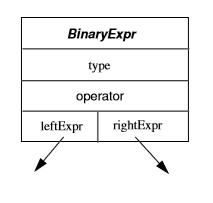
\includegraphics[scale=0.8]{Pictures/AST-B-Exp.png}
  \caption{AST representation of a binary expression}
  \label{fig:ast-binary-expression}
\end{figure}


\newblock
\par
A concrete example is checking the expression $\textit{e}$: $5 + 6$ - we first check the types of operands and learn that both are $\textit{integers}$. Since the operator is a plus, we can type check expression $e$ as $integer$. Type checking is further described in section \cref{sec:design:formal:type-system}.


\section{Compilers and Interpreters}
\label{background:evaluator}

\par
Compilers and interpreters are two types of language implementation systems, and they lie at complete opposite sides of the spectrum. A third type exists, called hybrid, which merges principles of both. This chapter describes the characteristics of each. Based on this, it will argue for our choice. Finally, it will present and explain the implementation details.

The code written in our language is also called the source code. Since it is not written in machine code, the two extremes: the compiler and the interpreter, have different approaches to executing it.

\subsection{Compilers}\label{Evaluator:Compilers}
One way to execute the source code is to translate it into machine code, and this is precisely what the compiler does. Taking the source code as an input, it analyses it: first it splits it up into tokens during the lexing part, and afterwards parses the input to ensure it is properly formed as per the rules of our language. Parsing results in an abstract syntax tree, a simplified representation of the program that still contains all the important information. The semantic analyser walks the tree, verifying that the semantics are correct. Finally, machine code is generated by the code generator. During all the previous phases, the symbol table functions as a database, keeping type and attribute information for user-defined names in the program. The machine code can then be directly run by the computer, which, together with the input of the program, produces the result. The diagram at \cref{fig:compilerdiag} below illustrates this process.

\begin{figure}[!ht]
  \centering
  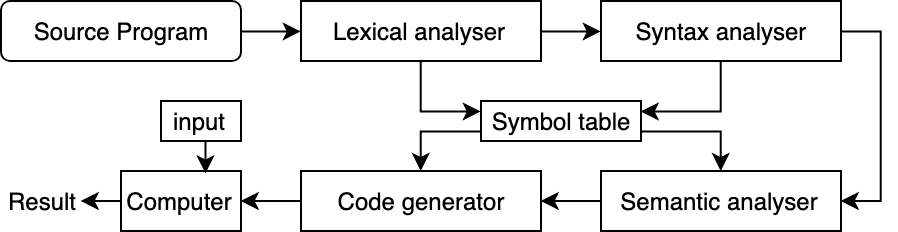
\includegraphics[scale=0.3]{Pictures/compiler-diagram.png}
  \caption{Diagram of a compiler}
  \label{fig:compilerdiag}
\end{figure}

Compiling has the great advantage of performance. After the translation process, which only needs to be performed once, execution is very fast.

\subsection{Interpreters}\label{Evaluator:Interpreters}

As mentioned before, interpreters are polar opposites of compilers as far as language implementation systems go. As opposed to compilers, which translate the source code into machine language in order for it to be executed, interpreters use the interpreter to interpret the source code directly. This can be done without having to translate the code. The interpreter can, therefore, be thought of as a virtual machine for our program.

\par
Interpreters have the advantage of an easier implementation of debugging operations since run-time is tightly knit with the source code. However, it comes at the cost of performance. Execution is 10 to 100 times slower than in compiled systems \cite[p. 50]{concepts-of-programming-languages}, which is the result of decoding the high-level statements. Space is also a disadvantage since the symbol table is needed during execution.

\begin{figure}[!ht]
  \centering
  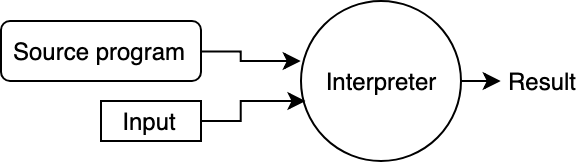
\includegraphics[scale=0.3]{Pictures/interpreter-diagram.png}
  \caption{Diagram of an interpreter}
  \label{fig:interpreterdiag}
\end{figure}

\subsection{Hybrid implementation systems}\label{Evaluator:Hybrid}
Hybrid implementation systems offer a compromise between compilers and interpreters. Hybrid implementation systems share the same front as compilers, but the intermediate code is interpreted as opposed to being translated to machine code. 

\begin{figure}[!ht]
  \centering
  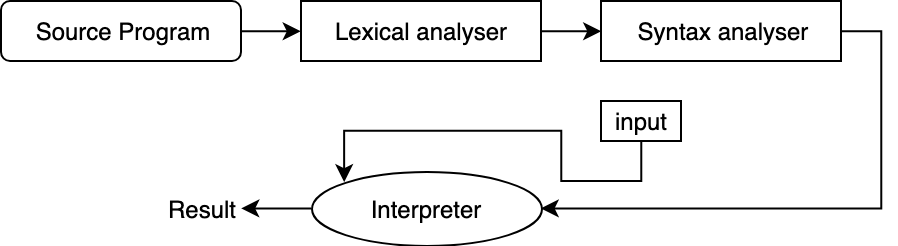
\includegraphics[scale=0.3]{Pictures/hybrid-diagram.png}
  \caption{Diagram of a hybrid implementation system}
  \label{fig:hybriddiag}
\end{figure}


\newpage
\chapter{Language Design}
\label{chap:LanguageDesign} 

AROS is designed to be descriptive and easy to use. Instead of making the programmer focus on the process of an agent and how it should achieve its goal, AROS allows the programmer to just describe what the environment and objectives are. Consequently, AROS computes the optimal process to achieve these objectives, since it is a detail that the programmer does not care about. Rather than writing a program that consists of a set of instructions (e.g. move left, go forward, etc.), the programmer writes a program that describes the environment (size of the area, position and size of obstacles) and the goal. AROS then finds the optimal path for the robot and creates a set of instructions it understands. 

\section{Grid layout}

A grid layout is the foundation of the map layout written in AROS. For a route to be computed, the programmer must have access to all relevant information about the space, which necessarily includes size and obstacles. Most likely, this information will already be presented as a grid. Therefore, recreating it into AROS is simply a matter of setting the dimensions and declaring the obstacles.
\par
A unit's dimension in the AROS grid space is necessarily arbitrary in order to allow different levels of resolution. To program a coffee delivery robot, the resolution of an obstacle might have to be 0.2 meters, for small objects and walls. For a drone or large spaces, however, it might be perfectly fine to keep the resolution at multiple meters per square, both to make programming easier and to reduce the complexity of the computation.
\par
The output of the program will be a series of "up", "down", "left" and "right" commands. These correspond to the robot's movements on the grid. So if the robot is at position (3,3) and receives a "down" command, it will go to the position (4,3). Receiving a "left" command afterwards moves it to (4,2). 
\par
We count on the software running on the robot having these aspects adjustable. Furthermore, an important assumption we make is that the robots are capable of perfectly executing their instructions. Via an array of sensors, if it receives the command "up", it will perform the operation. If it gets stuck or breaks down, it stops the execution. 

\section{Paradigm choice}

Programming languages can be classified based on their features into different paradigms, the main of which are \textit{imperative} and \textit{declarative}.
\par
The imperative programming paradigm allows the programmer to directly describe both the control flow and how the program is executed by changing the state of variables. This allows for constructs such as loops, which are risk-prone due to the fact that different parts of the program can change the same variable.
\par
Declarative programming focuses on the "what" and not the "how". The programmer specifies the properties of the result, not how to compute it. The decision to create a declarative programming language stems from the desire for the language to be a more straightforward and simple approach for declaring a map. Another reason is to differentiate it from the already existing and complex C-like code used for the Arduino platform.
\par
Logic and functional programming are subsets of declarative programming languages.
\par
Logic programming yields the results as the satisfying permutations of states in a defined universe of facts and rules. Using this paradigm would have our language consist of a series of facts describing the obstacles, and then a \textit{path} rule from start to end that would only be satisfied by a valid path.
\par
Functional programming returns the answer as the result of function applications. Due to the property of referential transparency, any function call can be any time replaced by its return value without affecting the result. This is important to our language since we want to always apply transformations going from one version to the map to the next while having the certainty that the previous version is unchanged.
\par
Functional programming also enables us to treat functions as first-class citizens and thus make our language more expressive.
\par
We have therefore decided on using a functional paradigm for AROS. The block structure of the code is familiar to people used to imperative programming, while actually being syntactic sugar for the purely functional "let..in" construct. Immutability enables the programmer to be certain that a defined shape will always stay the same shape, regardless of changes performed on it, without which debugging can possibly be extremely difficult.
\section{Informal overview}

\subsection{Basic types}

\subsubsection{Integer - \lstinline{int}}
    Integers are the basic (and only) numeric type in our language, which serves as the basic building block for higher compositional types.
    \newline \textbf{Examples:} \lstinline{0, 1, 2, 3, 100, 2000, -5, -123}
    
\subsubsection{Boolean - \lstinline{bool}}
    As with many programming languages, Boolean values that can either be true or false and can be used to define decisions and branching in the language.
    \newline \textbf{Examples:} \lstinline{true, false}

\subsubsection{Vector - \lstinline{vec}}
    Vectors in AROS are a composition of two integer components and represent a two-dimensional value, which can be used to define concepts such as size (as values of width and height) or a point on a grid (as coordinates on x and y-axes). 
    \newline \textbf{Examples:} \lstinline{<1,3>, <100,100>, <x,y>}

\subsubsection{List - \lstinline{[]}}
    Lists in AROS are a homogeneous collection of zero to many elements of an arbitrary type. In the context of AROS, they provide a basis for repetition and iteration using higher-order functions. Lists are defined recursively, with two components: a \textit{head} (first element) and a tail (a list containing the rest of the elements).
    \newline \textbf{Examples:}
    \begin{lstlisting}[language=aros,caption=List type examples]
        [int] ints = [1,2,3];
        [vec] vecs = [<1,2>, <3,4>, <5,6>];
    \end{lstlisting}

\subsubsection{Set - \lstinline{\{\}}}
    Similarly to lists, sets are also a collection of homogeneous elements, however, as with mathematical sets, they only allow distinct elements and do not maintain any particular order. Sets are very fundamental in AROS, as they provide the core structure for the definition of grid-based zone layouts. The need for sets as this core structure stems from the nature of defining zone layouts in the form of points on a grid, where non-distinct elements (overlapping points) would bear no meaning.
    \newline \textbf{Examples:} \lstinline|{<1,1>, <1,2>, <1,3>}, {1,2,3}, {true, false}|

\subsubsection{Function - \lstinline{[]}}
    Functions provide an abstraction over expressions, by encapsulating an arbitrary expression inside a local scope. This local scope contains the values of parameters, which are stated when a function is declared and passed into the local scope when the function is called, and the values of local variables declared inside the function body before the return expression. Both the function parameters and the local variables are optional.
    
\newblock
\par 
    In AROS, functions are treated as first-class citizens, and therefore can be used as parameters and/or return expressions of other functions.
    \newline \textbf{Example:}
    \begin{lstlisting}[language=aros,caption=Function type examples]
        (int -> int) addOne = (int) n -> int { n + 1 };
        int two = addOne(1); // two == 2
        
        (-> vec) makeConstVec = () -> vec {
            int x = 10;
            int y = 20;
            <x, y>
        };
        vec myVec = makeConstVec(); // myVec == <10,20>
        
        (int, int -> vec) makeDoublePoint = (int x, int y) -> vec {
           // local declarations 
           int doubled_x = x * 2;
           int doubled_y = y * 2;
           // expression
           <doubled_x, doubled_y>
        }; 
        vec point = makeDoublePoint(2, 2); // point == <4,4>
    \end{lstlisting}

\subsection{Operations}
\subsubsection{Basic arithmetic}
    AROS provides standard binary arithmetic operators for integers: \lstinline{+} for addition, \lstinline{-} for subtraction, \lstinline{*} for multiplication and \lstinline{/} for division. As integers are the only numeric type in AROS, division of two integers is defined as the nearest integer after their division: 
    \begin{equation*}
        \lfloor\frac{a}{b}\rceil
    \end{equation*}
    where $a$, $b$ are integers 
    \newline \textbf{Examples:}
    \begin{lstlisting}[language=aros, caption=Basic arithmetic examples]
        int one = 1;
        int two = one + one;   // two == 2 
        int four = two * two;  // four == 4 
        int four = two * two;  // four == 4 
        int three = 22 / 7;    // three == 3
    \end{lstlisting}
\subsubsection{Comparison operators}
    The comparison operators in AROS are also pretty standard compared to other mainstream programming languages. The equality operator $==$, which can be applied to all types, returns $true$ or $false$ if both operands are structurally equal. Similarly, there is also an inequality operator with symbol $!=$.
    \par The rest of the comparison operators only applied to integers and include:
    \begin{itemize}
        \item Greater than ($>$)
        \item Greater than or equal ($>=$)
        \item Less than ($<$)
        \item Less than or equal ($<=$)
    \end{itemize}
    \textbf{Examples:}
    
    \begin{lstlisting}[language=aros,caption=Comparison operator examples]
        // Integers
        5 == 5                           // true
        5 != 6                           // true
        2 > 1                            // true
        2 >= 1                           // true
        2 >= 2                           // true
        3 < 4                            // true
        3 <= 4                           // true
        3 <= 3                           // true
        
        // Booleans
        true == true                     // true
        true != false                    // true
        
        // Vectors
        <1,3> == <4,5>                   // false
        <1,3> != <4,5>                   // true
        <1,3> == <1,3>                   // true
        
        // Lists
        [1,2,3] == [1,2,3]               // true 
        [3,2,1] == [1,2,3]               // false
        [<1,2>, <3,4>] == [<1,2>, <3,4>] // true
        [<1,2>, <3,4>] == [<3,4>, <1,2>] // false
        
        // Sets
        {1,2,3} == {1,2,3}               // true 
        {3,2,1} == {1,2,3}               // true
        {<1,2>, <3,4>} == {<1,2>, <3,4>} // true
        {<1,2>, <3,4>} == {<3,4>, <1,2>} // true
        
    \end{lstlisting}
\subsubsection{Boolean logic}
    AROS also provides standard binary and unary operators for working with Boolean values, based on predicate logic. These are $and$ (true when both operands true), $or$ (true when either of operands true) and $not$ (negation). The $and$ and $or$ operators are short-circuited, therefore, the evaluation of the second operand may be skipped in case the result can be inferred from just the first operand.  
    \newline \textbf{Examples:}
    \begin{lstlisting}[language=aros,caption=Boolean logic examples]
        5 > 4 and 4 < 5       // true 
        5 > 4 or 5 < 4        // true
        not (5 > 4) and 5 > 4 // false
        not (5 > 4) or 5 > 4  // true
    \end{lstlisting}
\subsubsection{Vector operations}
    The integer arithmetic operators in AROS - $+$, $-$, $*$, $/$ - are overloaded to be also usable on vectors. Applying such operator on two vectors $v1$ and $v2$ will result in a new vector, whose components will be the results of applying the equivalent arithmetic operator pairwise to the respective components of $v1$ and $v2$. 
    \newline Apart from these operations, we can also access the $x$ and $y$ component of a vector by using the $vecx$ and $vecy$ keywords respectively, followed by the vector expression.
    \newline \textbf{Examples:}
    \begin{lstlisting}[language=aros,caption=Vector operation examples]
        vec v1 = <5,3>;
        vec v2 = <2,4>;
        vec added = v1 + v2;       // added == <7,7>
        vec subtracted = v1 - v2;  // subtracted == <3,-1>
        vec multiplied = v1 * v2;  // multiplied == <10,12>
        vec divided = v1 * v2;     // divided == <3,1>
        
        vec vector = <19,20>;
        int x = vecx vector;       // x == 19;
        int y = vecy vector;       // x == 20;
    \end{lstlisting}
\subsubsection{List operations}
    When it comes to (linked) lists in AROS, we can access the $head$ and $tail$ components of a list by using the special keywords `head` and `tail` respectively, followed by an expression of type list. To build a list dynamically, it is possible to use the cons operator ($:$) to prepend a new element onto a list. Additionally, we can also concatenate lists by using the append operator $++$. Given lists $l1$ and $l2$, the concatenation $l1 ++ l2$ evaluates to a new list, which begins with the elements of $l1$, which are followed by the elements of $l2$.
    \newline \textbf{Examples:}
    \begin{lstlisting}[language=aros,caption=List operation examples]
        [int] somePrimes = [13, 17, 19, 23, 29];
        int first = head somePrimes;      // first == 2
        [int] rest = tail somePrimes;       // rest == [3, 5, 7, 11]
        [int] morePrimes =  2 : 3 : 5 : 7 : 11 : []  // demonstrating the cons operator
        [int] myPrimes = morePrimes ++ somePrimes;
        // myPrimes == [2, 3, 5, 7, 11, 13, 17, 19, 23, 29]
    \end{lstlisting}

    
\subsubsection{Set operations}
    As mentioned before, sets are a fundamental feature of AROS and therefore the language natively provides several operators for sets.
    \par The most basic operators are union and intersection with their respective symbols $<>$ and $><$. These follow their mathematical definitions and can be applied to sets with elements of any type.
    \par \textbf{Examples:}
    \begin{lstlisting}[language=aros,caption=Union and intersection examples]
        // Integer sets
        {int} intSet1 = {1,2,3,4,5};
        {int} intSet2 = {4,5,6,7,8};
        {int} intUnion = intSet1 <> intSet2;
        // intUnion == {1,2,3,4,5,6,7,8}
        {int} intInters = intSet1 >< intSet2;
        // intInters == {4,5}
        
        // Vector sets
        {vec} vecSet1 = {<1,2>, <3,4>, <5,6>};
        {vec} vecSet2 = {<3,4>, <5,6>, <7,8>};
        {vec} vecUnion = vecSet1 <> vecSet2;
        // vecUnion == {<1,2>, <3,4>, <5,6>, <7,8>}
        {vec} vecInters = vecSet1 >< vecSet2;
        // vecInters == {<3,4>, <5,6>}
    \end{lstlisting}
    \par Moreover, there are two additional domain specific operators for sets of \textit{vectors}, to facilitate definitions and transformations in the context of points in a grid-based zone layout. Both of these take a set as their first argument, a vector as their second argument, and evaluate to a new set.
    \par The first one is the shift operator with symbol $>>$ which will evaluate to a set of vectors, equivalent to adding the vector argument of $>>$ to each vector in the set argument of $>>$. In the context of the zone, this will \textit{shift} or move the shape defined by the set of vectors.
    \par To give an example, we can show how we can build a shape out of 2 horizontal and 1 vertical lines, using the union and the shift operator: 
    \begin{lstlisting}[language=aros,caption=Examples of the shift operator, label=lst:shift-operator]
        {vec} vertical   = {<0,0>,<1,0>,<2,0>,<3,0>,<4,0>,<5,0>};
        {vec} horizontal = {<0,0>, <0,1>, <0,2>, <0,3>, <0,4>};
        
        // Make new (middle) vertical,
        // by shifting the original 2 coordinates to the right
        {vec} middleVertical = vertical >> (0, 2);
        // middleVertical == {<0,2>,<1,2>,<2,2>,<3,2>,<4,2>,<5,2>}
        
        // Make new (upper) horizontal,
        // by shifting the original 1 coordinate down
        {vec} upperHorizontal = horizontal >> (1, 0);
        // upperHorizontal == {<1,0>, <1,1>, <1,2>, <1,3>, <1,4>};
        
        // Make new (lower) horizontal,
        // by shifting the upper horizontal 3 coordinates down
        {vec} lowerHorizontal = upperHorizontal >> (3, 0);
        // lowerHorizontal == {<4,0>, <4,1>, <4,2>, <4,3>, <4,4>};
        
        // Group the lines into a single shape with union
        {vec} myShape = middleVertical 
                     <> upperHorizontal
                     <> lowerHorizontal;
        // myShape == {
        // <0,2>,<1,0>,<1,1>,<1,2>,<1,3>,<1,4>,<2,2>,
        // <3,2>,<4,0>,<4,1>,<4,2>,<4,3>,<4,4>,<5,2>
        //}
    \end{lstlisting}
    The set of vectors, $myShape$ built in this example, may be seen illustrated in the following figure:
    \begin{figure}[H]
        \centering
        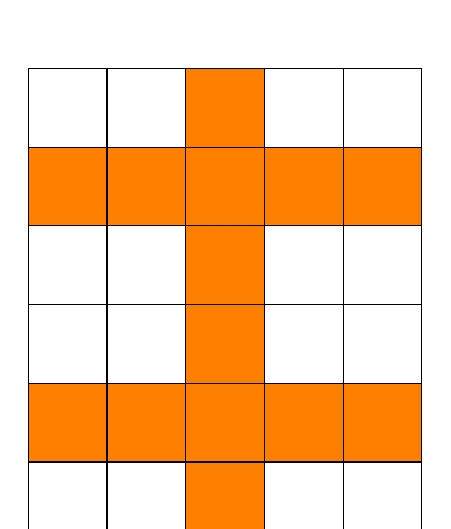
\begin{tikzpicture}[every node/.style={minimum size=1cm-\pgflinewidth, outer sep=0pt}]
            \draw[step=1cm, color=black] (0,0) grid (5,6);
            \node[fill=orange] at (2.5,5.5) {};
            
            \node[fill=orange] at (0.5,4.5) {};
            \node[fill=orange] at (1.5,4.5) {};
            \node[fill=orange] at (2.5,4.5) {};
            \node[fill=orange] at (3.5,4.5) {};
            \node[fill=orange] at (4.5,4.5) {};
            
            \node[fill=orange] at (2.5,3.5) {};
            \node[fill=orange] at (2.5,2.5) {};
            \node[fill=orange] at (2.5,1.5) {};
            \node[fill=orange] at (2.5,0.5) {};
            
            \node[fill=orange] at (0.5,1.5) {};
            \node[fill=orange] at (1.5,1.5) {};
            \node[fill=orange] at (3.5,1.5) {};
            \node[fill=orange] at (4.5,1.5) {};
        \end{tikzpicture}
        \caption{Illustration of shape represented by vector set $myShape$ built in \cref{lst:shift-operator}}
    \end{figure}
    \par The other operator specific to vector-sets is also contextual to defining shapes in the zone, called (and symbolized as) $crop$. The crop operator will remove any vectors from the set (first argument) based on their $x$ and $y$ components, if either of the following is true:
    \begin{itemize}
        \item $v_x > c_x - 1$
        \item $v_y > c_y - 1$
    \end{itemize}
    where $v_x$ , $v_y$ and $c_x$, $c_y$ are $x$ and $y$ components of a vector in the set and the vector argument of the $crop$ operation respectively.
    Effectively, this crops a shape (set of vectors) in a zone into a given width and height, specified in the $x$ and $y$ components of the vector argument of the operation. We can illustrate this on the previously created shape in the following code example:
    
    \begin{lstlisting}[language=aros,caption=Example of using the crop operator, label=lst:cropped-shape]
        {vec} myShapeCropped = myShape crop (5,3);
        // myShapeCropped == {
        // <0,2>,<1,0>,<1,1>,<1,2>,<2,2>,
        // <3,2>,<4,0>,<4,1>,<4,2>
        //}
    \end{lstlisting}
    
Which would result in the following shape:
    
    \begin{figure}[H]
        \centering
        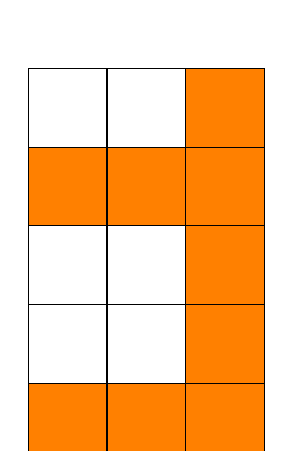
\begin{tikzpicture}[every node/.style={minimum size=1cm-\pgflinewidth, outer sep=0pt}]
            \draw[step=1cm, color=black] (0,0) grid (3,5);
            \node[fill=orange] at (0.5, 0.5) {};
            \node[fill=orange] at (1.5, 0.5) {};
            \node[fill=orange] at (2.5, 0.5) {};
            \node[fill=orange] at (2.5, 1.5) {};
            \node[fill=orange] at (2.5, 2.5) {};
            \node[fill=orange] at (2.5, 3.5) {};
            \node[fill=orange] at (2.5, 4.5) {};
            \node[fill=orange] at (0.5, 3.5) {};
            \node[fill=orange] at (1.5, 3.5) {};
        \end{tikzpicture}
        \caption{Illustration of shape represented by the cropped vector set $myShapeCropped$ built in \cref{lst:cropped-shape}}
    \end{figure}

\subsection{Constructs and Abstractions}
\subsubsection{Functions}
With AROS being a functional language, functions play a fundamental role as abstractions over expressions. Functions can be used to create an expression by constructing it gradually, in several steps (local declaration) in an isolated scope. Functions may be parameterized such that the resulting expression will be constructed and/or evaluated relative to the value(s) provided to the function.

\par{} The main primitive for defining and working with functions is a \textit{lambda} or anonymous function. Lambdas are treated equally to other expressions and act as literals of the function type, in the same way as there are literals for the vector or integer types. Consequently, a function \textit{definition} in AROS, is simply a variable declaration, with a function type and a value in the form of a lambda. An example of this may be seen in the following code listing:
    \begin{lstlisting}[language=aros, float=htb, caption= Function definition by binding a lambda literal to a name]
        (vec, vec -> [vec]) getSquareCoords = (vec bottomLeft, vec topRight) -> [vec] {
            vec topLeft = < (vecx bottomLeft), (vecy topRight) >;
            vec bottomRight = < (vecx topRight), (vecy bottomLeft) >;
            
            [bottomLeft, topLeft, topRight, bottomRight]
        };
    \end{lstlisting}
In the example, a function of type \lstinline{(vec, vec -> [vec])} (two vector parameters + vector list output), named \lstinline{getSquareCoords} has been defined. The function, given two vectors as coordinates of the bottom, left and top right corners of a square returns a list of all the four corners of that square. This example demonstrates how local scope and declarations can be used to define more complicated expression in a much more readable and writable way. 

\par{} Once a function is bound to a name (variable), it is possible to evaluate the function using function application and, for example, bind the evaluated value to a new variable:
    \begin{lstlisting}[language=aros, caption= Function application example]
        [vec] fiveByFive = getSquareCoords(<4,0>, <0,4>);
        // fiveByFive == [<4,0>, <0,0>, <0,4>, <4,4>]
    \end{lstlisting}
\par{} Alternatively, a lambda literal may be evaluated directly, without binding, such as in the following example:
    \begin{lstlisting}[language=aros,float=htb,caption= Direct application of a lambda literal]
        int twoSquared = ((int n) -> int { n * 2 })(2);
        // twoSquared == 4
    \end{lstlisting}

\subsubsection{Conditional expressions}
Decisions based on boolean expressions are facilitated using two main constructs: \lstinline{if} expressions and \lstinline{cond} expressions. As the naming suggests, as the majority of AROS, these are also expressions and therefore may be directly evaluated and bound to variables.

\par As is standard in many programming languages, \lstinline{if} expressions consists of three components: the \textit{condition} and two expressions of same type, call them \lstinline{e1} and \lstinline{e1}. When the entire if expression is evaluated, it will result in either \lstinline{e1} or \lstinline{e2}, based on whether the condition evaluated to \lstinline{true} or \lstinline{false} respectively. An example may be seen in the listing below: 
    \begin{lstlisting}[language=aros, caption= Example of an if expression]
        int x = 10;
        vec a = if (x < 10) { 
            <0,0>    
        } else {
            <10, 10>
        };
        // a == <0,0>
    \end{lstlisting}

\par AROS also makes available another conditional expression, \lstinline{cond}, for situations where the branching consists of more than two branches (and therefore more than one conditions). While this is technically possible to do by nesting \lstinline{if} expressions, \lstinline{cond} provides this functionality in a more concise syntax, giving the users more readability and writability. The following listing contains an example of this construct:

    \begin{lstlisting}[language=aros, caption= Example of a cond expression]
        int x = 100;
        vec a = cond {
            ((x > 0) and (x < 10)) {
                <0,0>
            }
            ((x >= 10)  and (x < 20)) {
                <10,10>
            }
            ((x >= 20) and (x < 30)) {
                <20,20>
            }
            otherwise { <100,100> }
        }; // a == <100, 100>
    \end{lstlisting}
    
\subsubsection{Recursion and Iteration}
In order to execute repetitive computations in a functional style, recursion (function calling itself) can be used. For example, the following code listing includes an implementation of calculating the n-th Fibonacci number recursively:
    \begin{lstlisting}[language=aros, label=lst:fibr, caption= Recursive implementation of calculating n-th Fibonacci number]
        (int -> int) fibr = (int n) -> int {
            cond {
               ((n == 0) or (n == 1)) { n } 
               otherwise { 
                    fibr(n-1) + fibr(n-2)
               }
            }
        }
        int fib5 = fibr(5);
        // fib10 == 55
    \end{lstlisting}

\par{} While \cref{lst:fibr} is sufficient to illustrate recursion, it is a very inefficient implementation. The complexity of this implementation is exponential, due to the repeated recursions stemming from line 5 in \cref{lst:fibr}. The complexity of calculating n-th Fibonacci number can be significantly increased by using an iterative approach. Even though AROS is a functional language and therefore does not support iterative control structures such as a $while$ loop or a $for$ loop, we can make an iterative implementation by passing accumulator values in recursion. The example in 

\newblock

    \begin{lstlisting}[language=aros, label={lst:fibi}, caption= Iterative implementation of calculating n-th Fibonacci number]
        (int, int, int -> int) fibi_h = (int n, int a, int b) -> int {
            cond {
               (n == 0) { a } 
               (n == 1) { b }
               otherwise { 
                    fibi_h(n-1, b, a + b)
               }
            }
        };
        
        (int -> int) fibi = (int n) -> int {
            fibi_h(n, 0, 1)
        };
        
        int fib5 = fibi(5);
        // fib10 == 55
    \end{lstlisting}

\subsubsection{Generic higher-order functions}

\par 
In a functional language paradigm, higher-order function, such as map, filter and fold, are commonly used to solve particular problems. They are in fact, so frequent and versatile, that we have decided to incorporate them into the syntax of AROS. 

\par 
Map takes a function $f$ and a list $l_1$ and applies that function $f$ to every element in the list $l_1$, producing a new list $l_2$. The type scheme of a map is $((\alpha \rightarrow \beta), [\alpha] \rightarrow [\beta])$, meaning that the argument of function $f$ must have the same type as element of list $l_1$ and the return type of function $f$ must be the same as the type of the element of $l_2$. The following example utilizes map to shift every x coordinate of a vector in a list by 1.

\newblock 
\begin{lstlisting}
    (vec -> vec) f = (vec v) -> vec {
        int x = vecx v;
        int y = vecy v;
        <x + 1, y>
    };
    
    [vec] l = [<1,1>, <1,2>, <1,3>];
    
    [vec] new_l = map(f, l); 
    //new_l == [<2,1>, <2,2>, <2,3>]
\end{lstlisting}

\newblock
\par 
Filter takes a predicate (a function $f$, which returns a boolean value) and a list $l_1$ and returns a list $l_2$, consisting of elements of $l_1$ that satisfy the predicate. The type scheme of a filter is $((\alpha \rightarrow Bool), [\alpha] \rightarrow [\alpha])$, meaning that the type of argument of $f$ and the type of elements of both lists $l_1$ and $l_2$ must be equal. The following example utilizes filter to filter out empty sets from a list.

\newblock 
\begin{lstlisting}
    ({vec} -> bool) f = ({vec} s) -> bool {
        s != {}
    };
    
    [{vec}] l = [{<1,1>, <1,2>, <1,3>}, {}, {<0,0>}, {}];
    
    [vec] new_l = filter(f, l); 
    //new_l == [{<1,1>, <1,2>, <1,3>}, {<0,0>}]
\end{lstlisting}

\newblock
\par
A fold (right) takes a function, a starting value (an accumulator) and a list to fold up. The function itself takes two parameters. The function is called with the accumulator and the last element and produces a new accumulator. Then, the function is called again with the new accumulator and the now new last element, and so on. Once we have walked over the whole list, only the accumulator remains, which is what we have reduced the list to. \cite[p. 61]{learn-you-a-haskell-for-great-good} The type scheme of fold right is $((\alpha, \beta \rightarrow \beta), \beta, [\alpha] \rightarrow \beta)$. The following example is an implementation of the above map, using the right fold.

\begin{lstlisting}
    ((vec -> vec), [vec] -> [vec]) map' = ((vec -> vec) f, [vec] l) -> [vec]{
        (vec, [vec] -> [vec]) f' = (vec h, [vec] a) -> [vec] {
            f(h) : a
        }
        foldr(f', [], l)
    }
\end{lstlisting}

\subsubsection{Domain specific constructs}
As mentioned in the previous sections, the key objective of every program written in AROS is to define the map, obstacles and route from the robot's current position to its goal. Therefore, there are two specific constructs that have to be present at the end of every program written in AROS - the grid and route definitions. 

 \par
 The grid definition begins with a $\textit{grid}$ keyword followed by two expressions separated by a comma. The first expression represents the size of the grid and therefore must evaluate to a vector. The second expression must evaluate to a set of vectors because it represents all the obstacles on the grid. Any obstacles defined beyond the size of the grid will simply be discarded. 
 
 \par 
 The route definition begins with a $\textit{route}$ keyword, which is similarly followed by two expressions, separated by a comma. The expressions define the starting and ending position of the path that a robot has to undertake. Both of these expressions have to evaluate to a vector. The following demonstrates the usage of these constructs.
 
 \newblock
 
\begin{lstlisting}
    vec size = <5,5>;
    {vec} obstacles = {<1,1>,<2,2>,<3,3>};
    vec start = <0,0>;
    vec end = <4,4>
    
    grid size, obstacles
    route start, end
\end{lstlisting}
\section{Formal specification}\label{section:Specification}

\subsection{Abstract grammar}
\label{sec:abstract-grammar}

\par
In this section, we give a formal description of the AROS language, such that it is clear which programs are syntactically valid and which are not. We first define it by means of the abstract grammar. 

\par
Abstract grammar is a context-free grammar, which provides a clearer, simplified syntactic description of the language. However, compared to a concrete grammar, it may be ambiguous and it is not concerned with e.g. operator precedence, etc. The abstract syntax is defined by a collection of syntactic categories and a finite set of formation rules for every syntactic category.

\par
The abstract grammar of AROS consists of the following syntactic categories:


\begin{align*}
    & i \in \mathbf {Int} - \text{Integers} \\
    & b \in \mathbf {Bool} - \text{Booleans} \\
    & x \in \mathbf {Var} - \text{Variables} \\ 
    & e \in \mathbf {Exp} - \text{Expression} \\
    & T \in \mathbf {Type} - \text{Types} \\
    & P \in \mathbf {Params} - \text{Function parameters} \\
    & L \in \mathbf {Lambda} - \text{Lambda expression} \\
    & B \in \mathbf {Block} \\
    & FA \in \mathbf {FunctionApplication} \\
    & D \in \mathbf {Dec} - \text{Declaration} \\
    & G \in \mathbf {GridDef} - \text{Grid definition} \\
    & R \in \mathbf {RouteDef} - \text{Route definition} \\
    & Prog \in \mathbf {Program}
    &&&
\end{align*}

\newblock
\par
An arbitrary element of a syntactic category is represented by meta-variables. For example, $e$ is a meta-variable for expression, L is a meta-variable for lambda, etc. Members of the above mentioned syntactic categories are defined by sets of formation rules:

\begin{flalign*}
    & T ::= int\\
        &\quad \quad \: | \: bool \\
        &\quad \quad \: | \: vec \\
        &\quad \quad \: | \: [T] \\
        &\quad \quad \: | \: \{T\} \\
        &\quad \quad \: | \: ( [T,]^* T \rightarrow T ) \\
        &\quad \quad \: | \: ( \rightarrow T ) \\ \\
    & e ::= x \\
        & \quad \quad | \: i \\
        & \quad \quad | \: b \\
        & \quad \quad | \: <e,e> \\
        & \quad \quad | \: [ [e,]^* e]\\
        & \quad \quad | \: [ \: ] \\
        & \quad \quad | \: \{ [e,]^* e \} \\
        & \quad \quad | \: \{ \: \} \\
        & \quad \quad | \: (e) \\
        & \quad \quad | \: o_1 \: e \\
        & \quad \quad | \: e \: o_2 \: e \\
        & \quad \quad | \: L \\
        & \quad \quad | \: FA \\
        & \quad \quad | \: if(e) \: B \: else \: B\\
        & \quad \quad | \: cond\{\: [(e) \: B]^+ \: otherwise \: B \} \\
        & \text{where } \\
        & \quad o_1 \in \{ not, \: head, \: tail, \: vecx, \: vecy\} \\
        & \quad o_2 \in \{ +, \: -, \: *, \: / , \: ++, \: : , \: <> , \: >< , \: >> , \: crop , \: and, \: or , \: > , \: < , \: >= , \: <= , \: == , \: != \} \\ \\
    & FA ::= x \: P \\
         & \: \: \: \: \quad \quad | \: L \: P \\
         & \: \: \: \: \quad \quad | \: map (e, e) \\
         & \: \: \: \: \quad \quad | \: filter (e, e) \\
         & \: \: \: \: \quad \quad | \: fold (e, e, e)
    &&&
\end{flalign*}

\begin{flalign*}
    & P ::= ([e,]^* \: e) \: | \: ( \lambda ) \\
    & B ::= \{ \: D \: e \} \\ \\
    & L ::= ([T \: x,]^* \: T \: x) \rightarrow T \: B \\
        & \quad \quad | \: \: (\lambda) \rightarrow T \: B \\ \\
    & D ::= T \: x = e; \: D \: | \: \lambda \\
    & G ::= grid \: e, \: e \\
    & R ::= route \: e, \: e \\
    & Prog ::= D \: G \: R\\
    &&&
\end{flalign*}

\par 
The function type $([T,]^* \: T) \rightarrow T$, is just syntactic sugar, allowing multiple input parameters. However, every function type can be redefined by its equivalent curried form. Therefore the type $(T_1, T_2, T_3 \rightarrow \: T_4)$, can be defined as $(T_1 \rightarrow \: (T_2 \rightarrow \: (T_3 \rightarrow \: T_4)))$. This can be illustrated on the following two functions $f$ and $f'$.

\newblock
\begin{lstlisting}[language=aros]
    (int, int, int -> int) f = 
        (int x, int y, int z) -> int {
            x * y * z
    }
    
    (int -> (int -> (int -> int))) f' =
        (int x) -> int {
           (int y) -> int {
                (int z) -> int {
                    x * y * z
                }
            }
        }
\end{lstlisting}

\newblock
\par
We assume that elements of $\textbf{Int}$ are integers, elements of $\textbf{Bool}$ are either $true$ or $false$ and an element of $\textbf{Var}$ is any string containing only letters of Latin alphabet, Arabic numerals and symbol $\_$, starting with a lowercase letter. We can define these categories by means of regular expressions:


\begin{align*}
    & b :== true \: | \: false \\
    & i :== [-]?[1-9][0-9]^* \: | \: 0 \\
    & x :== [a-z][a-zA-Z0-9\_]^* \\
    &&&
\end{align*}

\subsection{Type system}
\label{sec:design:formal:type-system}
\par
As informally described in section XY, values of expressions in the language can be of type integer, boolean, vector, set, list or a function. Types are defined formally using the formation rules in table XYY. Such recursive definition of lists and sets allows nesting, so that a ``list of sets of integers'', $[ \{int\} ]$, is a valid type. 

\par 
Similarly, the same principle applies to functions. They can accept other functions as parameters as well as return functions. While a function is only allowed to return one expression of a given type, it can accept an arbitrary number of input parameters, or no parameters at all. The following are examples of function types allowed in AROS:


\begin{align*}
    & (int \rightarrow bool)\\
    & (int, int \rightarrow vec)\\
    & ((int \rightarrow bool), [int] \rightarrow [bool])\\
    & ( \rightarrow (\{vec\} \rightarrow [vec]))\\
    &&&
\end{align*}

\par
Therefore, the set of valid types in AROS $\textbf{Type}$, is infinite: 

\begin{align*}
    Type = \{ int, bool, vec, [int], [bool], [vec], [[int]], \cdots, (int \rightarrow int), \cdots, (int,(int \rightarrow bool) \rightarrow bool), \cdots \}
\end{align*}

\newblock
\par
Furthermore, we can define two subsets of $\textbf{Type}$:

\begin{align*}
    & \mathbf{SType} \subset \mathbf{Type} - \text{Standard type} \\
    & \mathbf{FType} \subset \mathbf{Type} - \text{Function types} \\  
    & where \: \mathbf{FType} \cap \mathbf{SType} = \emptyset \\
    &&&
\end{align*}

Formation rules for each subset can be defined as follows:

\begin{align*}
    & T_s ::= int \: | \: bool \: | \: vec \: | \: [T] \: | \: \{T\} \text{,where } T_s \in \mathbf{SType} \\
    & T_f ::= ([T,]^*T \rightarrow T) \: | \: (\rightarrow T) \text{,where } T_f \in \mathbf {FType} \\
    &&&
\end{align*}

\newblock
\par
According to the abstract grammar, it is syntactically correct to write an expression such as $10+\{true, false\} $. Such expression, of course, does not make sense and it is hard to imagine how a number 10 can be added to a set of Boolean values. The goal of a type system is to ensure type safety by disallowing such expressions.

\par
Declarations of variables is an essential language construct in AROS. It is necessary to keep track of types of these variables so that we will be able to correctly evaluate expressions containing them. To do this, we use \textit{E} as the type environment. The type environment $E$ can be defined as a partial function: 

\begin{align*}
    E: Var \rightharpoonup Type
\end{align*}

where
\begin{itemize}
    \item $Var$ is a set of declared variables
    \item $Type$ is a set of types
    \newline
\end{itemize}

\par
To update a type environment with a new declaration of variable $x$ of type $T$ we write $E[x \longmapsto T]$, obtaining an updated environment $E'$ defined by: 

\begin{align*}
    E'(y) = \begin{cases} E(y) &\mbox{if } y \neq x \\ 
   T &\mbox{if } y = x \end{cases}
\end{align*}

We can now define type rules that describes how types are assigned to syntactic entities. We employ type judgements of the form:     

\begin{align*}
    E \vdash e : T
\end{align*}

where:
\begin{itemize}
    \item $E$ is a type environment - mapping from declared variables to their types
    \item $e$ is an expression
    \item $T$ is a type
\end{itemize}

\par
In other words, the above definition states that the expression $e$ has type $T$ relative to the type environment $E$.\newline

\par
Type judgements are combined into type rules of the following form:

\begin{align*}
    {\dfrac{J_1; J_2;...;J_n}{J}}
\end{align*}

where:
\begin{itemize}
    \item $J_i$ for $1 \leq i \leq n$ is a premise of the type rule
    \item $J$ is a conclusion of the type rule
\end{itemize}

\par
So that if all the type judgements $J_i$ hold, the conclusion J also holds. We can now describe our type system as follows: 
\begin{flalign}
    & [VAR_{EXP}]\quad {\dfrac{E(x) = T}{E \vdash x \colon T}} &
\end{flalign}

\begin{flalign}
    & [PAR_{EXP}]\quad {\dfrac{E \vdash x \colon T}{E \vdash(x) \colon T}} &
\end{flalign}

\begin{flalign}
    & [INT_{EXP}]\quad {E \vdash i \colon int} &
\end{flalign}

\begin{flalign}
    & [INT\_OP_{EXP}]\quad {\dfrac{E \vdash e_1 \colon int; E \vdash e_2 \colon int}{E \vdash e_1 \:  o \:  e_2 \colon int}}\text{, where } o \in \{+,-,*,/\} &
\end{flalign}

\begin{flalign}
    & [BOOL_{EXP}]\quad {E \vdash b \colon bool} &
\end{flalign}

\begin{flalign}
    & [BOOL\_OP_{EXP}]\quad {\dfrac{E \vdash e_1 \colon bool;E \vdash e_2 \colon bool}{E \vdash e_1 \: o \: e_2 \colon bool}}\text{, where } o \in \{and, or\} &
\end{flalign}

\begin{flalign}
    & [BOOL\_COMP_{EXP}]\quad {\dfrac{E \vdash e_1 \colon int;E \vdash e_2 \colon int}{E \vdash e_1 \: o \: e_2 \colon bool}}\text{, where } o \in \{>,<,>=,<=,==,!=\} &
\end{flalign}

\begin{flalign}
    & [BOOL\_NEGATION_{EXP}]\quad {\dfrac{E \vdash e \colon bool}{E \vdash not \: e \colon bool}} &
\end{flalign}

\begin{flalign}
    & [VEC_{EXP}]\quad {\dfrac{E \vdash e_1 \colon int;E \vdash e_2 \colon int}{E \vdash \langle e_1,e_2 \rangle  \colon vec }} &
\end{flalign}

\begin{flalign}
    & [VEC\_UOP_{EXP}]\quad {\dfrac{E \vdash e \colon vec}{E \vdash o \: e \colon int}}\text{, where }o \in \{vecx, vecy \} &
\end{flalign}

\begin{flalign}
    & [VEC\_BOP_{EXP}]\quad {\dfrac{E \vdash e_1 \colon vec; E \vdash e_2 \colon vec}{E \vdash e_1 \: o \: e_2 \colon vec}}\text{, where }o \in \{+,-,*,/ \} &
\end{flalign}

\begin{flalign}
    & [VEC\_SCAL_{EXP}]\quad {\dfrac{E \vdash e_1 \colon int;E \vdash e_2 \colon vec}{E \vdash e_1 \: * \: e_2 \colon vec}} &
\end{flalign}
\label{page:empty-set-list}
\begin{flalign}
    & [EMPTY\_LIST_{EXP}]\quad E \vdash [\text{ }] : [T] &
\end{flalign}

\begin{flalign}
    & [LIST\_CONS_{EXP}]\quad {\dfrac{E \vdash e_1 \colon T; E \vdash e_2 \colon [T]}{E \vdash e_1 \: \colon \: e_2 \colon [T]}} &
\end{flalign}

\begin{flalign}
    & [LIST\_APPEND_{EXP}]\quad {\dfrac{E \vdash e_1 \colon [T];E \vdash e_2 \colon [T]}{E \vdash e_1  ++  e_2 \colon [T]}} &
\end{flalign}

\begin{flalign}
    & [LIST\_HEAD_{EXP}]\quad {\dfrac{E \vdash e \colon [T]}{E \vdash head \text{ } e \colon T}} &
\end{flalign}

\begin{flalign}
    & [LIST\_TAIL_{EXP}]\quad {\dfrac{E \vdash e \colon [T]}{E \vdash tail \text{ } e \colon [T]}} &
\end{flalign}

\begin{flalign}
    & [SET_{EXP}]\quad {\dfrac{E \vdash e \colon T}{E \vdash \{e\} \colon \{T\}}} &
\end{flalign}

\begin{flalign}
    & [EMPTY\_SET_{EXP}]\quad {E \vdash \{ \text{ }\} \colon \{T\}} &
\end{flalign}

\begin{flalign}
    & [SET\_OP_{EXP}]\quad {\dfrac{E \vdash e_1 \colon \{T\}; E \vdash e_2 \colon \{T\}}{E \vdash e_1 \: o \: e_2 \colon \{T\}}}\text{, where }o \in \{\cup, \cap\} &
\end{flalign}

\begin{flalign}
    & [VECTOR\_SET\_OP_{EXP}]\quad {\dfrac{E \vdash e_1 \colon \{vec\}; E \vdash e_2 \colon vec}{E \vdash e_1 \: o \: e_2 \colon \{vec\}}}\text{, where }o \in \{\gg, *,crop\} &
\end{flalign}

\begin{flalign}
    & [LAMBDA^1_{EXP}]\quad {
    \dfrac
    {E[x_1 \longmapsto T_1, \cdots, x_n \longmapsto T_n] \vdash B \colon T_r}
    {E \vdash (T_1 \: x_1, \cdots,\: T_n \: x_n) \rightarrow \: T_r \: B \colon ( T_1, \cdots, T_n \rightarrow T_r ) }} &
\end{flalign}

\begin{flalign}
    & [LAMBDA^2_{EXP}]\quad {
    \dfrac
    {E \vdash B \colon T}
    {E \vdash ( \lambda) \rightarrow T \: B \colon T }} &
\end{flalign}

\begin{flalign}
    & [IF_{EXP}]\quad {\dfrac{E \vdash e \colon bool; E \vdash B_1 \colon T; E \vdash B_2 \colon T}{E \vdash if(e) B_1  \text{ else } B_2 \colon T}} &
\end{flalign}

\begin{flalign}
    & [COND_{EXP}]\quad {\dfrac{E \vdash e_1 \colon bool; \cdots ; E \vdash e_n \colon bool ; E \vdash B_1 \colon T; \cdots ; E \vdash B_n \colon T, E \vdash B_o \colon T}{E \vdash cond\{ (e_1) B_1 \cdots (e_n) B_n \text{ otherwise } B_o\} \colon T}} &
\end{flalign}

\begin{flalign}
    & [APP\_VAR_{EXP}]\quad {\dfrac
        {E \vdash x \colon (T_1, \cdots,T_n \rightarrow T_r); E \vdash P \colon T_1, \cdots, T_n}
        {E \vdash x \: P \colon T_r}
    } &
\end{flalign}

\begin{flalign}
    & [APP\_LAMBDA_{EXP}]\quad {\dfrac
        {E \vdash L \colon (T_1, \cdots,T_n \rightarrow T_r); E \vdash P \colon T_1, \cdots, T_n}
        {E \vdash L \: P \colon T_r}
    } &
\end{flalign}

\begin{flalign}
    & [APP\_EMPTY_{EXP}]\quad {\dfrac
        {E \vdash L \colon (\rightarrow T)}
        {E \vdash L \: (\lambda) \colon T}
    } &
\end{flalign}

\begin{flalign}
    & [APP\_MAP_{EXP}]\quad {\dfrac
        {E \vdash e_1 \colon (T_1 \rightarrow T_2); E \vdash e_2 \colon [T_1]}
        {E \vdash map(e_1, \: e_2) \colon [T_2]}
    } &
\end{flalign}

\begin{flalign}
    & [APP\_FILTER_{EXP}]\quad {\dfrac
        {E \vdash e_1 \colon (T \rightarrow Bool); E \vdash e_2 \colon [T]}
        {E \vdash filter(e_1, \: e_2) \colon [T]}
    } &
\end{flalign}

\begin{flalign}
    & [APP\_FOLD_{EXP}]\quad {\dfrac
        {E \vdash e_1 \colon (T_1, \: T_2 \rightarrow T_1); E \vdash e_2 \colon T_1; E \vdash e_3 \colon [T_2]}
        {E \vdash fold(e_1, \: e_2, \: e_3) \colon T_1}
    } &
\end{flalign}

\begin{flalign}
    & [PARAMS]\quad {\dfrac
        {E \vdash e_1 \colon T_1; \cdots; E\vdash e_n \colon T_n}
        {E \vdash (e_1,\cdots,e_n) \colon T_1,\cdots,T_n}
    }
    &
\end{flalign}

\begin{flalign}
    & [BLOCK]\quad {\dfrac
        {E \vdash D \: e \colon T}
        {E \vdash \{ D \: e \} \colon T}
    } &
\end{flalign}

\begin{flalign}
    & [EMPTY_{DEC}]\quad {
        \dfrac
        {E \vdash G \colon ok; E \vdash R \colon ok}
        {E \vdash \lambda \: G \: R \colon ok}
    } &&&
\end{flalign}

\begin{flalign}
    & [VAR_{DEC}]\quad { 
        \dfrac
        {E[x \longmapsto T] \vdash D \: G \: R \colon ok; E \vdash e \colon T}
        {E \vdash T \: x =e; \: D \: G \:R \colon ok}
        \text{,where } T \in \mathbf{SType}
    } &&&
\end{flalign}

\begin{flalign}
    & [VAR\_REC_{DEC}]\quad 
    {
        \dfrac
        {E[x \longmapsto T] \vdash D \: G \: R \colon ok; E[x \longmapsto T] \vdash e \colon T}
        {E \vdash T \: x =e; \: D \:G \:R \colon ok}
        \text{,where } T \in \mathbf{FType}
    }&&&
\end{flalign}

\begin{flalign}
    & [EMPTY\_BLOCK_{DEC}]\quad {
        \dfrac
        {E \vdash e \colon T}
        {E \vdash \lambda \: e \colon T}
    }&&&
\end{flalign}

\begin{flalign}
    & [VAR\_BLOCK_{DEC}]\quad {
        \dfrac
        {E[x \longmapsto T] \vdash D \: e' \colon T';E\vdash e \colon T}
        {E \vdash T \: x = e; D \: e' \colon T'}
        \text{,where } T \in \mathbf{SType}
    }&&&
\end{flalign}

\begin{flalign}
    & [VAR\_BLOCK\_REC_{DEC}]\quad
    {
        \dfrac
        {E[x \longmapsto T] \vdash D \: e' \colon T';E[x \longmapsto T]\vdash e \colon T}
        {E \vdash T \: x = e; D \: e' \colon T'}
        \text{,where } T \in \mathbf{FType}
    }&&&
\end{flalign}

\begin{flalign}
    & [GRID]\quad {\dfrac
        {E \vdash e_1 \colon vec; E \vdash e_2 \colon \{vec\}}
        {E \vdash grid \: e_1, \: e_2 \colon ok}
    } &
\end{flalign}

\begin{flalign}
    & [Route]\quad {\dfrac
        {E \vdash e_1 \colon vec; E \vdash e_2 \colon vec}
        {E \vdash route \: e_1, \: e_2 \colon ok}
    } &
\end{flalign}

\newblock
\par
After defining our type system, we can easily observe that the previously mentioned expression: $10 + \{true, false\}$, is a bad expression that is not typable because there is no type rule defining how to add an integer to a set of Booleans.

\par
Some type rules are applicable to any types. For example, the type rule 2.23 states, that a $if expression$ can be of any type, as long as its condition $b$ has type Boolean and both blocks are of the same type. 

\par
We can now employ these type rules and claim that the function on SNIPPET-XY has type $(vec, int \rightarrow [vec])$ and its declaration is $ok$. 

\newblock
\begin{lstlisting}[language=aros]
(vec, int -> [vec]) hr = 
    (vec s, int l) -> [vec] {
        if(l == 0){
            []
        }
        else{
            int l'= l-1;
            int x = vecx s;
            int y = vecy s + l';
            <x, y> : hr(s, l')
        }
}
\end{lstlisting}

\newblock
\par
However, for simplicity reasons, the sample program contains neither a grid nor a route definition and only consists of a single declaration. To validate it, we have to alter global declaration rules, such that, they do not require a grid and route after declarations:

\begin{flalign}
    & [VAR\_TEMP\_REC_{DEC}]\quad 
    {
        \dfrac
        {E[x \longmapsto T] \vdash \text{D} \colon ok; E[x \longmapsto T] \vdash e \colon T}
        {E \vdash T \: x =e; \: D \colon ok}
        \text{,where } T \in \mathbf{FType}
    }&&&
\end{flalign}

\begin{flalign}
    & [EMPTY\_TEMP_{DEC}]\quad {E \vdash \lambda \colon \text{ok}} &&&
\end{flalign}

\begin{align*}
        \dfrac
        {
            \dfrac
            {
            }
            {E[hr \longmapsto (vec, int \rightarrow [vec])] = E^1 \vdash \lambda \colon ok;}
            \quad
            \dfrac
            {
                \dfrac
                {...}
                {E^1[s \longmapsto vec, l \longmapsto int] = E^2 \vdash Block_1 \colon [vec]}
            }
            {E^1 \vdash (vec \: s,\: int \:l) \rightarrow [vec] \:  Block_1 \colon (vec, int \rightarrow [vec])}
        }
        {
            E \vdash (vec, int \rightarrow [vec]) hr = (vec \: s,int \: l) \rightarrow [vec] \: Block_1 \colon ok 
        }
\end{align*}

where $Block_1$ is a substitution for the body of the function $hr$.

\newblock
\par
In order to employ the appropriate type rule, we have to examine the nature of this declaration. It is easy to observe that $hr$ is a function. However, it is also a recursive function, because it is applied directly in its body. To deal with this, we have to use a type rule restricted to the functional declaration - $[VAR\_TEMP\_REC_{DEC}]$. The difference between $[VAR\_REC_{DEC}]$ (or the altered $[VAR\_TEMP\_REC_{DEC}]$) and $[VAR_{DEC}]$ is that the former updates the type environment for both premises. Therefore, when the derivation tree reaches the function application, the variable $hr$ can be looked up in the type environment. Such recursive declarations have been restricted to functional types, since declarations such as $int \text{ } x = 5 * x$ do not make sense in a context of declarative programming language, without assignments or mutations. 

\par
$E^1$ is the updated environment $E$ with variable $hr$ of type $(vec,int \rightarrow [vec])$. Since there are no other declarations, we can apply the $[EMPTY\_TEMP_{DEC}]$ rule, reaching an axiom stating that an empty declaration is $ok$. Furthermore, we have to verify that the expression on the right-hand side of the declaration does have the stated type. Employing the $[LAMBDA^1_{EXP}]$ rule, we first update the environment $E^1$ with function parameters and their types. It is important to note, that if there were other declarations in the sample program, this update would not leak to other branches of the derivations tree, preserving the scope of the function. Next, we have to verify that the function body evaluates to the expected return type. To progress the right branch of the derivation tree, we substitute back the function body for $Block_1$.



\begin{align*}
    \dfrac
    {
        \dfrac
        { \dfrac
        {
            \dfrac{\dfrac{}{E^2(l) = int}}{E^2 \vdash l \colon int;}
            \dfrac{}{E^2 \vdash 0 \colon int}
        }
        {E^2 \vdash l == 0 \colon bool;}
        \quad
        \dfrac
        {\:}
        {E^2 \vdash [ \: ] \colon [vec];} 
        \quad
        \dfrac
        {...}
        {E^2 \vdash Block_2 \colon [vec]}}
        {E^2 \vdash if (l == 0) \{ [ \: ] \} \: else \: Block_2 \colon [vec]}
    }
    {
        E^2 \vdash \{ \: if (l == 0) \{ [ \: ] \} \: else \: Block_2 \: \} \colon [vec]
    }
\end{align*}

where $Block_2$ is a substitution for the body of the else block.

\par
To continue the derivation we first use the $[BLOCK]$ rule to remove the outer curly brackets. Then, by application of the $[IF_{EXP}]$ type rule, we check that the condition is of type Bool and that both blocks return type $[vec]$. To validate the type of the Boolean expression, we employ the $[BOOL\_COMP_{EXP}]$ rule and check that both variable $l$ and $0$ are integers. The variable $l$ can be looked up in the type environment $E^2$ since:

\begin{flalign}
    E^2 = hr:(vec,int \rightarrow [vec]), s:vec, l:int   
\end{flalign}

\newblock
\par
The first block of the $if expression$ is an axiom $[EMPTY\_LIST_{EXP}]$. We can now substitute back $Block_2$ and continue the derivation.

\begin{align*}
    \dfrac
    {
        \dfrac
        {
        \dfrac
            {\dfrac{\dfrac{}{E^2(l) = int}}{E^2 \vdash l \colon int;}
             \dfrac{}{E^2 \vdash 1 \colon int}
            }
            {E^2 \vdash l - 1 \colon int;}
        \dfrac
            {
                \dfrac
                {
                    \dfrac
                    {
                        \dfrac
                        {}
                        {E^3(s) = vec}
                    }
                    {E^3 \vdash s \colon vec}
                }
                {E^3 \vdash vecx \: s \colon int; }
                \quad
                \dfrac
                {...}
                {E^3[x \longmapsto int] = E^4 \vdash Decs_1 \: Exp_1 \colon [vec]}
            }
            {E^2[l' \longmapsto int] = E^3 \vdash int \text{ } x = vecx  \text{ }  s; Decs_1 \: Exp_1 \colon [vec]}
        }
        {E^2 \vdash int \: l' = l - 1; int \text{ } x = vecx \: s; Decs_1 Exp_1 \colon [vec]}
    }
    {E^2 \vdash \{ \: int \text{ } l' = l - 1; int \text{ } x = vecx \text{ } s; Decs_1 Exp_1 \} \: \colon [vec]}
\end{align*}

where $Decs_1$ is a substitution for the reminding declarations and $Exp_1$ is an expression in the else block. 

\newblock
\par
To confirm that the else block does evaluate to type $[vec]$, we again start by applying the $[BLOCK]$ rule. Then we have to recursively apply rule $[VAR\_BLOCK_{DEC}]$ and validate that each local declaration holds. Local declarations also update the type environment. The expression $l - 1$ is verified using the $[INT\_OP_{EXP}]$ rule and expression $vecx \text{ } s$ is verified using the $[VEC\_UOP_{EXP}]$ rule. We can now substitute back the remaining declarations and the expression.

\begin{align*}
    \dfrac
    {
        \dfrac
        {
            \dfrac
            {
                \dfrac
                {\dfrac{}{E^4(s) = vec}}
                {E^4 \vdash s \colon vec}
            }
            {E^4 \vdash vecy \text{ } s \colon int;} 
            \dfrac
            {\dfrac{}{E^4(l') = int}}
            {E^4 \vdash l' \colon int}}
        {E^4 \vdash vecy \: s + l' \colon int}
        \dfrac
        {
            \dfrac
            {
                \dfrac
                {
                    \dfrac
                    {\dfrac{}{E^5(x) = int}}
                    {E^5 \vdash x \colon int}
                    \dfrac
                    {\dfrac{}{E^5(y) = int}}
                    {E^5\vdash y \colon int}
                }
                {E^5 \vdash (x,y) \colon vec}
                \dfrac
                {...}
                {E^5 \vdash hr(s,l') \colon [vec]}
            }
            {E^5 \vdash (x,y) \colon hr (s, l') \colon [vec]}
        }
        {E^4[y \longmapsto int] = E^5 \vdash \lambda (x,y) \colon hr (s, l') \colon [vec]}
    }
    {E^4 \vdash int \: y = vecy \: s + l'; (x, y) \colon hr(s, l') \colon [vec]}
\end{align*}

\newblock
\par
We continue with the recursive application of the $[VAR\_BLOCK_{DEC}]$ type rule. Similarly to previous declarations, the expression on the right hand side, $vecy \text{ } s + l'$, is validated by rules $[INT\_OP_{EXP}]$ and $[VEC\_UOP_{EXP}]$. After concluding that the last local declaration in the else block is type safe, we use the $[EMPTY\_BLOCK_{DEC}]$ rule. Now we just have to verify the remaining block expression. The expression is a cons operation and so the $[LIST\_CONS_{EXP}]$ rule is used. The following derivation verifies that the expression $hr(s,l')$ has type $[vec]$.

\begin{align*}
    \dfrac
    {
        \dfrac
        {\dfrac{}{E^5(hr) = (vec,int \rightarrow [vec])}}
        {E^5 \vdash hr \colon (vec,int \rightarrow [vec])}
        \quad
        \dfrac
        {
            \dfrac
            {\dfrac{}{E^5(s) = vec}}
            {E^5 \vdash s \colon vec}
            \dfrac
            {\dfrac{}{E^5(l') = int}}
            {E^5 \vdash l' \colon int}
        }
        {E^5 \vdash (s,l') \colon vec,int}
    }
    {E^5 \vdash hr(s,l') \colon [vec]}
\end{align*}

\newblock
\par
The expression $hr(s,l')$ is a function application and so we use the $[APP\_VAR_{EXP}]$ type rule. Furthermore, we have to check that function parameters hold and so we apply the $[PARAMS]$ rule. Since all variables $hr$, $s$ and $l'$ have the expected type in the type environment, the derivation tree is completed and the original conclusion $(vec, int \rightarrow [vec]) hr = (s,l) \rightarrow Block_1 \colon ok$ therefore holds. Hence, we have proven that the declaration of function $hr$ is type safe. 

\subsection{Syntax and type inference}

\newblock
\par
In this section we will reflect upon some decisions that have influenced the syntax of AROS. Recall the syntax of a function declaration on the following example:

\newblock
\begin{lstlisting}[language=aros]
(int -> int) f = (int x) -> int {x};
\end{lstlisting}

\newblock
\par
Notice that the type of the function $f$ is explicitly written on both the right hand side and left hand side of the declaration. Arguably, a more friendly syntax would not require to repeat the type twice, in order to declare a function:

\newblock
\begin{lstlisting}[language=aros]
(int -> int) f = (x) -> {x};
\end{lstlisting}

\newblock
\par
An issue with such implicitly typed lambda expression stems in the fact that functions in AROS can both return functions and accepts functions as parameters. Therefore, there exist expressions in AROS, for which it is not possible to infer their type without the use of type parameters. This means, that a derivation tree cannot be constructed deterministically and more than one type rule can be used. An example of this is the following declarations:

\newblock
\begin{lstlisting}[language=aros]
    (vec -> vec) f = (y) -> {y}(x -> {2 * x});
    
    (int -> int) f' = (y) -> {y}(x -> {2 * x});
\end{lstlisting}

\par
\newblock
The function $(y) \rightarrow \{ \: y \: \}$ is an identity function. Both declarations have the same right-hand side, however, vary in their type. When we attempt to construct a derivation tree for the right-hand side expression, we will have to make a non-deterministic choice of which type rule to apply. The following is the derivation tree of the lambda expression of the first declaration: 

\begin{align*}
    \dfrac
    {
        \dfrac
        {...}
        {E \vdash y \rightarrow \{ \: y \} \colon (T \rightarrow (vec \rightarrow vec));}
        \quad
        \dfrac
        {
            \dfrac
            {
                \dfrac
                {...}
                {E[x \longmapsto S] \vdash \: 2 \: * \: x \: \colon S'}
            }
            {E[x \longmapsto S] \vdash \{ \: 2 \: * \: x \: \} \colon S' \text{, where } (S \rightarrow S') = T}
        }
        {E \vdash x \rightarrow \{ \: 2 \: * \: x \: \} \colon T}
    }
    {
        E \vdash y \rightarrow \{ \: y \: \}(x \rightarrow \{ \: 2 \: * \: x \: \}) \colon (vec \rightarrow vec)
    }
\end{align*}

\newblock
\par
We start by using the $[APP\_LAMBDA_{EXP}]$ rule and, since we do not yet know what its input type is, we substitute it with $T$. Following the right side of the derivation tree, we apply the $[LAMBDA^1_{EXP}]$ rule discovering that the type $T$ is an arrow type, namely $(S \rightarrow S')$. Next, we use the $[BLOCK]$ rule, removing the curly brackets. 

\par
At this point in the derivation tree, we can choose to apply two different type rules. $x$ can either be of type $int$ or $vec$. For the former, we apply rule $[INT\_OP_{EXP}]$. For the latter, we can perform scalar multiplication with rule $[VEC\_SCAL_{EXP}]$.

\par
One of the ways to solve this problem is by inferring the type with the use of polymorphism. However, such implementation would be beyond the scope of the project. Another solution would be to simply throw a compilation error, whenever the type rules cannot be chosen deterministically. Consequently, expressions, like the one above, would not be typable and rejected by our compiler. Similarly, we could disallow passing function types as parameters to other functions, which would significantly reduce the capabilities of AROS, because functions would no longer be treated as "first class citizens". Instead, we decided to change the syntax of the lambda expression, such that it contains both parameter types and a return type. The following is the conclusion of the above-mentioned tree after the syntax was modified.

\begin{align*}
    J_0 = E \vdash ((vec \rightarrow vec) y) \rightarrow (vec \rightarrow vec) \{ \: y \: \}((vec \: x) \rightarrow vec \{ \: 2 \: * \: x \: \}) \colon (vec \rightarrow vec)
\end{align*}

\newblock
\par
Using the $[APP\_LAMBDA_{EXP}]$ rules, we get the following two type judgements:

\begin{align*}
    & J_1 = E \vdash ((vec \rightarrow vec) y) \rightarrow(vec \rightarrow vec)\{y\} \colon ((vec \rightarrow vec) \rightarrow (vec \rightarrow vec)) \\
    & J_2 = E \vdash (vec \: x) \rightarrow vec \{\: 2 \: * \: x \: \} \colon (vec \rightarrow vec)  \\
    &&&
\end{align*}

\newblock
\par 
Applying the $[LAMBDA^1_{EXP}]$ on judgement $J_2$, we get the following:

\begin{align*}
    J_3 = E[x \longmapsto vec] \vdash \{ \: 2 \: * \: x \: \} \colon vec
\end{align*}

\newblock
\par
After we use the $[BLOCK]$ rule on judgement $J_3$, the only type rule we can apply is the $[VEC\_SCALA_{EXP}]$ rule and we can, therefore, claim that the derivation tree can be constructed deterministically, given the modified syntax.

\subsection{Curry–Howard isomorphism}

\newblock
\par
The notation of our type rules defined in section \cref{sec:design:formal:type-system} stems in their connection with logic. This connection is known as the Curry-Howard isomorphism and it describes the correspondence between \textit{types and formulas} and \textit{expressions and proofs}. The types $T$ correspond to facts and the constructor $\rightarrow$ corresponds to logical connective $\implies$. \cite[p. 10]{polymorphic-type-inference} If we ignore the expressions in our type judgements and apply isomorphism, we end up with inference rules from logic. We can modify our $[LAMBDA^1_{EXP}]$ rule, such that a function can only accept a single parameter (this is valid because AROS supports currying). Furthermore, we will ignore the notation for the update of the environment $E$. We will then end up with the \textit{deduction} inference rule:

\begin{flalign}
    &\dfrac
    {E, x \colon T_1 \vdash B \colon T_2}
    {E \vdash (T_1 \: x) \rightarrow \: T_2 \: B \colon ( T_1 \rightarrow T_2 ) }
    \quad \quad \quad \quad
    \xrightarrow{\text{corresponds to}}
    \quad
    \dfrac
    {E, T_1 \vdash T_2}
    {E \vdash T_1 \implies T_2}
    &&&
\end{flalign}

\newblock
\par 
The $[LAMBDA\_APP_{EXP}]$ rules corresponds to \textit{modus ponens}:

\begin{flalign}
    &\dfrac
    {E \vdash L \colon (T_1 \rightarrow T_2); E \vdash P \colon T_1}
    {E \vdash L \: P \colon T_2}
    \quad \quad \quad \quad \quad
    \xrightarrow{\text{corresponds to}}
    \quad
    \dfrac
    {E \vdash T_1 \implies T_2; E \vdash T_1}
    {E \vdash T_2}
    &&&
\end{flalign}

\newblock
\par
Using the principles described above, we can determine whether a type of an expression is correct, by confirming that the corresponding formula is a tautology. Consider the following type $T$:

\begin{align*}
    T = (int \rightarrow vec) \rightarrow ((bool \rightarrow int) \rightarrow (bool \rightarrow vec))
\end{align*}

A corresponding formula looks as follows:

\begin{align*}
    (A \implies B) \implies ((C \implies A) \implies (C \implies B))
\end{align*}

We can prove that the formula is a tautology:

\begin{tabular}{c*{7}{|c}}
    \multicolumn{3}{c}{}&
    \multicolumn{1}{c}{%
    }
    &\multicolumn{1}{c}{}&
    \multicolumn{1}{c}{%
    }\\[-1ex]
    $A$ & $B$ & $C$ & $A \implies B = X$ & $C \implies A = Y$ & $C \implies B = Z$ & $Y \implies Z$ & $X \implies (Y \implies Z)$\\
    \hline
    1 & 1 & 1 & 1 & 1 & 1 & 1 & 1\\
    1 & 1 & 0 & 1 & 1 & 1 & 1 & 1\\
    1 & 0 & 1 & 0 & 1 & 0 & 0 & 1\\
    1 & 0 & 0 & 0 & 1 & 1 & 1 & 1\\
    0 & 1 & 1 & 1 & 0 & 1 & 1 & 1\\
    0 & 1 & 0 & 1 & 1 & 1 & 1 & 1\\
    0 & 0 & 1 & 1 & 0 & 0 & 1 & 1\\
    0 & 0 & 0 & 1 & 1 & 1 & 1 & 1\\
\end{tabular}
$\\$
\newblock
\par
We can therefore conclude that the type T is a valid type in AROS. The following is an example of implementation of this type. Looking at the function from perspective, it states that once providing a function converting type A to type B, we can obtain another function. This newly obtained function accepts a function converting type C to type A and produces a function converting a type C to type B. In other words, we can perform conversion from C to B, merely by providing conversion from C to A and A to B.    

\newpage
\begin{lstlisting}[language=aros]
((int -> vec) -> ((bool -> int) -> (bool -> vec))) f =
    (((int -> vec) g) -> ((bool -> int) -> (bool -> vec))) {
        (((bool -> int) h) -> (bool -> vec)) {
            ((bool b) -> vec) {
                g(h(b))
            }
        }
    };

(int -> vec) f_int_vec = ((int x) -> vec) {
    <x,x>
};
    
((bool -> int) -> (bool -> vec)) f_converter = f(f_int_vec);
        
(bool -> int) f_bool_int =
    (bool b) -> int {
        if(b){
            1
        }
        else{
            0
        }
    }
    
(bool -> vec) f_bool_vec = 
    f_converter(
        f_bool_int
    );
\end{lstlisting}
\newpage
\chapter{Implementation}
In this chapter, we will present the details, decisions and code that went into materialising the specifications described in \cref{chap:LanguageDesign} into a working system. We will start with our choice of implementation language and proceed with presenting the implementation of the stages of the system: Lexer, Parser, Type checker and Interpreter.
\section{Implementation language - Haskell}
\label{sec:haskell}
We have chosen the functional programming language Haskell to be the language in which all the components of the system should be implemented. In this section, we will elaborate on this choice and talk about a subset of the philosophies and features of Haskell, that led us to consider Haskell as a suitable language for this project.
\subsection{Functional paradigm}
One of the main characteristics of Haskell is that it is a purely functional language. We believe this is a good choice, as the paradigm of AROS, the language we are implementing, is also functional. We believe this alignment of paradigms is useful, as it allows us to think about the implementation and the language itself in similar concepts and terminology. 
\subsection{Type system}
Another property that Haskell is known for is its powerful type system. In Haskell, a substantial portion of the implementation logic can be expressed and enforced using types and type classes, which allows us to catch the majority of errors at the time of compilation, instead of during run-time.
\par
Apart from the practical benefits, we believe that learning Haskell and exploring its advanced type system provided us with inspiration for thinking about AROS, which is also statically typed.
\subsection{Algebraic data types}
A specific feature of Haskell that we find useful for implementing a language is algebraic data types (ADTs). In Haskell, a data type can be in general thought of as \textit{an enumeration of constructors that have zero or more arguments}. Algebraic data types provide a way to define custom data types as sums (alternatives) and/or products (combinations) of multiple different constructors. ADTs can be recursive and are therefore a good fit for defining recursive data structures such as trees, which are at the core of implementing a programming language. \cite{allen2016haskell}
\subsection{Pattern matching}
Another notable feature of Haskell is pattern matching. Pattern matching provides a construct for matching values against a diversity of patterns derived from the very syntax of the language.\cite{allen2016haskell} For example a list structure in Haskell can be define as the cons operation of a head (\lstinline{x}) and a tail(\lstinline{xs}) of a list: \lstinline{x : xs}. This same syntax can be used as a pattern, against which we can match a (list) value to extract its head and tail.
\par
This same concept also applies to the aforementioned types and type constructors. Therefore, in Haskell, the combination of algebraic data types and pattern matching represents a concise, yet powerful tool for traversing and operating on recursive data structures such as the trees involved in language implementation.
\begin{lstlisting}[language=Haskell,float=h,
caption=Example of pattern matching on algebraic data types in Haskell,
label=lst:pattern-matching]
    -- Expression can be either an integer value or a plus operation on two integers
    data Expression = IntExp Int | PlusExp Int Int
    
    -- In case of integer value
    printExp (IntExp i) = print i
    -- In case of plus operation
    printExp (PlusExp i1 i2) = print $ (show i1) <> " + " <> (show i2)
\end{lstlisting}
\begin{minted}{haskell}
\end{minted}

An example of this combination is depicted in \cref{lst:pattern-matching}, where a simple \lstinline{Expression} ADT is defined (line 2) as a sum type of two different constructors. The function \lstinline{printExp} is then defined using pattern matching on its first argument, the value of type \lstinline{Expression} (lines 4-7). The patterns used correspond directly to the type constructors of the \lstinline{Expression} type and provide an easy-to-follow branching flow of the function.
\par 
% In this use-case, pattern matching and ADTs together represent an alternative, functional approach to the visitor design pattern often used in object-oriented implementations. We will use this approach extensively throughout the implementation.
\subsection{Alternatives}
Having described our choice of Haskell in previous subsections, it is important to clarify that there are other patterns and languages that are popular choices and equally fitted for this task. 
\par
The implementation of compilers has also been performed and studied in the context of object-oriented languages such as Java or C\#. In this context, there also exist patterns and abstractions designed to deal with processing abstract syntax trees.
\subsubsection{AST representation}
A common object-oriented approach to represent abstract syntax trees is to design a \textit{node class hierarchy}, utilizing the concept of classes and inheritance. As an example, let us take the simple expressions from \cref{lst:pattern-matching}. To represent this, an abstract class \lstinline{Expression} could be defined. The different forms of expressions could then be represented as classes (\lstinline{IntExp} and \lstinline{PlusExp}) that would extend (inherit from) the abstract \lstinline{Expression} class, with parameters defined in their constructors. \cite[Section~7.7.1]{craftingCompiler}

\subsubsection{AST traversal}
A popular object-oriented approach for traversing the AST is to use the visitor design pattern to be able to generically and separately define AST traversals for each phase of the compiler. Using the visitor design pattern, each traversal (phase) is defined in a specific extension of a \lstinline{Visitor} class, which contains a generic \lstinline{Visit} method. The extensions (subclasses), particular to each phase, then use method overloading to define more \lstinline{Visit} methods, for every type of node in the AST. Additionally, in the node classes, \lstinline{accept} methods are defined, which accept any visitor class and invoke its visit method. \cite[Section~7.7.2]{craftingCompiler} 
\par 
To sum up, the visitor pattern ensures that the right method will be dispatched given a concrete AST node, while also making it possible to encapsulate the AST traversal logic of different phases inside separate classes.  

\subsection{Conclusion}
In this section, we have presented our choice of implementation language and paradigm, while also describing the features of Haskell and functional programming that we found relevant for our considerations. Additionally, we have also described an alternative approach we could have taken, namely using object orientation and the visitor design pattern.
\par
For our use-case, i.e. representing and traversing abstract syntax tree structures, we think both approaches could be employed. However, to us, completing these tasks using the functional paradigm felt more efficient, natural and easier to follow. Specifically, we prefer the recursive nature of algebraic data types, which are themselves trees, for the representation of abstract syntax trees. Additionally, we also prefer using pattern matching on ADTs instead of the visitor pattern, as we found it more concise and more readable.

\pagebreak
\section{Lexer}
\label{sec:impl:lexer}
As explained in \cref{background:lexing}, lexical analysis is usually the first phase of a compiler or interpreter, during which the raw stream of characters (source code) is reduced and transformed into tokens. The lexical analyzer, or simply lexer, therefore represents the first pass in our implementation.
\subsection{Tokens}
The tokens we have identified for our language have been implemented under a single \lstinline{Token} algebraic data type, where \lstinline{Token} is a sum of all the possible tokens. The definition of `Token` may be seen in \cref{lst:token-adt} below.
While most tokens simply represent a static keyword or symbol that bears a specific meaning in AROS, the tokens for literals and identifiers (lines 1 and 2) also have a parameter for holding dynamic values as basic Haskell data types (\lstinline{Int}, \lstinline{Bool}, \lstinline{String}). 
\begin{lstlisting}[language=haskell, float=h,
caption=AROS tokens represented using a Haskell algebraic data type,
label=lst:token-adt]
data Token = TokenIntLit Int | TokenBoolLit Bool
           | TokenIdent String
           | TokenInt | TokenVec | TokenBool
           | TokenGrid | TokenRoute
           | TokenNot | TokenAnd | TokenOr
           | TokenGte | TokenLte | TokenGt
           | TokenLt | TokenEq | TokenNeq
           | TokenHead | TokenTail
           | TokenVecx | TokenVecy
           | TokenCrop | TokenShift
           | TokenIf | TokenElse
           | TokenCond | TokenOtherwise
           | TokenArrow
           | TokenPlus | TokenMinus | TokenTimes | TokenDiv
           | TokenColon | TokenDoublePlus
           | TokenUnion | TokenIntersection
           | TokenLParen | TokenRParen
           | TokenLBrace | TokenRBrace
           | TokenLBracket | TokenRBracket
           | TokenComma | TokenSemiColon | TokenEOF
           deriving (Eq,Show, Ord)
\end{lstlisting}
\subsection{Lexer generator - Alex}
Having defined a data type for tokens into which raw source code should be transformed, we needed to implement the lexer. The lexer needs to tokenize the input based on a set of regular expressions, each corresponding to a specific token and in their entirety representing the regular grammar for lexing.  
\par
The first implementation option that was considered was to implement the lexer by hand. While this is a viable option, we decided to choose another common approach and use a lexer generator. Lexer generators are generic tools, which can be used to automatically generate the code of a lexer. As its input, a lexer generator requires a specification of the tokens as well as of the regular grammar (usually in form of regular expressions) according to which tokens should be created.  
\par
Selecting a lexer generator instead of writing the lexer manually allowed us to better utilize our time and put more focus on later stages of the interpreter. The choice of the specific tool called Alex was mainly driven by our implementation language Haskell. Alex is a well known and widely used lexer generator in the Haskell community and offers an extensive set of features, and therefore meets our requirements. \cite{alexUserGuide}   
\subsection{Lexer specification}
\label{sec:lexer:spec}
In this subsection, we will describe the Alex lexical specification (Alex file) we wrote in order to have our desired lexer code generated. The file is written in a domain language specific to Alex, which provides syntax for declaring general configuration of the lexer as well as binding regular expressions to tokens. The Alex file provides multiple extension points where literal Haskell code can be inserted. \cite{alexUserGuide}
\begin{lstlisting}[language=alex, float=p,
caption=Token specifications in Alex file,
label=lst:alex-tokens]
tokens :-
  $white+             ;
  "//".*              ;
  [a-z][a-zA-Z0-9_']* { lexInputTkn TokenIdent }
  [\-]?(0|[1-9][0-9]*){ lexInputTkn (TokenIntLit . read) }
  true|false          { lexInputTkn ( TokenBoolLit . (== "true")) }
  not                 { lexTkn TokenNot }
  head                { lexTkn TokenHead }
  tail                { lexTkn TokenTail }
  vecx                { lexTkn TokenVecx }
  vecy                { lexTkn TokenVecy }
  int                 { lexTkn TokenInt }
  vec                 { lexTkn TokenVec }
  bool                { lexTkn TokenBool }
  grid                { lexTkn TokenGrid }
  route               { lexTkn TokenRoute }
  crop                { lexTkn TokenCrop }
  and                 { lexTkn TokenAnd }
  or                  { lexTkn TokenOr }
  if                  { lexTkn TokenIf }
  else                { lexTkn TokenElse }
  cond                { lexTkn TokenCond }
  otherwise           { lexTkn TokenOtherwise }
  "->"                { lexTkn TokenArrow }
  "+"                 { lexTkn TokenPlus }
  "-"                 { lexTkn TokenMinus }
  "/"                 { lexTkn TokenDiv }
  "*"                 { lexTkn TokenTimes }
  ":"                 { lexTkn TokenColon }
  "++"                { lexTkn TokenDoublePlus }
  "<>"                { lexTkn TokenUnion }
  "><"                { lexTkn TokenIntersection }
  ">>"                { lexTkn TokenShift }
  ">="                { lexTkn TokenGte }
  "<="                { lexTkn TokenLte }
  ">"                 { lexTkn TokenGt }
  "<"                 { lexTkn TokenLt}
  "=="                { lexTkn TokenEq }
  "!="                { lexTkn TokenNeq }
  "="                 { lexTkn TokenAssign }
  "("                 { lexTkn TokenLParen }
  ")"                 { lexTkn TokenRParen }
  "{"                 { lexTkn TokenLBrace }
  "}"                 { lexTkn TokenRBrace }
  "["                 { lexTkn TokenLBracket }
  "]"                 { lexTkn TokenRBracket }
  ","                 { lexTkn TokenComma }
  ";"                 { lexTkn TokenSemiColon }
\end{lstlisting}
\par \Cref{lst:alex-tokens} on \cpageref{lst:alex-tokens} contains the essential part of the Alex file, where regular expression which define the lexical units of AROS are each associated with a respective constructor of the \lstinline{Token} type from \cref{lst:token-adt}. The rest of the Alex file, apart from practical definitions such as module name and imports, contains helper functions which interface with the different built-in functions of Alex in order for the generated lexer to produce the tokens in a desired format.
\par To interface with Alex, we used what is in Alex terminology referred to as a \textit{wrapper}. In brief, wrappers serve as modes of operation of the lexer, exposing different functions of Alex, as well as additional contextual information, such as position in the raw stream. For our lexer, we used the \lstinline{monadUserState} wrapper, which makes Alex generate a lexer that holds its state in a user-defined data structure, using Haskell monads. We decided to use this more complicated mode of operation of the lexer in order to provide the users of AROS with more feedback.\cite{alexUserGuide}
\par The data structure we defined for the \lstinline{monadUserState} wrapper simply holds a filename of the input file being processed. In addition to that, we wrap our lexed tokens in another data type \lstinline{TokenState}, which apart from the token itself also holds information about the position at which this token was lexed. This happens using helper functions \lstinline{lexTkn} and \lstinline{lexTknInput}, visible in \cref{lst:alex-tokens} on page \cpageref{lst:alex-tokens}. These custom structures, together with the \lstinline{monadUserState} wrapper option, allow us to return more informative error messages during lexing and parsing. An example of such error may be seen in \cref{lst:lexing-error} below, where a lexical error is reported due to an invalid character (~) on line 4, column 9 of file \lstinline{test.aros}.
\begin{lstlisting}[numbers=none,
caption=Example of an error message reported due to a lexical error in AROS,
label=lst:lexing-error]
test.aros:4:9: lexical error at character '~'
\end{lstlisting}
\par
In conclusion, to implement our lexer, we used a lexer generator tool from the Haskell ecosystem called Alex. We defined our tokens using a Haskell data type, which we then used in an Alex lexical specification together with regular expressions for our tokens. Additionally, we leveraged some more advanced features of Alex in order to keep track of the filename and text position, to be used in lexing and parsing errors.
\section{Parser}
\label{sec:parser}
In this section, we will describe the implementation details of the parser, which represents the second phase of our system. The role of the Parser, as mentioned in \cref{background:parsing} is to distinguish syntactically valid programs from invalid ones, given a stream of tokens (lexemes) obtained during the lexing phase.  
\subsection{Removing ambiguity}
The main prerequisite for implementing a parser was to have the syntactical rules in our language defined in the form of a context-free grammar that is unambiguous. The syntax of AROS has so far only been declared in the abstract grammar from \cref{sec:abstract-grammar}. As mentioned in the section, this grammar is ambiguous and serves as a higher-level, simplified description of the syntax. To obtain an unambiguous, parsable grammar, we decided to start with our abstract grammar and apply transformations and possible alterations to it.
\subsubsection{LL vs. LR}
\par
As mentioned in \cref{background:parsing}, there are two main families of context-free grammars used in parsers: LL and LR. We understood both approaches come with their own advantages and trade-offs, and we did not have any general preference towards either. 
\par However, we did have a focus to arrive at a parsable grammar which is as close as possible to the original abstract grammar, mainly when it comes to complexity and readability. We believe that having a simpler, more readable grammar that is easy to reason about, provides traceability and in consequence simplifies implementation and debugging. Additionally, the close similarity between the abstract and concrete grammars makes it easier to iterate on the language.  
\par
With these goals in mind, we started exploring possible forms of grammar using a browser-based tool Grammophone \cite{grammophone}. Using the tool, we were able to test a grammar for its properties and membership in the above-mentioned families. We started with our abstract grammar, and based on the reported conflicts, we continued transforming our production rules to fix the conflicts. Using this iterative process, we eventually arrived at an initial version of the unambiguous grammar. According to Grammophone, the grammar we arrived at did not belong to the LL(1) family but did belong to LALR(1), which is a subset of LR(1). 
\par 
We concluded that the parsable LALR(1) grammar we achieved was sufficient, as it met our goals, having a relatively low complexity and being similar to our abstract grammar. Additionally, LALR(1) parsers also provide state-of-the-art space efficiency. \cite{craftingCompiler} Therefore, our parser is going to be an LALR(1) parser. 

\subsection{Parsable grammar}
\label{sec:parser:grammar}
The following subsection contains the final LALR(1) grammar which specifies the syntax of AROS that the parser will need to recognize. 
\subsubsection{Variable declarations}
\label{sec:parser:grammar:vardecs}
Firstly, the production rules for variable declarations may be seen in \cref{lst:parsable-var-decs}. In general, these rules closely follow our abstract grammar from \cref{sec:abstract-grammar}.
\par As seen on the first line in the production rule \lstinline{Declaration}, declarations in AROS need to be terminated by a semicolon. while this syntax has already been introduced and used in \cref{chap:LanguageDesign}, it is worth noting that originally, this semicolon was not part of the vision for AROS syntax. In fact, it was the challenges encountered when developing the parsable grammar which drove this decision. This challenge, however, is not visible in the rules for declarations, but rather other rules which contain the \lstinline{Declaration} rule. Therefore, it will be pointed out later in this section. 
\begin{lstlisting}[language=haskell, float=htb,
caption=Parsable production rules for variable declarations,
label=lst:parsable-var-decs]
Declaration ::= Type identifier "=" Exp ";"
Type ::= "int"
       | "vec"
       | "bool" 
       | "[" Type "]" 
       | "{" Type "}" 
       | "(" "->" Type ")"
       | "(" TypeList "->" Type ")"
TypeList ::= Type | Type "," TypeList
\end{lstlisting}
\subsubsection{Expressions}
Expressions, which represent a major part of the language, contain most of the complexity when it comes to challenges related to constructing a parsable grammar. Rules related to expressions are contained in \cref{lst:parsable-expressions} on page \cpageref{lst:parsable-expressions}.  
\begin{lstlisting}[language=haskell, float=htb,
caption=Parsable production rules for expressions,
label=lst:parsable-expressions]
Exp  ::= ExpA | ExpA Bop Exp
ExpA ::= ExpB | ExpB "*" ExpA | ExpB "/" ExpA
ExpB ::= ExpC | Uop ExpC
ExpC ::= identifier | intLiteral | boolLiteral
       | "<" Exp "," Exp ">"
       | "[" ExpList "]" | "[" "]"
       | "{" ExpList "}" | "{" "}"
       | "(" Exp ")"
       | identifier "(" ExpList ")" | Lambda "(" ExpList ")"
       | Lambda
       | "if" Exp "{" Block "}" "else" "{" Block "}"
       | "cond" "{" ExpBlockList "otherwise" "{" Block "}" "}"
       | "(" Exp "<" Exp ")"  | "(" Exp ">" Exp ")"
       | "(" Exp "<=" Exp ")" | "(" Exp ">=" Exp ")"
       | "(" Exp "==" Exp ")" | "(" Exp "!=" Exp ")"
Uop ::= "not" | "head" | "tail" | "vecx" | "vecy"
Bop ::= "+" | "-" | ":" | "++" | "<>" | "><" | ">>" | "crop" | "and" | "or"
ExpList ::= Exp | Exp "," ExpList
ExpBlockList ::= ExpBlock | ExpBlock ExpBlockList
Lambda ::= "(" ")" "->" Type "{" Block "}"
         | "(" IdList ")" "->" Type "{" Block "}"
         | Type identifier "->" Type "{" Block "}"
IdList ::= Type identifier | Type identifier "," IdList 
Block ::= Exp | Declaration Block
\end{lstlisting}
\par Compared to the abstract grammar, the production rules for an expression differ significantly. In the abstract grammar, a single expression rule was sufficient to represent all possible expressions. However, this abstract representation is ambiguous. In order to remove the ambiguity, expressions needed to be defined in multiple non-terminal production rules: \lstinline{Exp}, \lstinline{ExpA}, \lstinline{ExpB}, \lstinline{ExpC} (lines 1-15). These rules enforce precedence and ensure that the parsing of an expression is deterministic, there is only a single possible sequence of derivations for any expression. The \lstinline{ExpC} productions are prioritized the highest, followed by unary operations, binary multiplication and division, and finally other binary operations (except comparisons). 
\par Moreover, another decision stemming from ambiguity issues was the enforcement of parenthesizing binary comparison operators. On \cref{lst:parsable-expressions}, this change is visible on lines 13 to 15, where the productions for expression comparisons are defined, with parentheses around them. Should the parentheses not be enforced, there would be an ambiguity in the grammar, due to the combination of the vector production on line 5 and the greater-than operation (second production on line 13, but without the parentheses). We can illustrate the ambiguity on the following sequence of tokens: 
\begin{lstlisting}[language=haskell, xleftmargin=.3\textwidth, numbers=none, frame=none]
"<" Exp "," Exp ">" Exp ">"
\end{lstlisting}
Since \lstinline{Exp ">" Exp} is a valid expression, it is unclear, and not possible with only a single look-ahead token, for an LALR(1) parser to determine, whether it should reduce the vector at the first \lstinline{">"} token, or the second one. It is worth noting that in practice, this sequence of tokens does not make sense. The comparison of two expressions produces a boolean value, while a vector is a composition of two integer values. It is not, however, a syntax error, but rather a type error, which would be caught in a later stage of the system.

\par Furthermore, the \lstinline{Block} rule, mainly used in functions and if/cond expressions, is the reason for the previously mentioned (\cref{sec:parser:grammar:vardecs}) decision to enforce declarations to terminate with a semicolon. This is because \lstinline{Block} can contain the sequence of non-terminals \lstinline{Declaration Exp}. Without the semicolon, expanded, this sequence would contain two consecutive \lstinline{Exp} non-terminals. Considering single token look-ahead, this sequence is ambiguous due to productions in \lstinline{ExpC}. 
\par The ambiguity comes for instance from productions such as \lstinline{identifier "(" ExpList ")"}. When the current position of a shift-reduce parser is right after the \lstinline{identifier} with the look-ahead position at the opening parenthesis, it is unclear whether the parser should \textit{shift} the \lstinline{identifier} and continue parsing according to the function application production (line 9), or \textit{reduce} the \lstinline{identifier} section according to the \lstinline{identifier} production and continue parsing the parenthesis separately (there are several applicable productions which start with an opening parenthesis). 

\subsubsection{Top-level definitions} % maybe better name ?
Finally, the higher-level, domain-specific definitions such as the program root, the grid definition and the robot route did not undergo any significant changes and follow the rules defined in the abstract grammar. These may be seen in \cref{lst:parsable-domain-specific}.
\begin{lstlisting}[language=haskell, float=htb,
caption={Parsable production rules for program root, grid definition and robot route concepts},
label=lst:parsable-domain-specific]
Program ::= GridDef RobotRoute 
          | DeclarationList GridDef RobotRoute
GridDef ::= "grid" Exp "," Exp
RobotRoute ::= "route" Exp "," Exp

DeclarationList ::= Declaration 
                  | Declaration DeclarationList
\end{lstlisting}

\subsection{Parser generator - Happy}
At this point, we had accomplished building a parsable grammar for the syntax of AROS. As mentioned earlier, this grammar belongs to the LALR(1) family and therefore our parser will also be an LALR(1) parser. As explained in \cref{background:parser:advdisadv}, the structure of a bottom-up (LR) parser is significantly more complex than that of a top-down (LL) parser. Therefore, similarly to our lexer implementation from \cref{sec:impl:lexer}, we will not attempt to implement the parser by hand, but rather use a parser generator.
\par Parser generators are tools capable of outputting the code for a parser, given they are provided with a specification of a parsable grammar for the language in question. Different implementations of parser generators differ in the families of languages they are able to generate a parser for. For example, the popular ANTLR tool generates parsers for languages in the LL(*) family.\cite{antlr-github} Similarly, there are also tools for generating LR parsers and, more importantly, LALR(1) parsers. 
\par An example of an LALR(1) parser generator and the tool that is going to be used in this project is Happy. Happy is a popular, LALR(1) parser generator in the Haskell ecosystem, also used to parse the Haskell itself. It is often used in conjunction with the lexer generator Alex and provides a similar style of specifying the grammar for the language. Alex and Happy are the Haskell counterparts of the widely used Lex and Yacc tools from the C language ecosystem. \cite{happyUserGuide}
\par We have selected Happy for several reasons. First of all, it meets our requirement of being able to generate an LALR(1) parser. Secondly, during our research, it appeared Happy is widely-used in the Haskell ecosystem, and therefore was the easiest to find resources for, including examples of using Alex and Happy together. Finally, we found its official documentation, the Happy User Guide, to be useful and helpful. \cite{happyUserGuide} 

\subsection{Abstract Syntax Tree}
\label{sec:parser:ast}
Before we implement the parser, we first need to design structure of the result that we expect it to produce. We will use an abstract syntax tree (AST) structure defined simply as a set of Haskell algebraic data types. The AST was designed to closely follow our abstract grammar from \cref{sec:abstract-grammar}, with a few adjustments aimed at making the structure easier to work with. The following sections present the code for the AST representation:
\subsubsection{Variable declarations}
A declaration, seen in \cref{lst:ast-var-decs} is represented using a combination of a string (name), an expression (value) and a type (AROS is statically typed) (line 1). The type value is represented as a union type of the possible types in AROS (lines 2-7). 
\begin{lstlisting}[language=haskell, float=htb,
caption={\lstinline{Declaration} and \lstinline{DeclType} data types (AST)},
label=lst:ast-var-decs]
data Declaration = Decl DeclType String Exp
data DeclType = TypeInt
  | TypeVec
  | TypeBool
  | TypeList DeclType
  | TypeSet DeclType
  | TypeLambda [DeclType] DeclType
\end{lstlisting}
\subsubsection{Expressions}
The types for representing expressions are presented in \cref{lst:ast-expressions}. Some notable changes compared to the abstract grammar is the usage of Haskell-native data structures such as lists and tuples instead of recursion. This helps keep the code concise and easier to work with by leveraging the standard library of Haskell. In addition to that, using list and/or tuple values instead of recursive types where possible also helps remove depth from the AST. 
\par For instance, on line 10, the \lstinline{LambdaExp} constructor uses a list of tuples to represent the type and name of each parameter of the lambda expression. Similarly, the \lstinline{CondExp} constructor, uses a list of tuples to represent the associations between each condition and its corresponding block. The separate \lstinline{Block} parameter represents the block for the default (\lstinline{otherwise}) condition.
\begin{lstlisting}[language=haskell, float=htb,
caption={\lstinline{Exp}, \lstinline{Block}, \lstinline{UnaryOp} and \lstinline{BinaryOp} data types (AST)},
label=lst:ast-expressions]
data Exp = VariableExp String
  | ParenExp Exp
  | IntegerExp Int
  | BooleanExp Bool
  | VectorExp Exp Exp
  | ListExp [Exp]
  | SetExp [Exp]
  | BinaryExp Exp BinaryOp Exp
  | UnaryExp UnaryOp Exp
  | LambdaExp [(DeclType,String)] DeclType Block
  | ApplicationExp Exp [Exp]
  | IfExp Exp Block Block
  | CondExp [(Exp, Block)] Block
data Block = Block [Declaration] Exp
data UnaryOp = Not | Head | Tail | Vecx | Vecy
data BinaryOp = Plus | Minus | Times | Div
  | Cons | Append
  | Union | Intersection
  | Shift | Crop
  | And | Or
  | Gt | Lt | Gte | Lte | Equal | NotEqual
\end{lstlisting}

\subsubsection{Top-level definitions}
The top-level definitions may be seen in \cref{lst:ast-top-level} below.
\begin{lstlisting}[language=haskell, float=htb,
caption={\lstinline{Program}, \lstinline{GridDef} and \lstinline{RobotRoute} data types (AST)},
label=lst:ast-top-level]
data Program = Program [Declaration] GridDef RobotRoute
data GridDef = GridDef Exp Exp
data RobotRoute = RobotRoute Exp Exp
\end{lstlisting}

\subsection{Parser specification}
Now that we have a parsable, LALR(1) grammar and have selected Happy as a tool to generate an LALR(1) parser, we need to integrate the grammar into a Happy grammar file. As was the case with Alex, Happy uses a domain-specific language for this purpose. The language used in the grammar file is a combination of two main concepts. For expressing the grammar, a variation of Backus-Naur form (BNF) is used. Then, localized blocks of Haskell code are used to decorate this grammar and construct the parsed result (such as the AST from \cref{sec:parser:ast}). In addition to these main concepts, there is also a token section (using the \lstinline{token} directive), where types of tokens involved are declared and mapped to the actual (Haskell) result types which are outputted during lexing.\cite{happyUserGuide}

\subsubsection{Token specification}
The first thing we configured in the Happy grammar file, were the token data type mappings. This is achieved using the \lstinline[mathescape]{tokentype} and \lstinline{token} directives A sample may be seen in \cref{lst:parser-token-spec}.
\begin{lstlisting}[language=happy, float=htb,
caption={Example of our token mappings in the Happy grammar file},
label=lst:parser-token-spec]
%tokentype            { TokenState }
%token
    id                { TokenState _ (TokenIdent $$) }
    intLiteral        { TokenState _ (TokenIntLit $$) }
    boolLiteral       { TokenState _ (TokenBoolLit $$) }
    '->'              { TokenState _ TokenArrow }
    '+'               { TokenState _ TokenPlus }
-- ... (rest of tokens skipped for brevity)
\end{lstlisting}
\par In the Happy grammar file, everything inside of curly brackets represents verbatim Haskell code. In the token specification in \cref{lst:parser-token-spec}, the \lstinline{tokentype} directive is set to the result type of our Alex lexer - \lstinline{TokenState}, as described in \cref{sec:lexer:spec}. The mappings in the \lstinline{token} directive consist of an alias (symbol on the left), which is how the token is going to be referred to in the grammar. On the right of each alias, the Haskell code in bracket is a pattern that should be matched for the particular alias. For instance, according to line 3, \lstinline{id} (identifier) corresponds to a token result (\lstinline{TokenState}) only when the token result matches one whose second parameter is a \lstinline{TokenIdent}. The value at \$\$ (a string) will be saved with \lstinline{id} for later use.
\subsubsection{Grammar specification}
The mapped tokens may now be used in the grammar specification in order to define the grammar from \ref{sec:parser:grammar} in the Happy grammar file and decorate it with code so that the generated parser would construct the AST based on types from \cref{sec:parser:ast}.

\begin{lstlisting}[language=happy, float=htb,
caption={Happy grammar specification for non-terminal \lstinline{ExpC}},
label=lst:parser-expc-example]
ExpC :: { Exp }
ExpC : id                           { VariableExp $1 }
    | intLiteral                    { IntegerExp $1 }
    | boolLiteral                   { BooleanExp $1 }
    | '<' Exp ',' Exp '>'           { VectorExp $2 $4 }
    | '[' ExpList ']'               { ListExp $2 }
    | '[' ']'                       { ListExp [] }
    | '{' ExpList '}'               { SetExp $2 }
    | '{' '}'                       { SetExp [] }
    | '(' Exp ')'                   { ParenExp $2 }
    | id '(' ExpList ')'            { ApplicationExp (VariableExp $1) $3 }
    | Lambda '(' ExpList ')'        { ApplicationExp $1 $3 }
    | Lambda                        { $1 }
    | 'if' Exp '{' Block '}' 'else' '{' Block '}'       { IfExp $2 $4 $8 }
    | cond '{' ExpBlockList otherwise '{' Block '}' '}' { CondExp $3 $6 }
    | '(' Exp '<' Exp ')'           { BinaryExp $2 Lt $4  }
    | '(' Exp '>' Exp ')'           { BinaryExp $2 Gt $4 }
    | '(' Exp '<=' Exp ')'          { BinaryExp $2 Lte $4 }
    | '(' Exp '>=' Exp ')'          { BinaryExp $2 Gte $4 }
    | '(' Exp '==' Exp ')'          { BinaryExp $2 Equal $4 }
    | '(' Exp '!=' Exp ')'          { BinaryExp $2 NotEqual $4 }
\end{lstlisting}

\par To illustrate how this works, \cref{lst:parser-expc-example} contains an example, in which the non-terminal \lstinline{ExpC} from the LALR(1) grammar is declared and decorated. The left side encapsulates essentially the production rules in BNF notation, while on the right side, each production is decorated with Haskell code. The role of the code is to construct the appropriate AST node, which is why type constructors are seen most commonly. 
\par The numbers prepended with a dollar sign (\$1, \$2, \$3, etc.) are a special syntax within the code. If we consider each production as a sequence of tokens $t_1, t_2, \dots, t_n$, the symbols $\$1, \$2, \dots, \$n$ can be used to access the values of $t_1, t_2, \dots, t_n$. \cite{happyUserGuide} For example, in the production on line 12, when the sequence \lstinline{Lambda '(' ExpList ')'} is parsed, the \lstinline{ApplicationExp} constructor will be called. The parsed value (AST node) of the \lstinline{Lambda} non-terminal is parsed, it will become the first parameter ($\$1$) of this constructor. Similarly, the parsed value of \lstinline{ExpList} will become the second parameter. 
\par Recall that in \cref{sec:parser:ast}, we have simplified the AST by using Haskell data structures such as lists instead of recursion. However, the BNF notation of our parsable grammar (\cref{sec:parser:grammar}), and also the Happy grammar file, is only capable of expressing lists recursively. This requires a slightly different approach in the rule decorations. An example of this may be seen in \cref{lst:parser-explist-example}, where the non-terminal for comma-separated expression lists is implemented. In grammar, \lstinline{ExpList} is defined recursively as either a single expression (non-terminal \lstinline{Exp}, line 2) or an expression list prepended with a comma and an expression (line 3). In case of a single expression, we simply construct a list singleton using the value of \lstinline{Exp} ($\$1$). In the other case, we need to prepend the value of \lstinline{Exp} to the beginning of the \lstinline{ExpList}. On line 1, we have an (optional) type definition for \lstinline{ExpList}, indicating that, when parsed, it will result in a Haskell list of type \lstinline{Exp} (in this case, \lstinline{Exp} refers to the AST type from \cref{lst:ast-expressions}, not the non-terminal \lstinline{Exp}). Therefore, since we know that on line 3, the value of \lstinline{ExpList} ($\$3$) will be of type \lstinline{[Exp]} and the value of \lstinline{Exp} ($\$1$) will be of type \lstinline{Exp}, we can simply construct this using the cons operation on lists in Haskell (\lstinline{:}).

\begin{lstlisting}[language=happy, float=htb,
caption={Happy grammar specification for non-terminal \lstinline{ExpList}},
label=lst:parser-explist-example]
ExpList ::                   { [Exp] }
ExpList : Exp                { [$1] }
        | Exp ',' ExpList    { $1 : $3 }
\end{lstlisting}

\subsection{Interface}
The parser generated by Happy can be invoked using the \lstinline{parseAros} function, which has the following type signature, shown in \cref{lst:parser-parseAros-sig}:
\begin{lstlisting}[language=haskell, float=htb, numbers=none,
caption={Type signature of \lstinline{parseAros}},
label=lst:parser-parseAros-sig]
parseAros :: FilePath -> String -> Either String Program
\end{lstlisting}
The function must be provided a file name and a string (source code) and returns an \lstinline{Either} type, which can either be a string (an error) or a \lstinline{Program} type (root node of our AST). The file name is required so that it can be included in error messages. 

\subsection{Parser summary}
To conclude, in this section, we have documented and described our process of implementing a parser for the syntax of AROS. We started with our abstract, ambiguous grammar, which we transformed into a parsable, LALR(1) grammar. Furthermore, we researched and selected Happy as our parser generator tool and also designed an abstract syntax tree structure for AROS, using Haskell algebraic data types. Finally, we integrated our parsable grammar into the Happy grammar file, together with decorations in the form of Haskell code, in order to configure Happy to generate a parser for AROS which returns our AST structure.
\pagebreak

\section{Type checker}
In this section, we will describe the type checker, which represents the next phase of our implementation. The role of the type checker is to validate that the abstract syntax tree returned by the parser from \cref{sec:parser} is in accordance with the type rules of AROS (defined in \cref{sec:design:formal:type-system}).

\subsection{Approach}
In \cref{sec:haskell}, we have presented our choice for Haskell as the implementation language for this system. There, we mentioned the two main features of Haskell that we found useful for implementing traversals over trees: algebraic data structures and pattern matching. 
\par The implementation of the type checker is a specialized instance of this use-case. That is, in order to validate the types in AROS source code, the type checker will need to traverse the abstract syntax tree defined in \cref{sec:parser:ast}. 
\par Thus, this implementation will use a functional approach, using functions, algebraic data types and pattern matching. Additionally, the implementation will also use Haskell monads such as the \lstinline{Maybe} monad and the \lstinline{Writer} monad. The monads will only be used for convenience, but we do not consider them to be essential to the implementation, which is why their usage will only be explained superficially. 

\subsection{Function structure}
Functions in the type checker could be classified into two main groups, based on their return type: functions which return a type and functions which return a Boolean value. The former are used for expressions, as based on our grammar and type rules, for any kind of expression, we can determine its type based on its parameters. This constitutes the majority of functions in the type checker. On the other hand, the Boolean functions will be used for cases where we simply want to validate whether a certain type rule is valid (\lstinline{ok}) or not.
\subsubsection{Monad structure}
While the functions do in general output a \lstinline{Type} value or a \lstinline{Bool} value, the actual function signatures wrap these types in monads in order to for example handle optional values or logging.
\par For better readability, we use type aliases for these, such as \lstinline{MWType} and \lstinline{MWBool}.  In this case, the MW in the aliases stands for Maybe Writer, meaning the values are wrapped in a combination of the \lstinline{Maybe} monad (for optional values) and the \lstinline{Writer} monad (for logging).
\par As mentioned earlier, the monads are not essential to the implementation, but for the sake of completeness, these are the definitions of the type aliases:
\begin{lstlisting}[language=haskell, 
caption={Type aliases of monads used in type checker implementation}]
type MWType = MaybeT (Writer [LogMsg]) Type
type MWBool = MaybeT (Writer [LogMsg]) Bool
type WBool = Writer [LogMsg] Bool
\end{lstlisting}

\newpage
\subsection{Types}
\label{sec:checker:types}
Each type in AROS is defined in the \lstinline{Type} ADT, included in \cref{lst:checker:type}. 
\begin{lstlisting}[language=haskell,
caption={Data type used to represent types during type checking},
label=lst:checker:type]
data Type = TAny
  | TInteger
  | TBoolean
  | TVector
  | TList Type
  | TSet Type
  | TFunction [Type] Type
  deriving (Show)
\end{lstlisting}
\par In the data type \lstinline{Type} in \cref{lst:checker:type}, a different constructor is used for each type. The constant types in lines 2-4 are simply defined as a parameter-less constructor. The list and set types in lines 5 and 6 take any type as a parameter. For example, \lstinline{TList TInteger} represents a list of integers. Similarly, the constructor for the functions, in line 7, takes 2 parameters: a list of types (function arguments) and a single type (function output).
\par The \lstinline{TAny} constructor in line 1 can be thought of as a type placeholder or a temporary type. This constructor was added purely for implementation convenience. For the majority of our expression type rules, we can use a function that returns a \lstinline{Type}. However, there are two main exceptions: the rules $EMPTY\_LIST_{EXP}$ and $EMPTY\_SET_{EXP}$ (3.13 and 3.18 on \cpageref{page:empty-set-list}). There, we simply know that the empty set or empty list is well-typed, but we cannot return an actual type. Furthermore, the empty list can be used in operations together with any type. For example, type rule 3.14 (\cpageref{page:empty-set-list}) states that the cons operation (\lstinline{:}) can be applied to expressions $e1$ and $e2$, if $e1$ has type $T$ and $e2$ has type $[T]$. Thus, if $e2$ is the empty list, $e1$ can be of any type and the resulting type of the cons operations will be a list of the same type as $e1$ is of. A similar case can be made for sets as well. 
\par Therefore, for the cases where we need to return the type of an empty list/set, we will simply use the \lstinline{TAny} constructor. To facilitate the automatic type matching of empty lists/sets in applicable operations (such as cons), we simply implement custom \lstinline{Eq} instance for \lstinline{Type}, where \lstinline{TAny} will always be equal to any other type it has been compared with. The implementation of the \lstinline{Eq} instance may be seen in \cref{lst:checker:type-eq}, with the specific cases for \lstinline{TAny} being in lines 9 and 10. 
\begin{lstlisting}[language=haskell,
caption={Custom \lstinline{Eq} instance for \lstinline{Type}},
label=lst:checker:type-eq]
instance Eq Type where
  (==) TInteger TInteger = True
  (==) TBoolean TBoolean = True
  (==) TVector TVector = True
  (==) (TList t1) (TList t2) = t1 == t2
  (==) (TSet t1) (TSet t2) = t1 == t2
  (==) (TFunction args1 out1) (TFunction args2 out2) = (args1 == args2)
      && (out1 == out2)
  (==) TAny _ = True
  (==) _ TAny = True
  (==) _ _ = False
\end{lstlisting}

\subsection{Environment}
To implement the symbol table, as explained in \cref{sec:bg:symbol-table}, we used a map data structure with keys of type \lstinline{String} and values of type \lstinline{Type}. In the code, this structure referred to using a type alias \lstinline{Environment}. \Cref{lst:checker:environment} contains the full definition.
\begin{lstlisting}[language=haskell, numbers=none,
caption={\lstinline{Environment} data structure (type alias)},
label=lst:checker:environment]
type Name = String
type Environment = Map Name Type
\end{lstlisting}

\subsection{Expressions}
The top-level function handling expressions is called \lstinline{checkExp}. The function takes the environment as its first argument and an expression (AST node) as the second argument and returns the type of the expression. The full signature can be seen in \cref{lst:checker:exp-initial}. Inside the function, the expression is pattern-matched against all of its possible constructors and each case is handled.
\subsubsection{Integer, Boolean and parenthesized expressions}
\Cref{lst:checker:exp-initial} contains the code for handling the most simple cases in order to illustrate this structure. In line 3 and 4, constant types are returned for literal expressions, while in line 5, handling of a parenthesized expression is simply passed through by calling \lstinline{checkExp} for the inner expression.
\begin{lstlisting}[language=haskell,
caption={Portion of \lstinline{checkExp} that handles constant and parenthesized expressions},
label=lst:checker:exp-initial]
checkExp :: Environment -> Exp -> MWType
checkExp env exp = case exp of
    IntegerExp _ -> return TInteger
    BooleanExp _ -> return TBoolean
    ParenExp exp -> checkExp env exp
-- ...
\end{lstlisting}

\subsubsection{Variable expressions}
Variable expressions or, applied occurrences of name bindings, are handled by looking up the name in the environment, as seen in \cref{lst:checker:vars}. If found, its type is returned (line 9). Otherwise, an error is logged (line 7) and the \lstinline{Nothing} value is returned (line 8, \lstinline{mzero} returns the zero value for a monad, which for the case of \lstinline{Maybe} is \lstinline{Nothing}).  

\newpage
\begin{lstlisting}[language=haskell,
caption={Handler for variable expressions},
label=lst:checker:vars]
checkExp :: Environment -> Exp -> MWType
checkExp env exp = case exp of
-- ...
    VariableExp name ->
      case M.lookup name env of
        Nothing -> do
          lift $ logErr $ "Variable error: Variable '" <> name <> "' not in scope."
          mzero
        Just t -> return t
-- ...
\end{lstlisting}

\subsubsection{Vector expressions}
The case handler for vector expressions may be seen in \cref{lst:checker:vectors}. After the types of expressions $e1$ and $e2$ of the vector are determined (lines 5 and 6), we check whether both expressions are of type integer (line 7). If they are, we return a vector type (line 14), otherwise we again log an error and return a \lstinline{Nothing} value (lines 10-12). 
\begin{lstlisting}[language=haskell,
caption={Handler for vector expressions},
label=lst:checker:vectors]
checkExp :: Environment -> Exp -> MWType
checkExp env exp = case exp of
-- ...
    VectorExp e1 e2 -> do
      t1 <- checkExp env e1
      t2 <- checkExp env e2
      let intsOk = (t1 == TInteger) && (t2 == TInteger)
      if (not intsOk)
      then do
        lift $ logErr $
          "Vector error: Expected <TInteger, TInteger> but got <" <> (show t1) <> ", " <> (show t2) <> ">"
        mzero
      else
        return TVector
-- ...
\end{lstlisting}

\subsubsection{List and Set expressions}
\Cref{lst:checker:lists} contains the handler for list expressions. There, we first check whether the list expression is empty (line 5), in which case we will simply return a list of \lstinline{TAny}. Otherwise, we get the type for each expression in the list by mapping \lstinline{checkExp} (curried to include the current environment) over them (line 8). Afterwards, we check whether the list is homogenous, i.e. all of the types are equal to each other(line 9). Only homogenous lists are allowed, and so, only in this case, we return the list type (line 11). 
\par For set expressions, the approach is identical, except instead of \lstinline{TList}, \lstinline{TSet} is used in lines 6 and 11.
\begin{lstlisting}[language=haskell,
caption={Handler for list expressions},
label=lst:checker:lists]
checkExp :: Environment -> Exp -> MWType
checkExp env exp = case exp of
-- ...
    ListExp exps -> do
      if (null exps)
      then return $ TList TAny
      else do
        types@(t:ts) <- mapM (checkExp env) exps
        let homo = and $ map (== t) ts
        if homo
        then return $ TList t
        else do
          lift $ logErr $ "Found heterogenous list with types: " <> (show types)
          mzero
-- ...
\end{lstlisting}

\subsubsection{Binary and Unary expressions}
For binary expressions, we employed a slightly different approach. Because some of the operators are overloaded (e.g. multiplication), checking all the possibilities in nested if statements would quickly become convoluted and less readable. Instead, we will have a function for each possible operation. We will then apply every one of these functions to the parameters of a binary expression (two expressions and an operator). Assuming a valid expression, a single function should succeed and return a type, which becomes the type of the binary expression.

\begin{lstlisting}[language=haskell,
caption={Handler for binary expressions},
label=lst:checker:binary]
checkExp :: Environment -> Exp -> MWType
checkExp env exp = case exp of
-- ...
    BinaryExp e1 op e2 -> do
      t1 <- checkExp env e1
      t2 <- checkExp env e2
      let checkers = [checkIntBinaryOp, checkVecBinaryOp, checkIntVecBinaryOp,
                      checkBoolBinaryOp, checkBoolCompareBinaryOp,
                      checkListBinaryConsOp, checkListBinaryOp,
                      checkSetVecBinaryOp, checkSetBinaryOp]
      let results = map (\f -> f t1 op t2) checkers
      let successes = catMaybes results
      handleBinaryResults successes op t1 t2
-- ...
\end{lstlisting}

\par \Cref{lst:checker:binary} contains the binary expressions handler. There, we apply the mentioned functions on line 11. Each of them returns a \lstinline{Maybe Type}, so on line 12, we only take the results that are not \lstinline{Nothing}. Finally, we pass these results to a helper function \lstinline{handleBinaryResults} which simply assesses the validity of the binary expression based on the results from all the applied functions.

\par To give an example of one of the functions that check operations (lines 7-10 in \cref{lst:checker:binary}), we will use the \lstinline{checkListBinaryConsOp} function, shown in \cref{lst:checker:cons}. As indicated earlier and seen in line 1, the function should accept three parameters: type of $e1$, the operator, and type of $e2$, and return an optional type (the type, or \lstinline{Nothing}). The main logic is located in line 8, where we first check whether the operator is even applicable to this function, followed by checking whether the second expression is a list, and finally, checking whether the inner type of the list matches that of the first expression. Only if all three of these conditions are true, we return the result type, which in the case of this operation is a list type.

\begin{lstlisting}[language=haskell,
caption={Handler for binary expressions},
label=lst:checker:cons]
checkListBinaryConsOp :: Type -> BinaryOp -> Type -> Maybe Type
checkListBinaryConsOp t1 op t2 = do
  let opOk = op == Cons
  let isList = case t2 of
                  TList _ -> True
                  otherwise -> False
  let (TList t) = t2
  if opOk && isList && (t1 == t)
  then return $ TList t1
  else mzero
\end{lstlisting}

\par The helper function for the cons operation is an example where we have taken advantage of the \lstinline{TAny} type constructor from \cref{sec:checker:types}. Its usage relates to the \lstinline{t1 == t} comparison. If the list is not empty, then the inner type of the list (\lstinline{t}) should be equal to the type of the prepended expression (\lstinline{t1}). At the same time, if the list is empty, the operation should still be valid. The special \lstinline{Eq} instance (\cref{lst:checker:type-eq}) implemented for \lstinline{Type} and the \lstinline{TAny} constructor ensures this, because the inner type of an empty list is \lstinline{TAny} (as per the code in \cref{lst:checker:lists}, and therefore equivalent with any other type when compared with \lstinline{==}.

\par Unary expression follows the same approach, using helper functions per possible operation and therefore will not be explained separately.

\subsubsection{\lstinline[language=none]{if} expressions}
The code for handling \lstinline[language=none]{if} expressions in \cref{lst:checker:if} simply checks whether the types of its components are correct, before returning the type of its blocks as its overall type. The condition component (\lstinline[language=none]{cond}) must be boolean, while the types of the true block (\lstinline{b1}) and false block (\lstinline{b2}) must be equal. We get the type of \lstinline[language=none]{cond} on line 5 using \lstinline{checkExp}. As for the types of the blocks, we use a different function - \lstinline{checkBlock} in line , as blocks are not standalone expressions in AROS. The \lstinline{checkBlock} function will be explained in \cref{sec:checker:blocks}.

\begin{lstlisting}[language=haskell,
caption={Handler for \lstinline{if} expressions},
label=lst:checker:if]
checkExp :: Environment -> Exp -> MWType
checkExp env exp = case exp of
-- ...
    IfExp cond b1 b2 -> do
      tCond <- checkExp env cond
      let condOk = tCond == TBoolean
      when (not condOk) $
        lift $ logErr $ "Invalid if expression: condition was " <> (show tCond)
      t1 <- checkBlock env b1
      t2 <- checkBlock env b2
      let blocksOk = t1 == t2
      when (not blocksOk) $
        lift $ logErr $ "Invalid if expression: inconsistent return types " <> (show t1) <> " and " <> (show t2)
      if condOk && blocksOk
      then return t1
      else mzero
-- ...
\end{lstlisting}

\subsubsection{\lstinline[language=none]{cond} expressions}
For \lstinline[language=none]{cond} expressions, the approach is very similar as for \lstinline[language=none]{if} expressions. Since \lstinline[language=none]{cond} expressions may have an arbitrary number of conditions and blocks, the \lstinline{checkExp} and \lstinline{checkBlock} functions will instead be mapped over all the conditions and blocks present. The final check is then to assert that all the conditions are Boolean and all the blocks are of same type. The code for this handler may be seen in \cref{lst:checker:cond}.

\begin{lstlisting}[language=haskell,
caption={Handler for \lstinline{cond} expressions},
label=lst:checker:cond]
checkExp :: Environment -> Exp -> MWType
checkExp env exp = case exp of
-- ...
    CondExp condBlocks otherwiseBlock -> do
      let (conds, blocks) = unzip condBlocks
      condTypes <- mapM (checkExp env) conds
      let condsOk = and $ map (== TBoolean) condTypes
      when (not condsOk) $
        lift $ logErr $ "Invalid condition(s) in cond expression: Condition types were " <> (show condTypes)
      blockTypes <- mapM (checkBlock env) (otherwiseBlock : blocks)
      let blocksOk = and $ map (== (head blockTypes)) blockTypes
      when (not blocksOk) $
        lift $ logErr $ "Invalid block(s) in cond expression: Blocks types were " <> (show condTypes)
      if condsOk && blocksOk
      then return (head blockTypes)
      else mzero
-- ...
\end{lstlisting}

\subsubsection{Lambda expressions}
The lambda expression handler in \cref{lst:checker:lambda} is the first example in this section where some manipulation of the environment is required. As per \cref{lst:checker:lambda}, a new local environment is created as the union of the current environment and the typed arguments of the lambda (line 7). The type of the body of the lambda - a block - is then determined by using \lstinline{checkBlock} with the new local environment. Finally, if the lambda block is of the same type as the type that was declared for the lambda, we return the function type with the corresponding argument type list and return type.

\begin{lstlisting}[language=haskell,
caption={Handler for lambda expressions},
label=lst:checker:lambda]
checkExp :: Environment -> Exp -> MWType
checkExp env exp = case exp of
-- ...
    LambdaExp args dtOut block -> do
      let tOut = convertDeclType dtOut
      let varTypes = map (\(dt, name) -> (name, convertDeclType dt)) args
      let localEnv = M.union (M.fromList(varTypes)) env
      tBlock <- checkBlock localEnv block
      let blockOk = tBlock == tOut
      when (not blockOk) $
        lift $ logErr $
          "Invalid lambda expression: Block declared as " <> (show tOut) <> " but was " <> (show tBlock)
      if blockOk
      then return $ TFunction ((snd . unzip) varTypes) tOut
      else mzero
-- ...
\end{lstlisting}

\subsubsection{Function application expressions}
In the case of function application, the AST node contains an expression for the function and a list of expressions as the parameters to pass to the function. Therefore, as seen in \cref{lst:checker:application}, we first get the type of the function expression (line 5) and then assert whether it even is a function type (lines 6-8 and 18). 
\par Afterwards, we get the types for each of the parameter expressions (line 12). We also check whether the parameter list is valid (line 13). We cannot simply compare the provided and expected parameter lists, because a function may be also curried, i.e. applied with fewer parameters in order to create a new function. Therefore, the check in line 13 compares the provided parameters (\lstinline{tParams}) with the $n$ first parameters in expected parameters (\lstinline{tFnParams}), where $n$ is the length of \lstinline{tParams}. 
\par Finally, in lines 19-23, we return the appropriate type. Here, again, attention has been paid to the case of curried functions. In case the function is curried (applied with fewer parameters than expected, checked in line 20), we return a new function type, with the remaining parameters and same return type of the original function.
\begin{lstlisting}[language=haskell,
caption={Handler for function application expressions},
label=lst:checker:application]
checkExp :: Environment -> Exp -> MWType
checkExp env exp = case exp of
-- ...
    ApplicationExp fn params -> do
      tFn <- checkExp env fn
      let isFunc = case tFn of
                     TFunction _ _ -> True
                     otherwise -> False
      when (not isFunc) $ lift $ logErr $
          "Invalid application expression: Expected a function but got " <> (show tFn)
      let (TFunction tFnParams tOut) = tFn
      tParams <- mapM (checkExp env) params
      let paramsOk = tParams == (take (length tParams) tFnParams)
      when (not paramsOk) $ lift $ logErr $
          "Invalid application expression: Function (" <> (show tFn)
          <> ") applied with invalid parameter list" <> (show tParams)
      let curried = (length tParams) < (length tFnParams)
      if isFunc && paramsOk
      then return $
        if (length tParams) < (length tFnParams)
        then TFunction (drop (length tParams) tFnParams) tOut
        else tOut
      else mzero
-- ...
\end{lstlisting}

\subsection{Variable declarations}
Type checking variable declarations is required, as both the root \lstinline{Program} AST node as well as the \lstinline{Block} node can contain them. We will first present the simpler function of validating a single declaration, followed by the function we use for validating multiple declarations in sequence.

\subsubsection{Single declaration}
To validate a single declaration, we use the \lstinline{checkDeclaration} function from \cref{lst:checker:single-dec}. 

\begin{lstlisting}[language=haskell,
caption={Function for type checking a single declaration},
label=lst:checker:single-dec]
checkDeclaration :: Environment -> Declaration -> Writer [LogMsg] ()
checkDeclaration env (Decl dt name exp) = do
  let expType = convertDeclType dt
  let env' = case expType of
               TFunction _ _ -> M.insert name expType env
               otherwise -> env
  realType <- runMaybeT $ checkExp env' exp
  case realType of
    (Just t) -> do
      let typeOk = expType == t
      when (not typeOk) $
        logErr $ "Invalid declaration: Expected " <> (show expType) <> " but got " <> (show t)
    Nothing -> return ()
\end{lstlisting}

\par As seen in \cref{lst:checker:single-dec}, the return type for \lstinline{checkDeclaration} in line 1 is different from the other functions presented so far. The return type \lstinline[language=haskell]{Writer [LogMsg] ()} means that the function only produces monadic side effects (error logging using the \lstinline{Writer}) and does not return any result. Therefore, when a declaration is invalid, it will be indicated only by the presence of an error message in the error log. We will use the property, later on, to allow for error recovery and logging multiple errors at once.
\par To check the declaration, we simply get the type of the right-hand side expression (line 7) and compare it to the type declared in syntax on the left-hand side (line 10). The code in line 11 ensures that an error message is logged if these types do not match.

\subsubsection{Sequence of declarations}
Type checking multiple declarations is more complicated as simply using the \lstinline{checkDeclaration} function for each declaration. In addition to that, we need to ensure that each declaration is type checked in an environment that already contains entries for all the previously type checked declarations. We achieve this in the \lstinline{checkDeclarations} function from \cref{lst:checker:seq-decs} by using a folding function.

\begin{lstlisting}[language=haskell,
caption={Function for type checking a sequence of declarations},
label=lst:checker:seq-decs]
checkDeclarations :: Environment -> [Declaration] -> Writer [LogMsg] Environment
checkDeclarations env decs = foldM folder env decs
  where
    folder :: Environment -> Declaration -> Writer [LogMsg] Environment
    folder env' dec@(Decl dt name _) = do
      let t = convertDeclType dt
      checkDeclaration env' dec
      return (M.insert name t env')
\end{lstlisting}

\par In line 2 of \cref{lst:checker:seq-decs}, we fold the \lstinline{folder} function over all the declarations, passing in the current environment as the initial accumulator. Line 2 also ensures the final environment is returned after all declarations by \lstinline{checkDeclarations}. The \lstinline{folder} function is defined as a local function in lines 4-8. There, a declaration is essentially passed through to the \lstinline{checkDeclaration} function from \cref{lst:checker:single-dec} (line 7) and the accumulated environment is updated with the declared type of the declaration (line 8). 
\par The intended implication of this approach is that the declaration is registered in the environment regardless of whether it was valid or not. Any type check that happens after the declaration will assume the declaration was valid. The overall type check will still eventually fail because the invalid declaration will log an error message (which are checked at the end). However, using this approach allows us to try to recover after an error in order to find out if there are any other type errors further in the code.    


\subsection{Blocks}
\label{sec:checker:blocks}
As the previous section demonstrated, in order to type-check many of the expression types in AROS, we need to have a way to check blocks. Blocks introduce a new scope and are composed of a list of declaration, followed by an expression. The handler function for blocks, called \lstinline{checkBlock} may be seen in \cref{lst:checker:block}.

\begin{lstlisting}[language=haskell,
caption={Handler for blocks},
label=lst:checker:block]
checkBlock :: Environment -> Block -> MWType
checkBlock env (Block decs body) = do
  localEnv <- lift $ checkDeclarations env decs
  checkExp localEnv body
\end{lstlisting}

\par As most of the complexity of blocks lies in the declarations, \lstinline{checkBlock} in \cref{lst:checker:block} simply checks all declarations using \lstinline{checkDeclarations} from \cref{lst:checker:seq-decs} (line 3). The body of the block is then checked in this local environment in line 4.  

\subsection{Program, Grid definition \& Robot route}
The following sections describe the functions for type checking the remaining AST nodes: \lstinline{Program}, \lstinline{GridDef} and \lstinline{RobotRoute}. 

\subsubsection{Program}
The handling of \lstinline{Program} may be seen in \cref{lst:checker:program}. At first, all the declarations are checked (line 3), same as in the case of the \lstinline{checkBlock} function from \cref{lst:checker:block}. The remaining components, grid definition and  robot route, are then checked in this local environment (lines 4 and 5). The boolean result of \lstinline{checkProgram} is then return as the logical conjunction of the boolean results of \lstinline{checkGrid} and \lstinline{checkRoute} (line 6).

\begin{lstlisting}[language=haskell,
caption={Handler for AST root},
label=lst:checker:program]
checkProgram :: Environment -> Program -> MWBool
checkProgram env (Program decs grid route) = do
  localEnv <- lift $ checkDeclarations env decs
  gridOk <- checkGrid localEnv grid
  routeOk <- checkRoute localEnv route
  return $ gridOk && routeOk
\end{lstlisting}

\subsubsection{Grid definition}
The grid definition consists of two parameters of fixed types. The first parameter must be a vector, while the second parameters must be a set of vectors. Therefore, the corresponding function \lstinline{checkGrid} in \cref{lst:checker:grid} simply checks these parameters, logs errors (if applicable) and returns a Boolean result. 

\begin{lstlisting}[language=haskell,
caption={Handler for grid definition},
label=lst:checker:grid]
checkGrid :: Environment -> GridDef -> MWBool
checkGrid env (GridDef bounds points) = do
  tBounds <- checkExp env bounds
  tPoints <- checkExp env points
  let boundsOk = tBounds == TVector
  when (not boundsOk) $
    lift $ logErr $ "Invalid grid definition: Expected bounds parameter to be a vector but was " <> (show tBounds)
  let pointsOk = tPoints == TSet TVector
  when (not pointsOk) $
    lift $ logErr $ "Invalid grid definition: Expected points parameter to be a vector set but was " <> (show tPoints)
  return $ boundsOk && pointsOk
\end{lstlisting}

\subsubsection{Robot route}
Same as grid definition, the robot route takes 2 parameters of fixed types, the start and end coordinate, both of which must be vectors. The handler for robot route is included in \cref{lst:checker:route} and follows the same structure as \lstinline{checkGrid} in \cref{lst:checker:grid}.
\begin{lstlisting}[language=haskell,
caption={Handler for robot route},
label=lst:checker:route]
checkRoute :: Environment -> RobotRoute -> MWBool
checkRoute env (RobotRoute start end) = do
  tStart <- checkExp env start
  tEnd <- checkExp env end
  let startOk = tStart == TVector
  when (not startOk) $
    lift $ logErr $
    "Invalid grid definition: Expected start parameter to be a vector but was " <> (show tStart)
  let endOk = tEnd == TVector
  when (not endOk) $
    lift $ logErr $
    "Invalid grid definition: Expected end parameter to be a vector but was " <> (show tEnd)
  return $ startOk && endOk
\end{lstlisting}

\clearpage
\section{Evaluator}

\subsection{Deciding the implementation system for our language}\label{Evaluator:Deciding}

In most situations, the difference between a compiler and an interpreter does not make too much of a difference besides the performance aspect. In our case, however, the problem of finally having the output of our programs be executed on an embedded system changes the possibilities that we have. 

The five possibilities are: 
\begin{enumerate}
    \item Compiling for running on the same machine
    \item Compiling for running on the robot
    \item Interpreting on the same machine
    \item Interpreting on the robot
    \item Hybrid implementation system
\end{enumerate}

Our functional language is Turing complete, and due to the undecidability of the halting problem, it is impossible to predetermine if a program written in AROS will terminate or not. It is also trivial to create a program which, even though it terminates, is unable to find a corresponding path. If we were to use a compiler, our source code would simply be translated to some sort of machine code that the robot would then execute. Due to the previous two reasons, this situation risks that the robot will either not terminate and remain stuck, or not find a path, both undesirable situations for a potentially time-critical system.
\par 
Furthermore, the hardware present on the robots is also expected to be as basic and primitive as possible. It, therefore, makes more sense to use the powerful hardware in our computers and servers for computing, instead of the robot. 
\par
Using these reasons we can conclude that executing code on the robot, whether compiled or interpreted, is unwise, considering our priorities. 
\par
Compiling code offers a large performance advantage. Once compiled, executing the code is very fast, and the compilation only needs to happen once. In the case of an interpreter, the code needs to always be read, parsed and checked for each execution, which is usually unnecessary. An AROS program, however, is designed to be run only once. Thus, most performance benefits that stem from having the code compiled become negligible, and the process has a large amount of unnecessary overhead introduced.
\par
For the reasons stated above, hybrid interpreters make no sense for us either. Translating the source code to an intermediate code would still mean one of two things: it would either need to be interpreted on the same machine it was compiled on, adding unnecessary overhead, or it would be interpreted on the robot, risking non-termination or the inability to find a route.
\par
The best option for AROS is, therefore, pure interpretation. Added are the debugging benefits that an interpreted system offers. Considering these arguments, it makes the most sense for our implementation system to simply interpret the code, evaluate the expressions and (potentially) return the result of the computation directly.
\par
Our implementation will perform lexing and parsing, analyse and detect semantic errors, and execute the code. As per the grammar rules, the last line of the program requests a route for the robot in the predefined grid. This will be handled by our implementation as well, the result is a series of "up", "down", "left", "right"\footnote{Trivially transformed to, for example, a 2-bit series of instructions the robot can more easily interpret} instructions for the robot to follow. For debugging purposes, map information such as size and obstacle locations are also output\footnote{Assuming the map was computed and output correctly, checking that the answer is correct is decidable. Therefore it can be verified before deploying to the robots.}.


\subsection{Overview and General structure}\label{Evaluator:Impl:GeneralStructure}

The decision of using Haskell pays off greatly during the implementation phase. Instead of creating classes for each data type and then utilising the visitor pattern, Haskell data types can much more easily be defined to contain the values we are interested in, and visiting the nodes is as easy as pattern matching. 

Test driven development was employed. Starting with basic expressions on to difficult examples, the test program was first written, and then code added and tested until the functionality worked as expected. As mentioned above, map information and obstacle locations are also output. This helps test that the program works well by, for example, defining the size of the grid to equal the result of a computation.

The basic framework for coding the evaluator is simple. Since we know the structure of the AST, we simply pattern match the expressions we expect. The function is called \lstinline{evalTree}. 

\lstinline{evalTree} initiates the evaluation process and makes sure that proper error messages are received in case of any problems either during the creation of the AST or during the evaluation. Note the first parameter passed to \lstinline{evaluateProgram}, which is an empty map. This will hold the scope variables.

\begin{lstlisting}[language=haskell]
evalTree :: Either String Program -> String
evalTree (Right (Program decls grid wpts)) =
  case evaluateProgram Map.empty decls grid wpts of
    (Right x) -> x
    (Left err) -> err
evalTree (Left _) = "Program wasn't parsed correctly"
\end{lstlisting}

The root of the program is a Program data type, which will contain a list of declarations, a grid definition and finally the waypoints for the robot. It, therefore, needs to first evaluate all declarations in order, making sure to add the results to the scope, then evaluate the map and finally compute the path. By using pattern matching, we recurse through the definition list, evaluating them one by one.
\par
After each expression is evaluated, it will go into a \lstinline{Map} data structure. The key will be the string signifying the name it is defined to, but we need to define a new data type for the value. We call it \lstinline{Value}, and it encompasses everything an expression can possibly return:

\begin{lstlisting}[caption={},language=haskell]
data Value = TInt Int
           | TVec (Int, Int)
           | TBool Bool
           | TList [Value]
           | TSet (Set Value)
           | TGridSet (Set Value) Value
           | TLambda (Map String Value) [(DeclType,String)] DeclType Block
\end{lstlisting}

In order of appearance, any expression will return either:
\begin{itemize}
    \item an Integer
    \item a Vector
    \item a Boolean value
    \item a List containing any other \lstinline{Value} type
    \item a Set containing any other \lstinline{Value} type
    \item the computed values for the Grid expression
    \item a Lambda function
\end{itemize}

Therefore, the \lstinline{Map} we use will have the type \lstinline{(Map String Value)}

Most of the rest of the code also relies heavily on the \lstinline{Either} Monad. Values correctly evaluated will be returned as a \lstinline{Right Value}, whereas errors will be a \lstinline{Left String}. The properties of this monad enable clearer code while making debugging easier using error messages passed down.

\begin{lstlisting}[caption={The part of evaluateProgram that handles definitions},language=haskell]
evaluateProgram :: Map String Value -> [Declaration] -> GridDef -> RobotRoute -> Either String String
evaluateProgram defs ((Decl _ ident expr):xs) grd wpts =
  case (expHandler defs expr) of
    Right computedDecl -> evaluateProgram (Map.insert ident computedDecl defs) xs grd wpts
    Left e -> Left e
\end{lstlisting}

When the definition list is exhausted, we evaluate the grid and call \lstinline{handleRobot}, which returns the path of the robot. It then forms the output of the program.

\begin{lstlisting}[caption={The part of evaluateProgram that handles the grid and the robot path},language=haskell, label={evaluator:evaluateprogram2}]
evaluateProgram defs [] grd wpts = do
  let (RobotRoute e1 e2) = wpts
  let (Right start@(TVec tstart)) = expHandler defs e1
  let (Right end@(TVec tend)) = expHandler defs e2
  let (Right (TGridSet playmap playsize@(TVec tplaysize))) = handleGrid grd defs
  resultPath <- handleRobot playmap playsize start end
  return $
    "map size " ++ show tplaysize ++ "\n" ++
    "obstacles " ++ (show $ map (\(TVec x) -> x) $ Set.toList playmap) ++ "\n" ++
    "start->end " ++ show tstart ++ "->" ++ show tend ++ "\n" ++
    resultPath ++ "\n"
\end{lstlisting}


\subsection{Evaluating expressions}

Expressions are handled by the \lstinline{expHandler} function. The signature of \lstinline{expHandler} is
\begin{lstlisting}[caption={},language=haskell]
expHandler :: Map String Value -> Exp -> Either String Value
\end{lstlisting}

Taking the current scope and the expression itself, it will return a Value.

Since expressions are defined as a recursive data type, the general structure of each \lstinline{handleGrid} is to evaluate possible sub-expressions recursively until a base case is reached which returns a \lstinline{Value}. The \lstinline{Value}s can then be merged, depending on the case, into the expected \lstinline{Value} type of the expression.

The simplest \lstinline{expHandler} handles an expression in parantheses. It simply evaluates it.
\begin{lstlisting}[caption={},language=haskell]
expHandler defs (ParenExp expr) = expHandler defs expr
\end{lstlisting}

Integer and Boolean literals are base cases and easy to translate into \lstinline{Values}
\begin{lstlisting}[caption={},language=haskell]
expHandler _ (IntegerExp i) = Right $ TInt i
expHandler _ (BooleanExp b) = Right $ TBool b
\end{lstlisting}

In order to evaluate an identifier, it is searched for in the scope variables. The value is returned, or an error message is issued.
\begin{lstlisting}[caption={},language=haskell]
expHandler defs (VariableExp ident) =
  case ( Map.lookup ident defs ) of
    (Just d) -> return d
    Nothing -> (Left $ "Lookup err - can't find " ++ ident ++ " in  " ++ show defs)
\end{lstlisting}

\lstinline{List}s and \lstinline{Set}s are evaluated nicely by mapping over them using the monadic \lstinline{mapM}.
\begin{lstlisting}[caption={},language=haskell]
expHandler defs (ListExp expList) = do
  mapped <- mapM ( expHandler defs ) expList
  return $ TList mapped
expHandler defs (SetExp expSet) = do
  mapped <- mapM (expHandler defs) expSet
  return $ TSet (Set.fromList mapped)
\end{lstlisting}

Handling binary expressions employs the \lstinline{binaryOperationHandler} function, which pattern matches the operation and executes it over the operands.
\begin{lstlisting}[caption={},language=haskell]
expHandler defs (BinaryExp exp1 bop exp2) = do
  e1 <- expHandler defs exp1
  e2 <- expHandler defs exp2
  binaryOperationHandler bop e1 e2
\end{lstlisting}

We will only present a small subset of them, since most are very similar:
\begin{lstlisting}[caption={},language=haskell]
binaryOperationHandler Plus  (TInt i) (TInt j) = Right $ TInt $ i+j
binaryOperationHandler Shift (TSet s) (TVec (a,b)) = 
    Right $ TSet $ Set.map (\(TVec (x,y)) -> TVec (x+a, y+b)) s
binaryOperationHandler Equal (TInt i) (TInt j) = Right $ TBool $ i == j
binaryOperationHandler Equal (TVec (i1,j1)) (TVec (i2,j2)) = 
    Right $ TBool $ ( i1 == j1 ) && ( i2 ==  j2)
binaryOperationHandler Gte (TInt i) (TInt j) = Right $ TBool $ i >= j
binaryOperationHandler Gte (TVec (i1,j1)) (TVec (i2,j2)) = 
    Right $ TBool $  ( i1 >= j1 ) && ( i2 >=  j2)
(...)
\end{lstlisting}

Unary operations are similar to handling binary operations.
\begin{lstlisting}[caption={},language=haskell]
expHandler defs (UnaryExp uop expr) = do
  e <- expHandler defs expr
  unaryExpressionHandler uop e
\end{lstlisting}


\begin{lstlisting}[caption={},language=haskell]
unaryExpressionHandler Not (TBool e) = Right $ TBool $ not e
unaryExpressionHandler Head (TList (x:_)) = Right x
unaryExpressionHandler Vecy (TVec (_,b)) = Right $ TInt b
(...)
\end{lstlisting}


\subsection{Blocks}

Since our language supports blocks, a block evaluator evaluates them in a similar fashion as the \lstinline{Program}. The declarations are evaluated, but instead of handling a grid and a route, a final expression is computed and returned.
\begin{lstlisting}[caption={},language=haskell]
blockHandler :: Map String Value -> Block -> Either String Value
blockHandler defs (Block ((Decl _ ident expr):xs) finalExp) =
  case (expHandler defs expr) of
    Left err -> Left $ "BlockHandler1 err: " ++ err
    Right handledExp -> blockHandler (Map.insert ident handledExp defs) (Block xs finalExp)
blockHandler defs (Block [] finalExp) = expHandler defs finalExp
\end{lstlisting}

If expressions and Cond expressions are evaluated in a similarly literal fashion as the rest of the expression handlers so far, using the \lstinline{blockHandler}
\begin{lstlisting}[caption={},language=haskell]
expHandler defs (IfExp expr block1  block2) =
  let (Right (TBool evaluated)) = expHandler defs expr in
    if evaluated
      then blockHandler defs block1
      else blockHandler defs block2
      
expHandler defs (CondExp ((expr,block):xs) otherwiseBlock) =
  let (Right (TBool evaluated)) = expHandler defs expr in
    if evaluated
      then blockHandler defs block
      else expHandler defs (CondExp xs otherwiseBlock)
expHandler defs (CondExp [] otherwiseBlock) = blockHandler defs otherwiseBlock
\end{lstlisting}

\subsection{Lambda expressions}

Since a lambda definition cannot be evaluated without it being executed, it gets saved as-is. The current environment, \lstinline{defs}, is saved for the purposes of the closure.
\begin{lstlisting}[caption={},language=haskell]
expHandler defs (LambdaExp args retType block) = do
  return $ TLambda defs args retType block
\end{lstlisting}


Executing a lambda is made difficult by the fact that AROS allows both recursion and currying. The environment we saved as a closure for the function does not include the function itself: the lambda contains a copy of the environment, and the environment copy needs to contain the same lambda, which in turn needs to contain another copy of the environment, and so on, endlessly. Not allowing recursion would eliminate this issue, since the function cannot call itself. But if the function calls itself, it needs to find itself in the environment. A simple trick can be used to make sure the function is able to call itself.
\par
When calling a function, the lambda is first found in the scope by its identifier. \lstinline{sident} is the string identifying the lambda. \lstinline{lambda} is pattern matched to a \lstinline{TLambda} to get access to the closure environment. It is then possible to insert it under its own name into the closure environment, which becomes the environment under which the execution will take place. Finally, \lstinline{curryHandler} is called, and we are certain that if it calls itself, it will find the correct lambda in its environment.

\begin{lstlisting}[caption={},language=haskell]
expHandler defs (ApplicationExp ident params) = do
  lambda <- expHandler defs ident
  let (VariableExp sident) = ident
  let (TLambda env paramNames retType block) = lambda
  let newenv = Map.insert sident lambda env
  curryHandler newenv defs paramNames params retType block
\end{lstlisting}

\lstinline{curryHandler} applies arguments while it can, and either returns a curried function, the result of executing the function, or complains that too many arguments were passed. We disallow constructs such as \lstinline{myFunc(2)(3)(4)}.
Applying an argument is as simple as updating the closure environment with the value, under the argument's name. Both the closure environment and the original environment are kept since expressions can be passed as arguments which need to be evaluated under the current cope, not the closure.
If we need to return another function, a new LambdaExp is created with the remaining arguments.
\begin{lstlisting}[caption={},language=haskell]
curryHandler :: Map String Value -> Map String Value -> [(DeclType,String)] -> [Exp] -> DeclType -> Block -> Either String Value
curryHandler closureenv origenv ((_,x):xs) (y:ys) retType block = do
  evalled <- expHandler origenv y
  let newenv = Map.insert x evalled closureenv
  curryHandler newenv origenv xs ys retType block
curryHandler closureenv _ e@(_:_) [] retType block =
  return $ TLambda closureenv e retType block
curryHandler closureenv _ [] [] _ block = blockHandler closureenv block
curryHandler _ _ [] (_:_) _ _ = Left "Too many args to function"
\end{lstlisting}

\section{Robot routing}

After computing the necessary information, \lstinline{evaluateProgram} (\cref{evaluator:evaluateprogram2}) calls \lstinline{handleRobot} with a set of obstacles, the size of the area as a vector, and the start and end coordinates for the path. The general idea for the algorithm will be a breadth-first search using a first-in-first-out queue.
\par
\lstinline{HandleRobot} unwraps the \lstinline{Value}s into tuples and calls \lstinline{pathRobot}. The queue used by \lstinline{pathRobot} will contain tuples of tuples, where the first tuple is the parent and the second is the coordinates of the square. The parent will later be required to be able to backtrack and find the optimal solution. To mark the start, (-1,-1) is used as the parent. 

\begin{lstlisting}[caption={},language=haskell]
handleRobot :: (Set Value) -> Value -> Value -> Value -> Either String String
handleRobot playmap (TVec mapsize) (TVec start) (TVec end) = do
  let obstacles = Set.map (\(TVec vc) -> vc) playmap
  case pathRobot mapsize obstacles (Seq.empty Seq.|> ((-1,-1),start)) end of
    (Right res) -> Right $
                   instructionsMaker $
                   reverse $
                   followParents res end
    (Left err) -> Left err
handleRobot _ _ _ _ = Left "Robot err"
\end{lstlisting}

\lstinline{PathRobot} runs until the finish is found, or the queue is empty. Therefore it starts by making sure there still are elements left. If there are, the queue is popped.
\par
If the current node being evaluated is the end vector, we have found the base case. It returns the current head, which is the tuple consisting of the current position and its parent.
\par
Otherwise, the \lstinline{obstacles} set is first updated with the current position. This is out of convenience, instead of using a separate \lstinline{visited} set. Then, all neighbours of the current position are tested to ensure they are valid (within the bounds of the map and neither an obstacle or having been visited), then added to the end of the queue. \lstinline{PathRobot} is recursively called with the updated queue, and the current position with its parent is prepended to the result after receiving the result from the call.
\par
Therefore, if \lstinline{pathRobot} succeeded, it will return a list of all visited nodes until the end was found.

\begin{lstlisting}[caption={},language=haskell]
pathRobot :: (Show a, Ord a, Num a) => (a,a) -> Set (a,a) -> Seq ((a,a),(a,a)) -> (a,a) -> Either String [((a,a),(a,a))]
pathRobot mapsize@(mapx,mapy) obstacles fifo end
  | Seq.length fifo == 0 = Left "No path"
  | otherwise = do
    let h@(_,chead@(xc,yc)) = fifo `Seq.index` 0
    let restOfFifo = Seq.deleteAt 0 fifo
    if chead == end then
      Right $ [h]
    else do
      let updatedObstacles = Set.insert chead obstacles
      let toAddToFifo = filter 
          (\n@(x,y) -> x>=0 && y>=0 && x<mapx && y<mapy && n `notElem` obstacles )
          [(xc-1,yc),(xc+1,yc),(xc,yc-1),(xc,yc+1)]
      let updatedfifo = restOfFifo Seq.>< (Seq.fromList $ map (\x -> (chead,x)) toAddToFifo)
      result <- pathRobot mapsize updatedObstacles updatedfifo end
      return $ h : result
\end{lstlisting}

Going back to \lstinline{handleRobot}, the following is done to the result of \lstinline{pathRobot}:

\begin{center}
instructionsMaker \$ reverse \$ followParents res end
\end{center}

\lstinline{FollowParents} returns a list of vectors by following the parents, from the end to the start. It filters the result list for the node it searches for (it is guaranteed it finds one and only one), and gets its parent. It can then return the concatenation of the current node with the recursive call to \lstinline{followParents} with the parent node as the new current node. This is performed until (-1,-1) is found as the parent, which is the base case and the end of the route. 
\par
Since \lstinline{followParents} returns the list from end to start, it needs to be reversed.

\begin{lstlisting}[caption={},language=haskell]
followParents :: (Eq a, Num a) => [((a,a),(a,a))] -> (a,a) -> [(a,a)]
followParents [] _ = []
followParents paths node
  | p == (-1,-1) = [node]
  | otherwise = node : followParents paths p
  where
    (p,_) = head $ filter (\(_,h) -> h == node) paths
\end{lstlisting}

Finally, the list of coordinates is transformed into a series of instructions by \lstinline{instructionsMaker}. Taking the first two coordinates at a time, it's simply a case of comparing their coordinates to evaluate whether the first is above, below, to the left or to the right of the second one. Knowing this, instructions such as "Up", "Down", "Left" and "Right" are issued. These could easily be transformed into 2-bit codes for easier interpretation.

\begin{lstlisting}[caption={},language=haskell]
directionToGoMaker :: (Ord a) => (a,a) -> (a,a) -> String
directionToGoMaker (x1,y1) (x2,y2)
  | x1 > x2 = "Up"
  | x1 < x2 = "Down"
  | y1 > y2 = "Left"
  | otherwise = "Right"

instructionsMaker :: (Ord a) => [(a,a)] -> String
instructionsMaker (x:y:xs) = directionToGoMaker x y ++ " " ++ instructionsMaker (y:xs)
instructionsMaker [_] = "Done."
instructionsMaker _ = "Empty."
\end{lstlisting}

\subsection{Complexity}

In order to be able to perform complexity analysis, let $n = x * y$, where x and y are the sizes of the grid, making n the number of vertices in the graph.
\par
The parts of the code we are interested in for complexity analysis are \lstinline{handleRobot} and \lstinline{pathRobot}.
\par
\lstinline{HandleRobot} takes $O(n)$ to prepare the data for the \lstinline{pathRobot} call, due to \lstinline{Set.map}. The response has length $n$, therefore \lstinline{followParents} will have complexity $O(n^2)$ since the path can be $n$ steps long and it searches for the parent each time ($O(n)$). \lstinline{Reverse} and \lstinline{instructionsMaker} both execute in linear time.

\par
\newblock
Since it is recursive, one might be tempted to use the master theorem in analysing the run time complexity of \lstinline{pathRobot}. This is impossible, due to the fact that its recurrence relation is

\begin{center}
   $T(n) = 4 T(n) + \log n$ 
\end{center}

thus,
\begin{itemize}
    \item $a = 4$
    \item $b = 1$
    \item $f(n)=\log n$ (mapping and filtering the graph)
\end{itemize}
making $\log_ba$ infinite.

\par
Executing one iteration of \lstinline{pathRobot} has time complexity $O(\log n)$ due to having to search for the four upcoming elements inside \lstinline{obstacles}, which takes $4\log n = \log n$. Since we used a queue, popping has complexity $O(1)$, and pushing four elements $O(4*1)=O(1)$. 
\par
However, due to the design of the algorithm, it will never visit the same node twice. We can therefore be certain of the fact that \lstinline{pathRobot} will execute at \lstinline{most} $n$ times.
\par
The complexity of running \lstinline{pathRobot} inside \lstinline{handleRobot} will therefore be $O(n\log n)$.

\par
In conclusion, the complexity of the pathing algorithm is $O(n^2)$, due to \lstinline{followParents}. Ordering the result by the parent would enable the search to be executed in $\log n$ time, improving the overall complexity to $O(n\log n)$. 
\newpage
\chapter{Conclusion}

Throughout this project, we have shown the theory behind the creation of a language and its implementation system, the decisions that one has to make, and we have explained the process of crafting the interpreter system for our programming language.
\par
We started with mock code to figure out what features we need in our language and how the general feeling and paradigm of the language should be. Having an initial version of the language, we proceeded to design and formalize its syntactic and semantic building blocks, including abstract grammar and type system.
\par 
Subsequently, we materialized our specifications in the implementation section. First, we built the lexer to tokenize source code into lexemes. Second, we built the parsable grammar and the parser in order to be able to generate an abstract syntax tree. Third, we implemented the type checker, which validated the source code based on our formally specified type rules to catch user errors at compile time. Finally, we implemented the evaluator, which evaluated the source code and also analyzed the grid-based map and calculated the most efficient path for a robot to take.  
\par
The implementation process involved several significant challenges and decisions. For instance, while building a parsable grammar, we often needed to decide whether we want to sacrifice the elegance of the language for simplicity of the implementation. In another case, implementing the enforcement of the type rules and evaluation semantics of the language has often proven difficult, considering the advanced functional features of the language such as currying and recursion.
\par
Overall, the language we have designed and implemented allows a programmer to declaratively define two-dimensional maps in a grid-based system in order to calculate an efficient path for a robot. Although not without plenty of room for improvement, we believe the declarative aspect and domain-specific features of the language provide ease of use, while the functional features provide a high degree of expressivity. Therefore, we believe we have met the goal we have set for ourselves in the beginning and answered our problem statement from \cref{sec:intro:statement}. 

%\par 
%We first designed a proto-language in the paradigm we thought most fitting. Afterwards, we created the lexemes and a context-free grammar that enabled us to configure a lexer to split the source code into tokens and then a parser to create an abstract syntax tree based on our grammar. We then proceeded to show how the syntax tree can be traversed both in order to check it for semantic correctness, but also to evaluate the expressions with the purpose of obtaining a result. Finally, we tied it all together, finalising the implementation system.

\section{Future work}

In the future, more work can be done in order to improve the language. For starters, being able to end the program with a \textit{print} statement instead of a \textit{route} would facilitate debugging by enabling the programmer to simply print the result of an expression.
\par
This paper argues for the necessity of ambiguity regarding the size of a unit in the grid space, claiming that it is important in order to adapt to different map and obstacle sizes. While true, the problem becomes that the robot will always occupy a \textit{1x1} space. In order to improve the system, the size of the robot should be customizable.
\par
Another feature the language lacks is the ability to remove points from a shape. This would increase the expressivity of the language.
\par
A better system for handling division should be implemented. The decision of only allowing natural numbers makes sense from the perspective of the grid layout, but it means that the division operation will, in practice, seldom work as expected. Expressions such as \textit{(10/3)*3} will equal 9. A better solution would be to allow floating point numbers, and simply round them only when assigned as a component of a vector.
\par
Finally, the functionality of the robot can be endlessly improved by, for example allowing multiple waypoints in route calculation, or adding syntax for expressing customizable actions that need to be performed in a certain order, e.g a mail robot that picks up mail, then picks up coffee, then delivers both.

%\input{Report/probAnalysis.tex}


\clearpage

%\pagenumbering{gobble}

%Figurliste
\listoffigures

%Litteraturliste
\bibliography{literature}

%Bilag___APENDICE
%\input{Bilag/bilag.tex}
	
\end{document}
